\documentclass[11pt,letterpaper]{article}
\usepackage[T1]{fontenc}
\usepackage[utf8]{inputenc}
\usepackage{amsmath,amsthm,mathtools}
\usepackage{newtxtext,newtxmath}
\usepackage[margin=1in,headheight=15pt]{geometry}
\usepackage{microtype}
\usepackage{booktabs,array,longtable}
\usepackage[dvipsnames]{xcolor}
\usepackage{enumitem}
\usepackage{fancyhdr}
\usepackage{listings}
\usepackage{tikz}
\usetikzlibrary{arrows.meta,positioning}
\usetikzlibrary{automata}% [write, batch 71] for the figure of Part IV
\usepackage{hyperref}
\usepackage{bookmark}
\usepackage{shuffle}% [write]
\definecolor{Ink}{HTML}{16374A}
\definecolor{Accent}{HTML}{1E6274}
\definecolor{Muted}{HTML}{58636B}
\hypersetup{colorlinks=true,linkcolor=Ink,citecolor=Accent,urlcolor=Accent,
 pdftitle={Aligned Fragments and Constrained Crossover},
 pdfauthor={Research draft prepared with ChatGPT for Vladimir Reshetnikov},
 pdfsubject={Undecidability, generation depth, regular-input algorithms, and rational growth}}
\pagestyle{fancy}\fancyhf{}
\fancyhead[L]{\small\sffamily\color{Muted}Aligned fragments and constrained crossover}
\fancyhead[R]{\small\sffamily\color{Muted}Research draft}
\fancyfoot[C]{\thepage}
\renewcommand{\headrulewidth}{0.3pt}
\setlength{\parskip}{4pt}
\setlength{\parindent}{1.2em}
\emergencystretch=2em
\setlist[enumerate]{itemsep=3pt,topsep=5pt}
\newtheorem{theorem}{Theorem}[section]
\newtheorem{lemma}[theorem]{Lemma}
\newtheorem{proposition}[theorem]{Proposition}
\newtheorem{corollary}[theorem]{Corollary}
\theoremstyle{definition}
\newtheorem{definition}[theorem]{Definition}
\newtheorem{example}[theorem]{Example}
\newtheorem{question}[theorem]{Question}
\theoremstyle{remark}
\newtheorem{remark}[theorem]{Remark}
\newcommand{\N}{\mathbb N}
\newcommand{\eps}{\varepsilon}
\newcommand{\rec}{\operatorname{Rec}}
\newcommand{\pref}{\operatorname{Pref}}
\newcommand{\suff}{\operatorname{Suff}}
\newcommand{\Post}{\operatorname{Post}}
\newcommand{\Pre}{\operatorname{Pre}}
\newcommand{\cut}{\otimes_{\mathrm c}}
\newcommand{\gen}[2]{#1^{[#2]}}
\newcommand{\rank}{\rho}
\newcommand{\word}[1]{\mathtt{#1}}
\newcommand{\guard}{\mathtt{@}}
\newcommand{\sep}{\mathtt{\#}}
\newcommand{\clog}[1]{\left\lceil\log_2 #1\right\rceil}
\newcommand{\cfl}{\mathrm{CFL}}
\newcommand{\poly}{\operatorname{poly}}
% [write] shuffle symbol, only for the sibling report's operation.
\newcommand{\sh}{\mathbin{\shuffle}}
% [write] batch 44: marks text added when the manuscript became a report of
% the ProveIt research-report collection (see Appendix D).
\newcommand{\wtag}{\textup{[write]}}
% [write, batch 66] marks text added when Parts II and III were written in
% (see their opening sections); \wadd prints a dated note.
\newcommand{\wsix}{\textup{[write, batch~66]}}
\newcommand{\wadd}[1]{\textup{[}Added 30 September 2026, batch~66: #1\textup{]}}
% [write, batch 66] column types and macros of Parts II and III.
\newcolumntype{L}[1]{>{\raggedright\arraybackslash}p{#1}}
\newcolumntype{P}[1]{>{\raggedright\arraybackslash}p{#1}}
\newcommand{\PSPACE}{\mathsf{PSPACE}}
\newcommand{\NPSPACE}{\mathsf{NPSPACE}}
\newcommand{\EXPSPACE}{\mathsf{EXPSPACE}}
\newcommand{\res}{\mathcal R}
\newcommand{\Core}{\mathcal U}
\newcommand{\Q}{\mathbb Q}
\newcommand{\supp}{\operatorname{supp}}
\newcommand{\row}{\operatorname{row}}
% [write, batch 71] marks text added when Part IV was written in (see its
% opening section); \waddsevone prints a dated note. Macros of Part IV.
\newcommand{\wsevone}{\textup{[write, batch~71]}}
\newcommand{\waddsevone}[1]{\textup{[}Added 1 October 2026, batch~71: #1\textup{]}}
\newcommand{\runs}{\operatorname{runs}}
\newcommand{\Lgate}[1]{L^{\mathrm{gate}}_{#1}}
% [write, batch 73] marks text added when Parts V-VII were written in (see
% their opening sections); \waddsevthree prints a dated note.
\newcommand{\wsevthree}{\textup{[write, batch~73]}}
\newcommand{\waddsevthree}[1]{\textup{[}Added 1 October 2026, batch~73: #1\textup{]}}
\lstset{basicstyle=\small\ttfamily,columns=fullflexible,keepspaces=true,
 breaklines=true,frame=single,rulecolor=\color{black!20},
 xleftmargin=4pt,xrightmargin=4pt}

\begin{document}
\hypersetup{pageanchor=false}
\begin{titlepage}
\thispagestyle{empty}
\vspace*{0.35in}
{\sffamily\color{Accent}\large PROVEIT\quad /\quad FORMAL LANGUAGES}\par
\vspace{0.55in}
{\Huge\bfseries\color{Ink}Aligned Fragments and\\[0.12em]Constrained Crossover}\par
\vspace{0.3in}
{\Large Undecidability, exact generation depth,\\[0.25em]
and rational growth of context-free recombination closures}\par
\vspace{0.45in}
{\large Research draft prepared with ChatGPT\\for Vladimir Reshetnikov}\par
\vspace{0.12in}
29 September 2026
\vspace{0.4in}
\begin{abstract}
For equal-length words, constrained one-point crossover exchanges suffixes at
the same position. We prove that deciding whether a context-free language
satisfies $L\cut L=L$ is co-recursively-enumerable-complete, already over a
fixed three-letter alphabet. This answers the decision question explicitly
left open in Section~4 of Hughes, arXiv:2608.27755v1. A delimiter amplification
also proves undecidability of eventual finite stabilization, with an exact
rank-$r+1$ witness built from $r$ omitted blocks.

The structural invariant is the least number $\rank_L(w)$ of consecutive
fragments of $w$ that occur at the same positions in seed words of the same
length. For parallel self-crossover we prove
$\rank_{L\cut L}(w)=\lceil\rank_L(w)/2\rceil$ and hence exact generation depth
$\lceil\log_2\rank_L(w)\rceil$. Rank spectra have no gaps, and every
length-$n$ slice stabilizes by $\lceil\log_2 n\rceil$, sharply.

For regular inputs, one-step closure has a polynomial-time DFA test and is
PSPACE-complete for NFAs; finite stabilization reduces to the classical
limitedness problem for distance automata. For every context-free seed, the
full closure has an effectively rational commutative generating function.
Nevertheless, an explicit binary linear context-free seed has a closure that
is not context-free. Its finite generations have polynomial growth and
minimal recurrence order $q2^k+1$, whereas the limit has exponential growth.
Complete proofs, exact finite audits, and a research agenda are included.
\end{abstract}
\vfill
\noindent\small\color{Muted}
\textbf{Status.} Unrefereed research draft. The proofs are mathematical arguments,
not Lean or Rocq certificates. A bounded literature search supports the
connection to the stated open question, not a guarantee of first discovery
for every structural lemma or consequence.

\smallskip\noindent\wtag\ A report of the ProveIt research-report collection
(category \texttt{automata-and-formal-languages}, report
\texttt{constrained-crossover-closure}), written
from batch-44 manuscript~02; text marked \wtag{} was added then. The sibling
report on insertion-degree spectra is related in Section~\ref{ccc:sec:sibling};
provenance is in Appendix~\ref{ccc:app:provenance}.
\wadd{Part~II (from Section~\ref{ccc:ps:sec:provenance}) proves finite
stabilization of regular seeds PSPACE-complete for NFA input; Part~III (from
Section~\ref{ccc:cl:sec:provenance}) decides regularity of the full closure of
context-free seeds and classifies sparse one-marker seeds. Both come from
manuscripts of batch~66; their opening sections give their provenance.}
\end{titlepage}
\hypersetup{pageanchor=true}

\begingroup\small\setlength{\parskip}{0pt}
\tableofcontents
\endgroup
\clearpage

% [write, batch 66] table-of-contents entry for the original report.
\phantomsection\addcontentsline{toc}{part}{Part I.\texorpdfstring{\quad}{ } Aligned fragments and constrained crossover}

\section{Problem, provenance, and principal results}\label{ccc:sec:intro}

\subsection{A specific question behind the repository}

The ProveIt report \emph{Gaps in Bounded-Shuffle Hierarchies}, including its
later binary-profile extension, studies insertion-degree spectra and cites
Hughes's recent work on language operations~\cite{Repo,Hughes}.
The report distinguishes its spectrum results from the surrounding decision
problems. We follow that connection, but study a different operation:
\emph{equal-length, aligned, one-point crossover}.

Hughes defines constrained crossover on page~2 and, on page~3, explicitly
leaves the decidability of $L\cut L=L$ open for context-free languages. The
obstruction to his general theorem is precise: constrained crossover does not
contain concatenation. Our reduction does not try to restore concatenation.
Instead, it makes every omitted word obtainable by a single aligned repair
using a fresh guard letter. The decision problem is thereby settled directly.

\wtag\ \emph{Where the question is posed.} Checked when this report was
written (29 September 2026) against the 13-page PDF of
arXiv:2608.27755v1, whose printed page numbers are its PDF page numbers.
Hughes defines unconstrained crossover $\otimes_{\mathrm u}$ and constrained
crossover $\otimes_{\mathrm c}$ (the same symbol $\cut$ as here) in Section~2 (``Definitions
and Notations'', p.~2). The question is posed in Section~4 (``Foundational
Results''), under ``Single step equality''. His Theorem~1 makes single-step
equality $L\odot L=L$ at least as hard as universality for every operator
$\odot$ with $L\cdot L\subseteq L\odot L$ (on a class of languages for
which containment of every letter and of~$\eps$ is decidable but universality
is not), and its Corollary applies this to
simple insertion, shuffle and unconstrained crossover. The note after the
Corollary (p.~3) observes that constrained crossover fails this subsumption
criterion, so ``the complexity of the question, `does $L\cut L=L$?', is
open.'' The list of open questions that follows repeats it as its second item,
for a context-free~$L$ (top of p.~4). Theorem~\ref{ccc:thm:cfgclosure} answers
that question: the problem is co-r.e.-complete ($\Pi^0_1$-complete), hence
undecidable, already over a fixed three-letter alphabet. The first item of
Hughes's list, whether the shuffle of two context-free languages is
context-free, is not addressed here. Hughes's Section~14 (p.~12) also lists
``Study constrained crossover'' among its open directions without posing a
specific question; Section~\ref{ccc:sec:questions} records how the present
results bear on his other Section~14 questions.

The inspected ProveIt revision is
\begin{center}\small
\nolinkurl{9b24a3a8d545af9624f6ac455f5b548be62818b6}.
\end{center}
The relevant source is
\begin{quote}\small
\nolinkurl{SetTheory/Cardinals/docs/reports/}\\
\nolinkurl{automata-and-formal-languages/insertion-degree-spectra/article.tex}.
\end{quote}
At this revision the source has both the original spectrum paper and its
binary-profile Part~II. We do not reprove their arbitrary-spectrum realization
as a claimed contribution, and we do not resolve their both-singleton
insertion conjecture. No theorem in the present paper assumes the correctness
of an unverified ProveIt mathematical claim.
\wtag\ That source is the sibling report \texttt{insertion-degree-spectra} of
the same collection category; its directory did not change between the pin
and the placement of this report (commit \texttt{203016015}).
Section~\ref{ccc:sec:sibling} states how the two reports relate.

\subsection{What the theorems say}

The results have three interacting parts. The first is a precise resource
calculus: each generation halves an intrinsic fragment rank. The second is
an algorithmic boundary: global stabilization is undecidable for grammars but
decidable for finite automata. The third is an enumeration theorem: the
commutative counting series of a context-free seed's full recombination
closure is rational even when the resulting language is not context-free.

\begin{center}\small
\begin{tabular}{@{}p{.28\textwidth}p{.56\textwidth}p{.1\textwidth}@{}}
\toprule
\textbf{Question} & \textbf{Result proved here} & \textbf{Section}\\
\midrule
Exact generation of a word &
$\gen Lk=\{w:\rank_L(w)\leq2^k\}$; a no-gap rank spectrum &
\ref{ccc:sec:rank}\\[3pt]
One-step equality for CFGs &
Co-r.e.-complete over a fixed ternary alphabet &
\ref{ccc:sec:undecidable}\\[3pt]
Eventual equality for CFGs &
Undecidable over four letters; strictness witnesses at every stage &
\ref{ccc:sec:amplification}\\[3pt]
A fixed target and grammar &
Exact rank and generation decidable in polynomial time &
\ref{ccc:sec:membership}\\[3pt]
Regular-input decision problems &
DFA polynomial one-step test; NFA PSPACE-completeness; decidable finite stabilization &
\ref{ccc:sec:regular}\\[3pt]
Counting the full closure of a CFL &
Effective rationality, including commuting letter weights &
\ref{ccc:sec:counting}\\[3pt]
Closure need not be context-free &
Explicit linear seed; exact counts and sharp recurrence orders &
\ref{ccc:sec:family}\\
\bottomrule
\end{tabular}
\end{center}

\subsection{Attribution and limits of the novelty claim}

The conjectural-status claim is deliberately narrow: the one-step decision
question is explicitly open in the inspected Hughes version. The proofs below
answer that question under exactly its equal-length, equal-cut definition.
The coordinate-product closure is an elementary recombination fact; it is
reproved for completeness and is not advertised as a first discovery. Nor are
context-free universality, effective Parikh semilinearity, Presburger counting,
or distance-automaton limitedness new here.

The proposed contribution consists of the guarded reduction, its exact
amplification, the quantitative fragment calculus and algorithms, and the
rational-growth consequences in this setting. Equivalent formulations in
recombination, splicing, or genetic-algorithm literature have not been
exhaustively excluded. The article gives proofs so that its mathematical
content can be assessed independently of priority. The source search and
verification boundary are recorded again in Section~\ref{ccc:sec:verification}.

\subsection{\texorpdfstring{\wtag\ }{}Relation to the sibling report on insertion-degree spectra}
\label{ccc:sec:sibling}

The sibling report \emph{Gaps in Bounded-Shuffle Hierarchies} (ProveIt path
\nolinkurl{SetTheory/Cardinals/docs/reports/automata-and-formal-languages/insertion-degree-spectra/})
and this report start from the same preprint of Hughes, but from different
parts of it.
\begin{itemize}[leftmargin=1.4em,itemsep=2pt]
\item The sibling's Part~I answers questions of Hughes's Sections~10--11. It
 refutes the insertion-degree no-gap conjecture (every finite set containing~$1$
 is a spectrum), answers the finite representation-erasure question with a
 binary example, and proves an iteration-depth no-gap theorem (its
 Theorem~8.2). Its Part~II realizes every finite spectrum containing~$1$ over a
 binary alphabet with one inserted unary word. Its scope sentence, under its
 abstract, says that it addresses ``the indicated no-gap questions, not the
 surrounding undecidability results''. It never names the crossover question:
 the word ``crossover'' occurs there only in the title of Hughes's preprint.
\item This report answers the single-step question for constrained crossover
 posed in Hughes's Section~4 (Section~\ref{ccc:sec:intro} above), one of those
 surrounding decision problems, for an operation the sibling does not study.
\item No theorem of either report is used by the other, and none is proved in
 both. The no-gap theorem for aligned rank (Theorem~\ref{ccc:thm:nogap}) is an
 analogue, for a different operation, of the sibling's iteration-depth no-gap
 theorem; neither implies the other. The sibling iterates $X_{m+1}=A\sh X_m$
 with the inserted language~$A$ held fixed. Its closest crossover counterpart
 is therefore the frozen-source iteration of Theorem~\ref{ccc:thm:frozen}, not
 the parallel iteration of Definition~\ref{ccc:def:crossover}.
\item Nothing here bears on the questions the sibling leaves open, in
 particular Hughes's singleton insertion-degree no-gap conjecture (his
 Conjecture~2, the sibling's Question~21.1), as the paragraph after
 Theorem~\ref{ccc:thm:nogap} already says.
\end{itemize}
The sibling report carries a dated remark, under its scope sentence, that
points to this report.

\subsection{\texorpdfstring{\wtag\ }{}Notation beside the neighbouring texts}
\label{ccc:sec:notation}

No symbol of the manuscript was renamed. The table lists the readings that
Hughes's preprint or the sibling report could suggest.

\begin{center}\small
\begin{tabular}{@{}>{\raggedright\arraybackslash}p{.16\textwidth}>{\raggedright\arraybackslash}p{.38\textwidth}>{\raggedright\arraybackslash}p{.38\textwidth}@{}}
\toprule
\textbf{Here} & \textbf{Meaning here} & \textbf{Not to be confused with}\\
\midrule
$A\cut B$ & constrained one-point crossover (Definition~\ref{ccc:def:crossover}); the same operation and symbol as Hughes's $\otimes_{\mathrm c}$ &
Hughes's unconstrained crossover $\otimes_{\mathrm u}$, which contains concatenation and is covered by his Theorem~1\\[3pt]
$T(L)$, $\gen Lk$ & parallel self-crossover: both parents from generation $k$ &
$Y_k$, with one parent frozen in~$L$ (Theorem~\ref{ccc:thm:frozen}). Hughes's iterated insertion starts from $B$ and applies $A$ on the left each time, and his iterated crossovers are defined ``as with other operations''; for $A=B=L$ that reading gives $Y_k$, not $\gen Lk$\\[3pt]
$\rank_L(w)$ & aligned-fragment rank (Definition~\ref{ccc:def:rank}) &
the sibling's insertion degree $d_{A,B}(w)$, a number of inserted pieces; and the unspecified ``rank condition'' of Hughes's Section~14\\[3pt]
$d_L(w)$ & generation depth $\lceil\log_2\rank_L(w)\rceil$ \eqref{ccc:eq:depth} &
the sibling's $d_{A,B}(w)$ (a degree, not a depth) and its iteration depth (a number of applications of $A\sh{}\cdot$)\\[3pt]
``no gaps'' & the ranks on a slice form $\{1,\ldots,R_L(n)\}$ (Theorem~\ref{ccc:thm:nogap}) &
the sibling's spectra $\mathcal D(A,B)$, which \emph{can} have gaps, and its iteration depths, which cannot\\[3pt]
stabilization & some pair of consecutive generations is equal (Corollary~\ref{ccc:cor:stages}) &
Hughes's ``adjacent equality''; by Lemma~\ref{ccc:lem:monotone} (and likewise for $Y_k$) adjacent equality here is already his ``fixed point''\\[3pt]
co-r.e.\ & negative instances effectively enumerable; co-r.e.-complete means $\Pi^0_1$-complete &
r.e.\ (the positive instances)\\
\bottomrule
\end{tabular}
\end{center}

\section{Conventions and the coordinate hull}\label{ccc:sec:definitions}

All alphabets are finite. Put $\N=\{0,1,2,\ldots\}$ and write $\eps$ for the
empty word. For a word $w$ of length $n$ and $0\leq i\leq j\leq n$,
$w[i:j]$ denotes positions $i+1,\ldots,j$. Thus the indexing of boundaries is
zero-based, but the indexing of letters is one-based. Write
$L_n=L\cap\Sigma^n$.

\begin{definition}[Constrained crossover]\label{ccc:def:crossover}
For languages $A,B\subseteq\Sigma^*$, define
\[
 A\cut B=\{wz,yx:wx\in A,\ yz\in B,\ |w|=|y|,\ |x|=|z|\}.
\]
For self-crossover put $T(L)=L\cut L$. Its \emph{parallel iterates} are
\[
 \gen L0=L,\qquad \gen L{k+1}=T(\gen Lk).
\]
Both parents in generation $k+1$ may be chosen from generation $k$.
\end{definition}

The two length equalities imply that the complete parents have the same
length and that their cut positions agree. Cuts at either endpoint are
allowed. On a fixed slice,
\begin{equation}
 T(L)_n=\bigcup_{i=0}^{n}\pref_i(L_n)\,\suff_{n-i}(L_n).
 \label{ccc:eq:slicecrossover}
\end{equation}
The prefix and suffix in this product may come from different parents, but
both parents must lie in $L_n$.

\begin{lemma}\label{ccc:lem:monotone}
The map $T$ is monotone and inflationary. Consequently the iterates increase,
and equality at one pair of consecutive generations implies equality at all
subsequent generations.
\end{lemma}
\begin{proof}
Every pair of parents available in a smaller language is available in a
larger one. Also, crossing a word with itself returns it. Thus
$L\subseteq T(L)$. If $\gen Lk=\gen L{k+1}$, applying the same map $T$ to both
sides proves the next equality, and induction finishes the argument.
\end{proof}

\begin{remark}[Do not change the iteration rule]
The iteration $X_{k+1}=L\cut X_k$, with one parent frozen in the original
language, is not the iteration in Definition~\ref{ccc:def:crossover}. In
particular its resource accounting need not double each generation. The
self-operation above is inflationary even though an iteration involving two
different input languages can lose words of lengths absent from one input.
These distinctions remove any ambiguity suggested by general remarks about
nonmonotone constrained crossover.
\end{remark}

\wtag\ The general remark meant is in Hughes's Section~2 (p.~2): the series
produced by iterated constrained crossover, unlike that of unconstrained
crossover, can drop earlier elements from later sets. With two different
inputs, as in $X_{m+1}=A\cut X_m$ with $X_0=B\ne A$, it does happen: the words of
$B$ whose length no word of~$A$ has are lost at the first step. For
self-crossover it cannot happen under either clock: the parallel iterates
increase by Lemma~\ref{ccc:lem:monotone}, and the frozen-source iterates of
Theorem~\ref{ccc:thm:frozen} increase by its formula.

\begin{definition}[Coordinate hull]\label{ccc:def:hull}
For $n\geq1$ and $1\leq i\leq n$, let
\[
 P_{n,i}(L)=\{u_i:u\in L_n\}.
\]
Define $\rec(L)_n=\varnothing$ if $L_n=\varnothing$, and otherwise define
\[
 \rec(L)_n=P_{n,1}(L)P_{n,2}(L)\cdots P_{n,n}(L).
\]
At length zero put $\rec(L)_0=L_0$. Finally
$\rec(L)=\bigcup_{n\geq0}\rec(L)_n$.
\end{definition}

The explicit convention at length zero is necessary. The empty product of
coordinate sets must not introduce $\eps$ when the seed does not contain it.
Every crossover preserves membership in the coordinate hull, since it
introduces no new letter at any position. The converse reachability statement
will follow from a stronger exact-rank theorem.

\section{Aligned fragments and exact generation depth}\label{ccc:sec:rank}

\subsection{The fragment invariant}

\begin{definition}[Aligned fragment and rank]\label{ccc:def:rank}
Fix $w\in\Sigma^n$, $n\geq1$. A nonempty interval $[i,j)$ is
\emph{$L$-compatible for $w$} if there is $u\in L_n$ with
$u[i:j]=w[i:j]$.
The rank $\rank_L(w)$ is the least positive integer $r$ for which there is a
partition
\begin{equation}
 0=i_0<i_1<\cdots<i_r=n
 \label{ccc:eq:partition}
\end{equation}
whose $r$ intervals are $L$-compatible. If there is no such partition, put
$\rank_L(w)=\infty$. Set $\rank_L(\eps)=1$ when $\eps\in L$, and $\infty$
otherwise.
\end{definition}

The seed witnessing one fragment need not witness another. However, every
witness is a complete seed word of length $n$, and every fragment is at its
\emph{original position}. Ordinary factor occurrence without alignment would
give a different and incorrect invariant.

We have $\rank_L(w)=1$ exactly when $w\in L$. For nonempty $w$, finite rank is
at most $|w|$, because one may split any compatible partition into
single-letter intervals. The existence of such a singleton partition is
exactly membership in the coordinate hull.

\begin{theorem}[Exact rank contraction]\label{ccc:thm:contraction}
For every language $L$ and every word $w$,
\begin{equation}
 \rank_{T(L)}(w)=\left\lceil\frac{\rank_L(w)}2\right\rceil,
 \label{ccc:eq:contraction}
\end{equation}
where the right side is $\infty$ when $\rank_L(w)=\infty$.
\end{theorem}
\begin{proof}
First suppose $w$ is nonempty. A fragment matching a word of $T(L)$ crosses
at most one cut of its two seed parents. Splitting the fragment at that cut,
when the cut lies strictly inside it, gives at most two nonempty
$L$-compatible fragments. A partition of $w$ into $s$ $T(L)$-compatible
fragments therefore yields an $L$-compatible partition of size at most $2s$.
In particular finite $\rank_{T(L)}(w)$ implies finite $\rank_L(w)$ and
\[
 \rank_{T(L)}(w)\geq\left\lceil\rank_L(w)/2\right\rceil.
\]

Conversely, take a shortest partition~\eqref{ccc:eq:partition} of size $r$.
Group consecutive fragments in pairs. If two adjacent fragments are witnessed
by $u,v\in L_n$, cross $u$ with $v$ at their common boundary. The resulting
word agrees with $w$ throughout their union. A leftover final fragment already
matches a seed, and seeds belong to $T(L)$. Thus the grouped partition has
$\lceil r/2\rceil$ $T(L)$-compatible pieces. This proves the reverse inequality.
The same argument rules out a finite rank on either side when the other side
is infinite. For $w=\eps$, crossover neither creates nor removes the empty
word, so the convention gives the stated identity.
\end{proof}

\begin{theorem}[Generation formula and full closure]\label{ccc:thm:generation}
For every $k\geq0$,
\begin{equation}
 \gen Lk=\{w:\rank_L(w)\leq2^k\},
 \qquad
 \bigcup_{k\geq0}\gen Lk=\rec(L).
 \label{ccc:eq:generation}
\end{equation}
A reachable word of rank $r$ first occurs at generation
\begin{equation}
 d_L(w)=\lceil\log_2 r\rceil.
 \label{ccc:eq:depth}
\end{equation}
Consequently $T(L)=L$ if and only if every nonempty slice $L_n$ is its full
Cartesian product of coordinate projections.
\end{theorem}
\begin{proof}
Iterating Theorem~\ref{ccc:thm:contraction} gives
$\rank_{\gen Lk}(w)=\lceil\rank_L(w)/2^k\rceil$ for finite ranks. Membership
in $\gen Lk$ is equivalent to rank one relative to that language, which proves
the first formula and the depth formula. Finite rank is equivalent to
coordinate-hull membership, proving the union formula. The hull is fixed by
crossover because each output letter stays in its designated coordinate set.
If $L$ is itself fixed, all its iterates equal $L$ and therefore so does their
union. The converse follows from the hull's fixedness.
\end{proof}

The proof can also be viewed as a balanced assembly tree. Each leaf supplies
one aligned seed fragment, and each internal vertex joins two adjacent
fragment blocks. The contraction argument has the advantage of giving a
matching lower bound for \emph{every} representation, not merely constructing
one efficient derivation.

\subsection{There are no missing finite ranks}

\begin{theorem}[No-gap theorem for aligned rank]\label{ccc:thm:nogap}
If $L_n\ne\varnothing$, the ranks attained on $\rec(L)_n$ form exactly
$\{1,2,\ldots,R_L(n)\}$ for some $R_L(n)$. For $n\geq1$,
$1\leq R_L(n)\leq n$; for the active zero slice, $R_L(0)=1$.
\end{theorem}
\begin{proof}
Let $w$ have rank $r$, and choose a shortest partition with boundaries
$i_0,\ldots,i_r$ and corresponding seed witnesses $u_1,\ldots,u_r$.
For each $1\leq k\leq r$, form
\[
 v_k=w[0:i_{k-1}]\,u_k[i_{k-1}:n].
\]
The first $k-1$ old fragments followed by the suffix of $u_k$ show that
$\rank_L(v_k)\leq k$. Also $v_k$ agrees with $w$ through boundary $i_k$.
If $k\geq2$ and $v_k$ had a partition into at most $k-1$ compatible
fragments, restrict that partition to its prefix ending at $i_k$ and discard
empty intervals. Append the last $r-k$ fragments of the original partition
of $w$. This would give $w$ at most $(k-1)+(r-k)=r-1$ fragments, a
contradiction. Thus $v_k$ has rank exactly $k$. The case $k=1$ follows from
positive rank. There are finitely many words of length $n$, so the largest
rank exists. The earlier singleton-fragment bound proves $R_L(n)\leq n$.
\end{proof}

This no-gap assertion concerns aligned seed fragments, not the number of
runs in an insertion mask. Its proof changes the output word and retains
alignment throughout; it gives no proof of the both-singleton insertion
conjecture in the repository.

\subsection{Sharp stabilization bounds}

\begin{corollary}\label{ccc:cor:stages}
An active slice stabilizes at the exact stage
\[
 h_L(n)=\lceil\log_2 R_L(n)\rceil.
\]
Empty slices stabilize at stage zero. In particular, for $n\geq1$ all
length-$n$ behavior stabilizes by $\lceil\log_2 n\rceil$.
The whole language stabilizes after finitely many generations if and only if
its finite ranks are uniformly bounded. If their maximum is $M\geq1$, the
least global stage is $\lceil\log_2 M\rceil$; the empty language has stage zero.
\end{corollary}
\begin{proof}
A slice equals its hull exactly when the rank threshold $2^k$ covers its
largest rank. If it equals its next generation, Lemma~\ref{ccc:lem:monotone} and
Theorem~\ref{ccc:thm:generation} imply that it already equals the hull. The global
statement follows by taking the supremum of all finite ranks.
\end{proof}

\begin{example}[Sharpness with a regular seed]\label{ccc:ex:oneone}
Let $L=0^*\cup0^*10^*$, the binary words having at most one $1$. Its hull is
all of $\{0,1\}^*$, and
\[
 \rank_L(w)=\max(1,|w|_1),\qquad
 \gen Lk=\{w:|w|_1\leq2^k\}.
\]
A compatible fragment contains at most one $1$, giving the lower bound.
Cutting between consecutive $1$'s gives the reverse bound, because each
resulting fragment extends by zeros to an allowed seed of the same length.
Thus $R_L(n)=n$ for $n\geq1$, and the logarithmic slice bound is sharp.
Nevertheless every global inclusion $\gen Lk\subsetneq\gen L{k+1}$ is strict.
\end{example}

\begin{corollary}[Shortest possible late word]\label{ccc:cor:lateword}
Every word in $\gen L{k+1}\setminus\gen Lk$ has length at least $2^k+1$.
For every $k\geq0$, Example~\ref{ccc:ex:oneone} attains this lower bound with
$1^{2^k+1}$.
\end{corollary}
\begin{proof}
A newly appearing word has rank greater than $2^k$ and finite rank at most its
length. The example has rank equal to the number of $1$'s.
\end{proof}


\subsection{The frozen-source convention is also exactly solvable}

For comparison, let $Y_0=L$ and $Y_{k+1}=L\cut Y_k$, using both children in
Definition~\ref{ccc:def:crossover}. This convention keeps one parent in the seed
at every step. It has the same full closure, but a different clock.

\begin{theorem}[Frozen-source generation]\label{ccc:thm:frozen}
For every $k\geq0$,
\[
 Y_k=\{w:\rank_L(w)\leq k+1\}.
\]
Thus a word of finite rank $r$ has frozen-source depth exactly $r-1$.
Finite stabilization is again equivalent to bounded finite rank, and its
least stage is $M-1$ when the maximum finite rank is $M\geq1$.
The empty seed stabilizes at stage zero.
\end{theorem}
\begin{proof}
The assertion at $k=0$ is the definition of rank one. If the assertion holds
at $k$, restrict a compatible partition of the $Y_k$ parent to the portion
inherited by a child. It uses at most $k+1$ fragments. The inherited portion
of the seed parent uses at most one more. Every child therefore has rank at
most $k+2$.

Conversely, suppose $w$ has a compatible partition into $r\leq k+2$ pieces,
with seeds $u_1,\ldots,u_r$ and boundaries $i_0,\ldots,i_r$. A rank-one word
persists by crossing it with itself. For $r\geq2$, form
\[
 v=w[0:i_{r-2}]\,u_{r-1}[i_{r-2}:n].
\]
It has rank at most $r-1\leq k+1$ and agrees with $w$ through boundary
$i_{r-1}$. By induction $v\in Y_k$. Its prefix through that boundary,
crossed with the suffix of $u_r\in L$, produces $w$. This proves the reverse
inclusion. The stabilization statements follow because the thresholds $k+1$
exhaust precisely the finite ranks.
\end{proof}

The distinction is quantitative: the parallel clock is logarithmic in rank,
whereas the frozen-source clock is linear. Both clocks detect the same
boundedness property. Statements about one convention should not silently be
read as finite-stage statements about the other.

\section{One-step equality is undecidable for context-free inputs}
\label{ccc:sec:undecidable}

We use the classical fact that universality of a context-free grammar over a
fixed binary alphabet is co-r.e.-complete. Appendix~\ref{ccc:app:universality}
recalls the usual reduction from Post correspondence and explains the
fixed-alphabet step. Here ``co-r.e.'' means that the negative instances can be
effectively enumerated; completeness is under computable many-one reductions.

\subsection{A guard construction with universal first generation}

Let $\Sigma=\{0,1\}$, let $\guard$ be a fresh letter, and put
$\Gamma=\{0,1,\guard\}$. For any $K\subseteq\Sigma^*$ define
\begin{equation}
 G_K=(\Gamma^*\setminus 00\Sigma^*)\ \cup\ 00K.
 \label{ccc:eq:guardlanguage}
\end{equation}
This language contains every word involving $\guard$, every word of length
less than two, and every word not beginning with $00$. The only potentially
missing words are the words $00x$ with $x\notin K$.

\begin{lemma}[One-cut repair]\label{ccc:lem:guard}
For every $K\subseteq\{0,1\}^*$,
\[
 T(G_K)=\Gamma^*,\qquad
 G_K=\Gamma^*\ \Longleftrightarrow\ K=\{0,1\}^*.
\]
If $K$ is context-free, a grammar for $G_K$ is effectively constructible.
If $K$ is given by an NFA, an NFA for $G_K$ has size polynomial in the input.
\end{lemma}
\begin{proof}
The second equivalence is immediate from the list of missing words. Every
word already in $G_K$ remains in $T(G_K)$. A missing word $w=00x$ has length
$n\geq2$. Define two parents
\[
 u=w[0:1]\,\guard\,w[2:n],\qquad
 v=\guard\,w[1:n].
\]
Both contain the guard and hence belong to $G_K$, both have length $n$, and
crossing after their first letter gives
$u[0:1]v[1:n]=w$. Thus every missing word is repaired in one step.
The language $\Gamma^*\setminus00\Sigma^*$ is a fixed regular language;
union with the prefix extension $00K$ gives the asserted effective grammar
and automaton constructions.
\end{proof}

\begin{theorem}[Resolution of the one-step decision question]
\label{ccc:thm:cfgclosure}
Given a context-free grammar over the fixed alphabet $\{0,1,\guard\}$,
deciding whether its language satisfies $L\cut L=L$ is co-r.e.-complete.
This remains true on the effective family in which the first crossover
generation is the entire free monoid.
\end{theorem}
\begin{proof}
By Lemma~\ref{ccc:lem:guard},
\[
 T(G_K)=G_K
 \ \Longleftrightarrow\ G_K=\Gamma^*
 \ \Longleftrightarrow\ K=\{0,1\}^*.
\]
This proves co-r.e.-hardness and the promised restriction.
For membership in co-r.e., enumerate pairs of equal-length words and their
cut positions. Grammar membership is decidable. Whenever both parents belong
to $L$ but their child does not, the enumeration finds a finite witness to
failure of closure. Such a witness exists exactly when $T(L)\ne L$, since
$L\subseteq T(L)$ always holds.
\end{proof}

The use of $00$ is not cosmetic. It ensures that every omitted word has at
least two positions, allowing two distinct guard replacements and a genuinely
internal repair cut. Without a length guard, a missing empty word or
single-letter word cannot be created by aligned crossover from other words
of the same length.

\begin{corollary}\label{ccc:cor:nobound}
There is no computable function of grammar-description size bounding the
length of the shortest counterexample to one-step closure for all
nonclosed context-free grammars over this fixed alphabet.
\end{corollary}
\begin{proof}
Such a bound would allow a finite exhaustive search. For each word length
below the bound, enumerate all equal-length parents and cuts and use grammar
membership to test the resulting violations. If no violation were found, the
bound would certify closure, contradicting Theorem~\ref{ccc:thm:cfgclosure}.
\end{proof}

\section{Finite stabilization and an exact block amplification}
\label{ccc:sec:amplification}

One-step undecidability does not by itself imply undecidability of eventual
stabilization: the guarded examples above \emph{always} stabilize by stage
one. We now amplify a single omitted block into arbitrarily high rank.

Introduce a fresh separator $\sep$ and put
$\Delta=\{0,1,\guard,\sep\}$. Define
\begin{equation}
 B_K=G_K(\sep G_K)^*.
 \label{ccc:eq:blocklanguage}
\end{equation}
Thus a word belongs to $B_K$ exactly when every block between successive
separators belongs to $G_K$, including the initial and final blocks.
Empty blocks are allowed because $\eps\in G_K$.
This construction preserves context-freeness effectively.

\begin{theorem}[Exact rank of repeated forbidden blocks]
\label{ccc:thm:amplification}
Suppose $x\notin K$, put $w=00x$, and let $m=|w|\geq2$. For $r\geq1$ define
\[
 W_r=w(\sep w)^{r-1}.
\]
Then
\begin{equation}
 |W_r|=(m+1)r-1,\qquad
 \rank_{B_K}(W_r)=r+1,\qquad
 d_{B_K}(W_r)=\lceil\log_2(r+1)\rceil.
 \label{ccc:eq:blockrank}
\end{equation}
\end{theorem}
\begin{proof}
Number the $r$ copies of $w$. The $j$th copy occupies the interval between
boundaries
\[
 s_j=(j-1)(m+1),\qquad t_j=s_j+m.
\]
Consider any compatible-fragment partition of $W_r$.
We claim it must have an internal partition boundary in the integer interval
$[s_j,t_j]$ for each $j$.

If there is no such boundary, one partition fragment contains the entire
$j$th copy of $w$. When a neighboring separator exists, the fragment also
contains that separator, because a cut immediately before or after the copy
would be a boundary in $[s_j,t_j]$. At the beginning or end of the whole word,
the corresponding end of the seed is fixed by alignment and equal total
length. Therefore every complete seed matching this fragment contains $w$
as a whole separator-delimited block. This is impossible in $B_K$, because
$w=00x\notin G_K$.

The $r$ integer intervals $[s_j,t_j]$ are pairwise disjoint:
$s_{j+1}=t_j+1$. Thus at least $r$ distinct internal partition boundaries are
needed, and there are at least $r+1$ fragments.

For the upper bound, place one cut strictly inside each copy of $w$, for
example immediately after its first letter. These cuts give $r+1$ fragments.
No resulting fragment contains a whole copy of $w$. For any one fragment,
retain the separator positions of $W_r$, retain the letters of that fragment,
and replace all other nonseparator positions by $\guard$. In every block at
least one position has been replaced, so every block contains a guard and
belongs to $G_K$. The resulting full word lies in $B_K$ and matches the
chosen fragment at the required position. Hence the partition is compatible
and has $r+1$ pieces. The depth formula follows from
Theorem~\ref{ccc:thm:generation}.
\end{proof}

The lower bound allows seed words with arbitrary separator placements outside
the chosen fragment. It does not quietly restrict the minimization to seeds
with the same global block layout. The separators \emph{inside} an overlong
fragment, together with the actual word endpoints, force the bad block.

\begin{theorem}[Finite-stabilization undecidability]\label{ccc:thm:eventual}
It is undecidable, given a context-free grammar over the fixed four-letter
alphabet $\Delta$, whether its parallel self-crossover iterates eventually
stabilize. This holds even under the promise that the language is either
$\Delta^*$ or has strict inclusions at every generation.
For each fixed $k\geq0$, deciding
$\gen Lk=\gen L{k+1}$ is co-r.e.-complete.
\end{theorem}
\begin{proof}
If $K=\{0,1\}^*$, then $G_K=\Gamma^*$ and $B_K=\Delta^*$, so stabilization
occurs at stage zero. Otherwise fix $x\notin K$ and apply
Theorem~\ref{ccc:thm:amplification}. For every $k\geq0$ the word $W_{2^k}$ has
rank $2^k+1$, and therefore
\begin{equation}
 W_{2^k}\in\gen{B_K}{k+1}\setminus\gen{B_K}k,
 \qquad |W_{2^k}|=(m+1)2^k-1.
 \label{ccc:eq:strictwitness}
\end{equation}
Thus $B_K$ satisfies the promise and stabilizes if and only if $K$ is
universal. This proves undecidability and co-r.e.-hardness for each fixed
adjacent equality problem.

For a fixed $k$, membership in either finite generation is decidable: for a
candidate word of length $n$, one may enumerate the finite set of seed words
of length $n$ using grammar membership, then compute crossover $k+1$ times.
Enumerating words consequently semidecides a failure of the adjacent equality.
Section~\ref{ccc:sec:membership} gives a much faster membership algorithm.
\end{proof}


\begin{corollary}[The same decision boundary with a frozen source]
\label{ccc:cor:frozenundecidable}
Finite stabilization is also undecidable for $Y_{k+1}=L\cut Y_k$, and every
fixed adjacent equality problem $Y_k=Y_{k+1}$ is co-r.e.-complete for CFGs.
On the nonuniversal side of the block construction, $W_{k+1}$ has frozen-source
depth $k+1$ and therefore witnesses strictness at stage $k$.
\end{corollary}
\begin{proof}
Theorem~\ref{ccc:thm:frozen} turns the exact block rank $r+1$ into depth $r$.
Use $r=k+1$ for a fixed-stage witness. The effective reduction and the
semidecision of failures are the same as in Theorem~\ref{ccc:thm:eventual}.
\end{proof}

\begin{proposition}[An arithmetical upper bound]\label{ccc:prop:arithmetical}
The set of context-free grammars whose self-crossover sequence eventually
stabilizes belongs to $\Sigma^0_2$ and is $\Pi^0_1$-hard. No completeness
claim at level $\Sigma^0_2$ is made here.
\end{proposition}
\begin{proof}
The condition has the form
\[
 \exists k\ \forall w\quad
 \bigl(w\in\gen L{k+1}\Longrightarrow w\in\gen Lk\bigr),
\]
with a decidable matrix, uniformly in the grammar, $k$, and $w$.
Theorem~\ref{ccc:thm:eventual} reduces the co-r.e.-complete universality problem
to this condition, proving $\Pi^0_1$-hardness.
\end{proof}

\section{Polynomial-time rank computation for a fixed target}
\label{ccc:sec:membership}

Global undecidability is compatible with efficient local membership. The
aligned-fragment invariant makes this particularly transparent.

\begin{proposition}[Compatibility by constrained parsing]\label{ccc:prop:parsing}
Let $G$ be a context-free grammar in Chomsky normal form, of size $g$, and let
$w$ have length $n\geq1$. All interval-compatibility answers for $w$ can be
computed in $O(gn^5)$ time. Consequently $\rank_{L(G)}(w)$ and its first
generation, when finite, can be computed in that time.
The bound is in the size after the usual polynomial-time grammar normalization.
\end{proposition}
\begin{proof}
For $0\leq i<j\leq n$, compatibility is equivalent to
\begin{equation}
 L(G)\cap\Sigma^i\{w[i:j]\}\Sigma^{n-j}\ne\varnothing.
 \label{ccc:eq:compatibilityquery}
\end{equation}
Run CYK on a length-$n$ string whose positions inside $[i,j)$ are fixed to the
corresponding letters of $w$ and whose other positions are wildcards. A
terminal production is allowed at a wildcard if it produces any alphabet
letter; at a fixed position it must produce that letter. The binary CYK
recursion is unchanged. Its acceptance means that some full word meeting
these position constraints belongs to the language. Each query costs
$O(gn^3)$, and there are $O(n^2)$ intervals.

After the queries, make a directed acyclic graph on boundaries
$0,1,\ldots,n$, with an edge $i\to j$ exactly for the compatible intervals.
The least number of edges from $0$ to $n$ is exactly the fragment rank.
Equivalently,
\[
 D[0]=0,\qquad
 D[j]=1+\min\{D[i]:0\leq i<j,\ [i,j)\text{ compatible}\},
\]
with the minimum of the empty set equal to $\infty$. This last step takes
$O(n^2)$ time. The depth is obtained from~\eqref{ccc:eq:depth}.
\end{proof}

This algorithm answers membership in $\gen Lk$ even when $k$ is given in
binary and is very large: compare the computed depth with $k$, rather than
constructing the integer $2^k$. A word has finite depth at most
$\lceil\log_2 n\rceil$. The empty word is handled by a single grammar
membership test. Back pointers in the dynamic program and parsing tables
recover a shortest partition and its seed witnesses; balanced pairing then
recovers an explicit crossover derivation.

The conservative $O(gn^5)$ bound does not assert optimality. Sharing work
between wildcard parses should improve it. More importantly, no step requires
a context-free description of an intermediate generation. Such a description
has not been assumed to exist.

\section{Regular inputs: finite-state tests and limitedness}
\label{ccc:sec:regular}

\subsection{One-step closure for deterministic automata}

Let $\mathcal A=(Q,\Sigma,\delta,q_0,F)$ be a complete DFA with $s$ states.
The completion convention includes a rejecting sink when necessary.

\begin{theorem}[A cubic-state violation graph]\label{ccc:thm:dfa}
One can decide $T(L(\mathcal A))=L(\mathcal A)$ in
$O(s^3|\Sigma|^2)$ time by graph reachability. If closure fails, there is a
counterexample word of length at most $2s^3-1$.
\end{theorem}
\begin{proof}
Use states $(p,q,r,e)\in Q^3\times\{0,1\}$. The first two components read
the two parent words; the third reads the child; $e$ records whether the cut
has occurred. Initially all three states are $q_0$ and $e=0$.
There is a single possible phase change
$(p,q,r,0)\to(p,q,r,1)$, consuming no letter.

On a child letter $a$, choose an arbitrary letter $b$ for the parent whose
letter is not inherited. In phase zero update
\[
 (p,q,r)\longmapsto(\delta(p,a),\delta(q,b),\delta(r,a));
\]
in phase one update
\[
 (p,q,r)\longmapsto(\delta(p,b),\delta(q,a),\delta(r,a)).
\]
A state is accepting for the violation graph when $p,q\in F$ and $r\notin F$.
Every accepting path supplies two accepted equal-length parents and a rejected
child, with one aligned cut. Conversely every closure violation supplies such
a path, using phase changes at the endpoints when needed.

There are $2s^3$ states and $O(s^3|\Sigma|^2)$ transitions. Reachability
therefore has the stated complexity. A shortest edge path to an accepting
state is simple, has at most $2s^3-1$ edges, and consumes no more letters than
that. Thus a counterexample of the asserted length exists.
\end{proof}

Ordinary graph search finds a bounded witness; using zero--one breadth-first
search, assigning zero to the phase change and one to letter transitions,
finds a shortest child word. The graph tracks the two parents independently
outside the inherited portions, which is essential for exact-length matching.

\begin{theorem}[NFA complexity]\label{ccc:thm:nfa}
For a language given by an NFA, one-step crossover closure is PSPACE-complete,
already over a fixed three-letter alphabet.
\end{theorem}
\begin{proof}
For hardness, apply the polynomial NFA construction in
Lemma~\ref{ccc:lem:guard} to binary NFA universality. The latter problem is
PSPACE-complete; fixed-alphabet hardness is classical, and is also available
under stronger automaton restrictions~\cite{KMT}.

For membership, first eliminate epsilon transitions. Adapt the violation
graph: its parent components choose individual NFA runs, while its child
component is the subset of all states reachable on the child prefix.
Acceptance requires accepted parent runs and a child subset disjoint from
$F$. A state consists of two NFA states, one subset, and one phase bit, and
can be stored in polynomial space. Reachability in the exponentially large
implicit graph is decidable in polynomial space. PSPACE is closed under
complementation, so the closure rather than violation problem has the same
upper bound.
\end{proof}

\subsection{Encoding all fragment ranks by a distance automaton}

A \emph{distance automaton} is a finite nondeterministic automaton with
transition costs $0$ or $1$. The value of a word is the minimum total cost
of an accepting path, or $\infty$ if there is no accepting path.
The classical \emph{limitedness problem} asks whether all finite values are
bounded by one integer. It is decidable in PSPACE in the explicit automaton
size~\cite{Kirsten}. We use this theorem, rather than reprove it.

For a complete DFA $\mathcal A$ define, for $S\subseteq Q$,
\[
 \Post(S)=\{\delta(q,a):q\in S,\ a\in\Sigma\},\qquad
 \Pre(S)=\{q:\exists a\in\Sigma,\ \delta(q,a)\in S\}.
\]
For a target length $n$, set
\[
 U_i=\delta(q_0,\Sigma^i),\qquad
 V_i=\{q:\delta(q,v)\in F\text{ for some }v\in\Sigma^{n-i}\}.
\]
Then $U_0=\{q_0\}$, $U_{i+1}=\Post(U_i)$, $V_n=F$, and
$V_i=\Pre(V_{i+1})$. An interval $w[i:j]$ is compatible exactly when reading
it from some state in $U_i$ ends in $V_j$.

\begin{theorem}[A finite-state representation of rank]
\label{ccc:thm:distance}
From an $s$-state complete DFA for $L$ one can construct a distance automaton
with at most $s4^s$ states, allowing a set of initial states, whose finite-word
value is
\[
 \operatorname{val}(w)=\rank_L(w)-1
\]
when $\rank_L(w)<\infty$, and $\infty$ otherwise.
In particular $\rec(L)$ is effectively regular.
\end{theorem}
\begin{proof}
A state is a triple $(U,V,q)$, where $U,V\subseteq Q$ and $q\in Q$.
The initial states have $U=\{q_0\}$, $q=q_0$, and arbitrary $V$.
Final states satisfy $V=F$ and $q\in F$.

When consuming the next child letter $a$, choose a new subset $V'$ subject
to $\Pre(V')=V$ and set $U'=\Post(U)$. There are two sorts of transitions:
\begin{align*}
 (U,V,q)&\longrightarrow(U',V',\delta(q,a))
 &&\text{at cost }0;\\
 (U,V,q)&\longrightarrow(U',V',\delta(p,a))
 &&\text{at cost }1,
 \quad q\in V,\ p\in U.
\end{align*}
The second transition closes the current fragment and starts a new one just
before consuming $a$.

For any accepting path of length $n$, the boundary conditions $V_n=F$ and
$V_i=\Pre(V_{i+1})$ force the guessed subsets to be exactly the sets $V_i$
defined above. The $U_i$ are forced by their forward recurrence. A completed
fragment starts in a state reachable by an arbitrary prefix of the required
length and ends in a state having an arbitrary accepting suffix of the
required length. It therefore extends to a genuine seed in $L_n$.
The last fragment ends in $F$ and has the same property.

An accepting path of cost $c$ thus gives a compatible partition into at most
$c+1$ nonempty fragments. A reset before the first letter is redundant:
$U_0=\{q_0\}$, so deleting that reset preserves its state transition and
reduces its cost. There are no resets after the last letter, because resets
are combined with a consumed letter. A minimum-cost path consequently
corresponds to exactly its positive-length fragments.

Conversely, given a compatible partition into $r$ fragments, choose the
states and runs of their seed witnesses. Continue at cost zero within a
fragment and reset at cost one at each of its $r-1$ internal boundaries.
The accepting path has cost $r-1$. This proves the equality of values.
For $\eps$, a cost-zero accepting initial state exists exactly when
$q_0\in F$, agreeing with the rank convention.

There are $2^s\cdot2^s\cdot s=s4^s$ states. Forgetting the weights yields an
NFA recognizing the finite-rank domain, which is $\rec(L)$ by
Theorem~\ref{ccc:thm:generation}.
\end{proof}

\begin{corollary}[Decidable regular-input stabilization]
\label{ccc:cor:regularstability}
Finite stabilization of parallel self-crossover, and of frozen-source
crossover, is decidable for regular languages. For complete DFA input, the preceding construction and the
classical limitedness algorithm give an EXPSPACE upper bound in the DFA
size. This is an upper bound, not a claimed optimal complexity.
\end{corollary}
\begin{proof}
By Corollary~\ref{ccc:cor:stages} and Theorem~\ref{ccc:thm:frozen}, either form of
stabilization is equivalent to bounded finite rank. Theorem~\ref{ccc:thm:distance} converts this into limitedness of a distance
automaton. Its explicit state and transition description has size
$2^{\poly(s+|\Sigma|)}$; polynomial space in that size is exponential space
in the original description size.
\end{proof}

\wadd{Part~II improves this upper bound to PSPACE, for NFA and for DFA input
(Theorem~\ref{ccc:ps:thm:pspace-upper}), by a periodic-interior criterion
instead of generic limitedness, and proves the problem PSPACE-complete for NFA
input over a binary alphabet (Corollary~\ref{ccc:ps:cor:binary-complete});
every stabilizing $s$-state NFA language has rank at most $(2s+5)^2$
(Corollary~\ref{ccc:ps:cor:cutoff}). The exact complexity for DFA input stays
open. The EXPSPACE bound stated here remains true; Part~II is unrefereed and
not formalized.}

When limitedness holds, the least stabilization stage is also computable.
Indeed, each finite iterate of a regular language is effectively regular by
a product-and-cut construction, and equality of regular languages is
decidable. Generate iterates and test adjacent equality until the first one
occurs. The limitedness decision guarantees termination of this second
procedure on the bounded side. This gives an effective answer, not a practical
implementation of an optimal limitedness solver.

\section{Rational counting for the full closure of every CFL}
\label{ccc:sec:counting}

The regularity conclusion of Theorem~\ref{ccc:thm:distance} does not extend to
context-free inputs. A weaker conclusion does, and it is stronger than
rationality of the ordinary length series: all commuting letter weights may
be retained.

\subsection{Effective semilinear position supports}

\begin{lemma}\label{ccc:lem:positions}
Let $L\subseteq\Sigma^*$ be context-free. For each $a\in\Sigma$, the set
\begin{equation}
 E_a=\{(i,j)\in\N^2:\exists u\in\Sigma^i,\ v\in\Sigma^j,
                              \ uav\in L\}
 \label{ccc:eq:position-support}
\end{equation}
is effectively semilinear, and hence effectively definable in Presburger
arithmetic.
\end{lemma}
\begin{proof}
Take two tagged copies of the alphabet and a new marker $\bullet$ that is
mapped to $a$. The inverse image of $L$ under the letter-forgetting
homomorphism is context-free. Intersect it with the regular language
``left-tagged letters, then $\bullet$, then right-tagged letters.''
Its Parikh image is effectively semilinear by the effective form of Parikh's
theorem~\cite{EGKL}. Sum the counts of left-tagged letters, sum the counts of
right-tagged letters, and discard the marker coordinate. The resulting
linear image is exactly $E_a$.
\end{proof}

For $0\leq i<n$, the letters allowed at position $i+1$ of a hull word are
\[
 P_{n,i+1}(L)=\{a\in\Sigma:(i,n-1-i)\in E_a\}.
\]
Therefore, for each $S\subseteq\Sigma$, the predicate
$P_{n,i+1}(L)=S$ is a Boolean combination of effective Presburger predicates.
Define the number of positions of each type by
\begin{equation}
 A_S(n)=\#\{i:0\leq i<n,\ P_{n,i+1}(L)=S\}.
 \label{ccc:eq:position-count}
\end{equation}

\begin{lemma}[Eventually affine counts on residue classes]
\label{ccc:lem:affinecounts}
There are an effectively obtainable period $p\geq1$ and, for each residue
class, a starting length $N_r$ in that class such that simultaneously for all
$S\subseteq\Sigma$,
\begin{equation}
 A_S(N_r+pt)=b_{S,r}+d_{S,r}t\qquad(t\geq0),
 \label{ccc:eq:affinecounts}
\end{equation}
with $b_{S,r},d_{S,r}\in\N$.
Each such progression can also be chosen either entirely active
($L_n\ne\varnothing$) or entirely inactive.
\end{lemma}
\begin{proof}
Each $A_S$ is a Presburger counting function. Woods's counting theorem
implies that it is a piecewise quasi-polynomial~\cite[Theorem~1.10]{Woods}.
In one parameter, beyond a finite threshold the polyhedral partition has
only unbounded rays, so the function is an eventual quasi-polynomial.
Since $0\leq A_S(n)\leq n$, each constituent polynomial has degree at most
one. Take a common period and a sufficiently large starting length in each
residue class for all the finitely many subsets $S$.

The value at the starting length is an integer $b_{S,r}\geq0$, and the
constant first difference along the progression is an integer $d_{S,r}$.
A negative first difference would eventually make the count negative, so
$d_{S,r}\geq0$. These procedures are effective: Presburger quantifier
elimination and the counting construction obtain a representation, and all
subsequent finite refinements are effective. Appendix~\ref{ccc:app:counting}
also explains the one-parameter affine conclusion directly.

The length set of a context-free language is effectively semilinear by
Parikh's theorem. A semilinear subset of $\N$ is eventually periodic.
Refine the same period and thresholds so that activity is constant on each
progression. This deals explicitly with empty slices.
\end{proof}

\subsection{A rational commutative generating function}

For commuting variables $\mathbf x=(x_a)_{a\in\Sigma}$ put
\[
 \operatorname{wt}(w)=\prod_{a\in\Sigma}x_a^{|w|_a},\qquad
 \Phi_L(z,\mathbf x)=\sum_{w\in\rec(L)}z^{|w|}\operatorname{wt}(w).
\]
The series counts distinct words, not derivations or seed representations.

\begin{theorem}[Rational commutative growth]\label{ccc:thm:rational}
For every context-free language $L$, the series $\Phi_L(z,\mathbf x)$ is an
effectively computable rational function. More precisely, it has a
representation
\begin{equation}
 \Phi_L(z,\mathbf x)=P(z,\mathbf x)
   +\sum_{r\in\mathcal R}
       \frac{z^{N_r}C_r(\mathbf x)}{1-z^p D_r(\mathbf x)},
 \label{ccc:eq:weightedrational}
\end{equation}
where $P$ is a polynomial, $\mathcal R$ indexes the eventually active
residue classes, and $C_r,D_r$ are products of powers of the nonzero linear
forms $\sum_{a\in S}x_a$ for $\varnothing\ne S\subseteq\Sigma$.
In particular, along each sufficiently late active arithmetic progression,
\begin{equation}
 |\rec(L)_{N_r+pt}|=C_r(\mathbf1)D_r(\mathbf1)^t,
 \label{ccc:eq:puregeometric}
\end{equation}
where both constants are positive integers. Inactive progressions have count
zero.
\end{theorem}
\begin{proof}
On an active slice the choices of letters at different positions are
independent. Hence
\begin{align}
 \sum_{w\in\rec(L)_n}\operatorname{wt}(w)
 &=\prod_{i=1}^{n}\left(\sum_{a\in P_{n,i}(L)}x_a\right)\notag\\
 &=\prod_{\varnothing\ne S\subseteq\Sigma}
      \left(\sum_{a\in S}x_a\right)^{A_S(n)}.
 \label{ccc:eq:positionproduct}
\end{align}
Insert~\eqref{ccc:eq:affinecounts}. For $n=N_r+pt$ this becomes
$C_r(\mathbf x)D_r(\mathbf x)^t$, with
\[
 C_r(\mathbf x)=\prod_{S\ne\varnothing}
       \left(\sum_{a\in S}x_a\right)^{b_{S,r}},\qquad
 D_r(\mathbf x)=\prod_{S\ne\varnothing}
       \left(\sum_{a\in S}x_a\right)^{d_{S,r}}.
\]
Summing this geometric series in $t$ gives its summand
in~\eqref{ccc:eq:weightedrational}. The finitely many lengths before the chosen
starts, including length zero, supply $P$. Their coordinate sets and activity
are decidable, so this polynomial is effective. Specializing each $x_a$ to
one yields~\eqref{ccc:eq:puregeometric}.
\end{proof}

\begin{corollary}\label{ccc:cor:growthrate}
The ordinary length generating function of $\rec(L)$ is effectively rational.
Its coefficients satisfy an effectively computable constant-coefficient
linear recurrence. If $\rec(L)$ is infinite, its upper exponential growth
rate is
\[
 \limsup_{n\to\infty}|\rec(L)_n|^{1/n}
   =\max_{r\in\mathcal R} D_r(\mathbf1)^{1/p}.
\]
\end{corollary}
\begin{proof}
Rationality and the recurrence follow by setting $\mathbf x=\mathbf1$.
On an active progression the $n$th root of
$C_r(\mathbf1)D_r(\mathbf1)^t$, with $n=N_r+pt$, tends to
$D_r(\mathbf1)^{1/p}$. There are finitely many progressions. Infinitude
ensures that at least one is active.
\end{proof}

This is not a rationality theorem for the noncommutative word series and not
a regularity theorem for the hull. The generating function has forgotten
\emph{where} each coordinate type occurs. Its rational form reflects the
eventually affine \emph{number} of positions of each type. The next family
shows why that distinction is substantive.

\section{A linear context-free seed with a non-context-free closure}
\label{ccc:sec:family}

\subsection{Definition, grammar, and position geometry}

Fix an integer $q\geq3$ and define a binary seed
\begin{align}
 S_q={}&0^*\notag\\
 &\cup\{0^i1\,0^j:j\geq(q-1)i+q-1\}\notag\\
 &\cup\{0^i1\,0^j:i\geq(q-1)j+q-1\}.
 \label{ccc:eq:sq}
\end{align}
Every seed has at most one $1$. The asymmetric inequalities allow that $1$
only in an initial or final portion of the word.

\begin{lemma}\label{ccc:lem:linear}
The language $S_q$ is linear context-free. If $n=qm+r$ with
$0\leq r<q$, then the coordinate hull permits $1$ exactly in the first $m$
and last $m$ positions.
\end{lemma}
\begin{proof}
For the second language in~\eqref{ccc:eq:sq}, use
\[
 A\to0A0^{q-1}\mid1\,0^{q-1}Z,\qquad Z\to0Z\mid\eps.
\]
After $i$ recursive uses, the trailing zero count is
$(q-1)i+q-1+t$, $t\geq0$, as required. Reversing the productions gives a
linear grammar for the third language. Their union with $0^*$ is linear:
each production still has at most one nonterminal.

For a word of length $n=i+1+j$, the first inequality is equivalent to
$n\geq q(i+1)$. Thus the allowed position $i+1$ is at most
$\lfloor n/q\rfloor=m$. The second inequality gives the symmetric last $m$
positions. The all-zero seed allows $0$ everywhere.
\end{proof}

Write $K_q=\rec(S_q)$. Lemma~\ref{ccc:lem:linear} gives the exact description
\begin{equation}
 K_q=\bigcup_{\substack{m\geq0\\0\leq r<q}}
       \{u\,0^{(q-2)m+r}v:u,v\in\{0,1\}^m\}.
 \label{ccc:eq:kq}
\end{equation}
For example, at length $10$ and $q=3$ the first and last three positions are
free, while the middle four positions are zero. There are $2^6=64$ hull
words, but only seven seed words.

\begin{theorem}[The closure is not context-free]\label{ccc:thm:noncfl}
For every $q\geq3$, the language $K_q$ is not context-free, although its seed
$S_q$ is linear context-free.
\end{theorem}
\begin{proof}
Intersect $K_q$ with the regular language $1^+0^+1^+$. A word
$1^a0^b1^c$ with $a,b,c\geq1$ lies in the intersection exactly when
\begin{equation}
 (q-1)a\leq b+c,\qquad (q-1)c\leq a+b.
 \label{ccc:eq:pumpingconstraints}
\end{equation}
Indeed, the left block of ones fits in the first $\lfloor n/q\rfloor$
positions exactly when $qa\leq n=a+b+c$, and similarly for the right block.

Suppose this intersection were context-free, with pumping length $p$.
The word
\[
 z=1^p0^{(q-2)p}1^p
\]
satisfies both inequalities at equality. For any admissible pumping
factorization, the two pumped portions are contained in one window of
length at most $p$, and their combined length is positive. This window
cannot meet both outer blocks of ones, because the intervening zero block
has length at least $p$.

Assume, as the pumping property would require, that pumping both down to zero
copies and up to two copies stays in the intersection. If either pumped word
fails to have three nonempty blocks in the required order, this already is a
contradiction. Otherwise let $\delta_a,\delta_b,\delta_c$ be the numbers of
letters removed from the three original blocks by pumping down. The up-pumped
word adds these same counts. Apply~\eqref{ccc:eq:pumpingconstraints} to both
pumped words and use equality for $z$. Opposite signs force
\[
 (q-1)\delta_a=\delta_b+\delta_c,\qquad
 (q-1)\delta_c=\delta_a+\delta_b.
\]
Subtracting gives $\delta_a=\delta_c$, and then
$\delta_b=(q-2)\delta_a$. The window misses at least one outer block, so
one of $\delta_a,\delta_c$ is zero. All three counts are therefore zero,
contradicting the positive combined length of the pumped portions.
The intersection is not context-free, hence neither is $K_q$.
\end{proof}

\subsection{Every rank, every generation, and exact counts}

\begin{theorem}\label{ccc:thm:familyrank}
For $w\in K_q$,
\begin{equation}
 \rank_{S_q}(w)=\max(1,|w|_1).
 \label{ccc:eq:familyrank}
\end{equation}
Consequently
\begin{equation}
 \gen{S_q}k=K_q\cap\{w:|w|_1\leq2^k\}.
 \label{ccc:eq:familygeneration}
\end{equation}
For $n=qm+r$, $0\leq r<q$,
\begin{align}
 |(K_q)_n|&=4^m,\label{ccc:eq:familycount}\\
 |(\gen{S_q}k)_n|&=\sum_{j=0}^{2^k}\binom{2m}{j},\label{ccc:eq:levelcount}
\end{align}
where $\binom{2m}{j}=0$ for $j>2m$. The exact slice stabilization stage is
$\lceil\log_2\max(1,2m)\rceil$.
\end{theorem}
\begin{proof}
Any fragment matching a seed contains at most one $1$, so rank is at least
$\max(1,|w|_1)$. Partition $w$ between its consecutive ones. Each fragment
then has at most one $1$; if it has one, that position is seed-supported by
Lemma~\ref{ccc:lem:linear}. Fill all other positions of the full word with zero
to extend the fragment to a seed. A fragment with no ones extends to the
all-zero seed. This proves~\eqref{ccc:eq:familyrank}, including the all-zero and
empty cases under the stated convention.

There are $2m$ free binary coordinates. Choosing which $j$ of them are one
gives $\binom{2m}{j}$ words. Sum over all $j$ for the hull and over
$j\leq2^k$ for generation $k$. The maximum rank is $\max(1,2m)$, giving the
last assertion.
\end{proof}

Marking each $1$ by a variable $x$ yields
\begin{equation}
 \sum_{w\in K_q}z^{|w|}x^{|w|_1}
   =\frac{1+z+\cdots+z^{q-1}}{1-(1+x)^2z^q}.
 \label{ccc:eq:familyweighted}
\end{equation}
In particular,
\begin{equation}
 \sum_{n\geq0}|(K_q)_n|z^n
   =\frac{1+z+\cdots+z^{q-1}}{1-4z^q}.
 \label{ccc:eq:familygf}
\end{equation}
The rational series is exceptionally simple, even though the underlying
language is not context-free.

\subsection{Sharp recurrence orders of the finite generations}

\begin{theorem}[Exponential growth of minimal recurrence order]
\label{ccc:thm:recurrence}
Fix $q\geq3$ and $k\geq0$, and write $D=2^k$. The ordinary length generating
function of $\gen{S_q}k$, in reduced form over $\mathbb Q$, has denominator
\begin{equation}
 (1-z)(1-z^q)^D.
 \label{ccc:eq:denominator}
\end{equation}
Its minimal eventual constant-coefficient recurrence has order $qD+1=q2^k+1$.
For each fixed $k$, its coefficients grow polynomially of degree $D$, while
the full hull has exponential growth rate $4^{1/q}$.
\end{theorem}
\begin{proof}
The polynomial
\[
 b_D(m)=\sum_{j=0}^{D}\binom{2m}{j}
\]
has degree exactly $D$ and leading coefficient $2^D/D!$. Interpreting each
binomial as a polynomial in $m$ agrees with the combinatorial convention at
all $m\in\N$, since the falling factorial vanishes when $j>2m$.
Consequently
\[
 \sum_{m\geq0}b_D(m)t^m=\frac{Q_D(t)}{(1-t)^{D+1}},
 \qquad \deg Q_D\leq D,\quad Q_D(1)=2^D\ne0.
\]
One proof is to expand $b_D(m)$ in the binomial-polynomial basis; the
coefficient of $\binom mD$ is $D!\cdot2^D/D!=2^D$, and only that term
contributes to the numerator at $t=1$.

Lengths $qm,\ldots,qm+q-1$ have the same coefficient. Thus
\begin{align*}
 \sum_{n\geq0}|(\gen{S_q}k)_n|z^n
 &=(1+z+\cdots+z^{q-1})\frac{Q_D(z^q)}{(1-z^q)^{D+1}}\\
 &=\frac{Q_D(z^q)}{(1-z)(1-z^q)^D}.
\end{align*}
All roots of the displayed denominator satisfy $z^q=1$, where its numerator
is $Q_D(1)\ne0$. Hence it is reduced and its degree $qD+1$ is the minimal
recurrence order. Finally
$b_D(\lfloor n/q\rfloor)\sim (2^D/(D!q^D))n^D$, whereas
$|(K_q)_n|=4^{\lfloor n/q\rfloor}$ has exponential rate $4^{1/q}$.
\end{proof}

For the frozen-source sequence of Theorem~\ref{ccc:thm:frozen}, the same
calculation holds with $D=k+1$ rather than $D=2^k$. Its generation-$k$
minimal recurrence order is therefore $q(k+1)+1$.

The finite-generation and full-closure limits therefore do not commute at
the level of exponential growth. Every fixed generation has growth rate one,
but their increasing union has larger growth rate. This supplies a concrete
warning against extrapolating an infinite closure from a few rational
finite-stage enumerators.

\begin{center}\small
\begin{tabular}{@{}rrrrr@{}}
\toprule
$q$ & generation $k$ & rank threshold $2^k$ & polynomial growth degree & recurrence order\\
\midrule
3 & 0 & 1 & 1 & 4\\
3 & 1 & 2 & 2 & 7\\
3 & 2 & 4 & 4 & 13\\
3 & 3 & 8 & 8 & 25\\
4 & 2 & 4 & 4 & 17\\
5 & 3 & 8 & 8 & 41\\
\bottomrule
\end{tabular}
\end{center}

\section{Verification, reproducibility, and proof boundaries}
\label{ccc:sec:verification}

\subsection{Executed exact audits}

The accompanying standard-library Python program performs independent finite
checks using explicit source sets, direct crossover, interval dynamic
programming, finite-state paths, and integer counting. The delivered run
completed \textbf{1,766,639 checks}, all passing. The JSON receipt records
the detailed counts; these are finite audits, not universal proof certificates.

\begin{center}\small
\begin{tabular}{@{}p{.34\textwidth}p{.59\textwidth}@{}}
\toprule
\textbf{Audit} & \textbf{Executed scope}\\
\midrule
All finite binary slices &
All 65,814 seed subsets at lengths $0,1,2,3,4$; 1,050,698 target-rank queries.
Checks exact contraction, coordinate hull, every finite rank, generation
thresholds, frozen-source generations, and stabilization.\\[4pt]
All two-state binary DFAs &
All 64 complete transition/final-state choices with fixed initial state;
8,128 target queries at lengths $0$ through $6$. Compares source enumeration,
DFA fragment rank, and the distance-automaton cost.\\[4pt]
Guard repair &
All 255 omitted binary patterns $00x$ of lengths $2$ through $9$; checks the
actual same-length parent repair.\\[4pt]
Block amplification &
Ranks and distances of repeated forbidden block $00$ for $1$ through $64$
blocks. Independent enumeration over the full four-letter alphabet at
lengths $2,5,8$.\\[4pt]
The linear-seed family &
$q=3,\ldots,7$, all binary target words through length $12$; exact ranks,
weighted histograms, and finite-stage counts.\\[4pt]
Recurrence checks &
25 parameter pairs, $q=3,\ldots,7$ and $k=0,\ldots,4$; integer convolution
with the proved denominator and nonzero top finite differences.\\
\bottomrule
\end{tabular}
\end{center}

For the distance-automaton audit, the accepting boundary condition forces a
unique sequence of right subsets $V_i$. The program computes that sequence
backward rather than enumerate unsuccessful guesses. It then evaluates the
cost transitions separately from interval-partition dynamic programming.
This checks the accepted-path cost semantics; it does not implement or test
the general limitedness algorithm imported from the literature.

The block test uses the regular specialization
$G=\{0,1,\guard\}^*\setminus\{00\}$. This does not prove the grammar
undecidability reduction. It checks the combinatorial amplification while
allowing arbitrary source separator placements, including the placements
that could invalidate a careless lower-bound proof.

\subsection{Files and rebuilding}

The main source is standalone and has its bibliography internally. The package
layout is
\begin{lstlisting}
ProveIt_Constrained_Crossover/
  article.tex
  article.pdf
  README.md
  Makefile
  code/verify.py
  data/verification.json
  data/verification.txt
  notes/provenance.md
  notes/proof-audit.md
\end{lstlisting}
From the package directory, run
\begin{lstlisting}
python3 code/verify.py
latexmk -pdf -interaction=nonstopmode -halt-on-error article.tex
\end{lstlisting}
The verifier uses no external packages and no floating-point mathematics;
the only floating-point output is elapsed wall-clock time. Assertions are
implemented as explicit exception-raising checks and remain active under
\texttt{python -O}. The LaTeX build uses commonly distributed packages,
including \texttt{newtxtext} and \texttt{newtxmath}.

\wtag\ \emph{Shipped layout.} In the collection the files live at the report
root,
\begin{quote}\small
\nolinkurl{SetTheory/Cardinals/docs/reports/}\\
\nolinkurl{automata-and-formal-languages/constrained-crossover-closure/}.
\end{quote}
There, \texttt{notes/provenance.md} and
\texttt{notes/proof-audit.md} are shipped as \texttt{provenance.md} and
\texttt{proof-audit.md}, and \texttt{Makefile} as \texttt{code/Makefile}; the
other paths are unchanged, and all these files are byte-identical to the
delivery. The delivered README and 23-page PDF are not shipped: the report's
README replaces the former, and \texttt{article.pdf} is a build of this text.
The verifier writes \texttt{../data/verification.json} relative to its own
directory, so run in place it overwrites the shipped receipt; the README gives
commands for a copy. The build now also uses the \texttt{shuffle} package, for
the sibling report's operation in Section~\ref{ccc:sec:sibling}.
\wadd{this section describes Part~I's files. Part~II's files carry the prefix
\texttt{02-pspace-stabilization-} and Part~III's the prefix
\texttt{03-closure-classification-}; Sections~\ref{ccc:ps:sec:audits}
and~\ref{ccc:cl:app:package} list them. Both of their verifiers also write
\texttt{data/verification.json} by default, that is, over Part~I's receipt,
and Part~III's verifier and Part~II's example program import sibling modules
under their delivered names, so they are rerun only on copies, as the README
describes.}
\waddsevone{Part~IV's files carry the prefix
\texttt{04-quadratic-finite-rank-} (Section~\ref{ccc:qr:sec:checks}); its
checker prints its record to standard output and writes no file.}

\subsection{What was not verified or claimed}

No Lean or Rocq kernel has checked the proofs. The external Parikh, Presburger,
and distance-limitedness theorems are explicitly cited mathematical inputs,
not imported formal declarations. No general CFG-to-Presburger compiler,
limitedness solver, or full symbolic rational-enumerator implementation is
included. The polynomial-time grammar rank algorithm is proved but the
executable reference verifier specializes to finite seeds and DFAs.

The novelty search inspected the cited Hughes version, the relevant ProveIt
source and collection catalogue, and targeted literature on crossover,
universality, effective Parikh images, Presburger counting, and distance
automata. It did not identify a prior resolution of the specific constrained
one-step question or an equivalent package of the quantitative results.
Search coverage is not an exhaustive bibliography and is not a proof of
priority. In particular, the product-hull observation and possible equivalent
rank formulations deserve review by specialists in recombination systems.

\wtag\ Placement in ProveIt, a repository with Lean and Rocq developments,
confers no formal status on this report, and none of its statements is
formalized. ProveIt has no formal development of crossover, aligned rank,
context-free grammars, Post correspondence, Parikh images, Presburger
counting or distance-automaton limitedness. The nearest formal neighbour is
\texttt{Logic/PresburgerArithmetic}, whose Lean development proves Cooper
quantifier elimination for Presburger arithmetic over~$\mathbb Z$
(\texttt{PresburgerArithmetic.Formula.holds\_iff\_quantifierEliminate} and the
decision procedure
\texttt{PresburgerArithmetic.Formula.presburgerArithmetic\_decidable}, in
\texttt{Lean/PresburgerArithmetic/Decision.lean}), with an independent Rocq
proof of the one-variable Cooper step. The effectivity argument of
Lemma~\ref{ccc:lem:affinecounts} and Appendix~\ref{ccc:app:counting} invokes
quantifier elimination of this kind but is not connected to that development,
and the counting theorem it needs is not formalized anywhere in ProveIt. The
Lean plan of Section~\ref{ccc:sec:lean} is a plan, not an executed
development.

\section{Further research questions and a formalization plan}
\label{ccc:sec:questions}

The following are proposed research tasks relative to the present results.
Only the Hughes question identified in Section~\ref{ccc:sec:intro} is assigned a
specific published open-problem provenance. The rest are not asserted to be
newly discovered or globally open without further literature review.

\begin{question}[Exact arithmetical complexity]\label{ccc:q:arithmetical}
Is finite stabilization of a context-free seed $\Sigma^0_2$-complete? The
present proof gives a $\Sigma^0_2$ upper bound and $\Pi^0_1$-hardness, not a
matching lower bound. A stronger construction must encode a genuinely
existential bound rather than just universality of one grammar.
\end{question}
\wadd{Still open. Part~II restates it (Question~\ref{ccc:ps:q:cfg}) and
explains why its regular-input analysis does not reach it.}

\begin{question}[Sharp regular-input complexity]\label{ccc:q:regular}
What is the optimal complexity of deciding finite stabilization for DFA and
NFA inputs? Can the $s4^s$ distance-automaton construction be represented more
economically, or can its special two-sided subset structure yield a better
algorithm than generic limitedness? Matching hardness results would determine
whether the EXPSPACE upper bound is loose.
\end{question}
\wadd{Answered for NFAs in Part~II: finite stabilization of NFA input is
PSPACE-complete, already over a binary alphabet and for factorial languages
with universal hull (Corollary~\ref{ccc:ps:cor:binary-complete}); the special
two-sided structure does give a better algorithm than generic limitedness
(Theorem~\ref{ccc:ps:thm:criterion}). For DFAs, Part~II gives a PSPACE upper
bound (Theorem~\ref{ccc:ps:thm:pspace-upper}), so the EXPSPACE bound is loose,
and a safe-core criterion (Theorem~\ref{ccc:ps:thm:core}); the exact DFA
complexity stays open (Question~\ref{ccc:ps:q:dfa}). Part~III's
Theorem~\ref{ccc:cl:thm:complexity} gives coNP-completeness of a depth
threshold for succinct ray inputs, a different input format.}

\begin{question}[Two-letter undecidability]
Can Theorems~\ref{ccc:thm:cfgclosure} and~\ref{ccc:thm:eventual} be proved over a
binary alphabet? Fixed-length coding does not automatically preserve
one-step crossover: a cut inside a codeword can create spurious children.
A successful binary encoding must control such internal cuts, not merely
preserve language universality.
\end{question}

\begin{question}[Grammar classes preserving context-freeness]\label{ccc:q:grammar}
Which context-free seeds have a context-free coordinate hull? The linear
counterexample rules out linearity as a sufficient condition. Restrictions
on the position-support sets $E_a$, rather than just grammar ambiguity or
linearity, may provide a useful criterion. Deterministic and visibly
pushdown subclasses are natural places to investigate.
\end{question}
\wadd{Partly answered in Part~III. For every context-free seed, regularity of
the hull is decidable, by finite row type of the supports $E_a$, with a DFA
or an infinite obstruction (Theorems~\ref{ccc:cl:thm:regularity}
and~\ref{ccc:cl:thm:obstruction}). For binary one-marker seeds
$L_R=0^*\cup\{0^i10^j:(i,j)\in R\}$ with semilinear $R$ and finite
stabilization, the hull is regular, linear context-free and non-regular, or
not context-free, according to a test on the velocities of the arithmetic
rays of $R$ (Theorem~\ref{ccc:cl:thm:trichotomy},
Corollary~\ref{ccc:cl:cor:fullsparse}), a criterion of exactly the suggested
kind. The general question, including nonsparse masks
(Question~\ref{ccc:cl:q:nonsparse}) and the deterministic and visibly
pushdown subclasses, stays open.}

\begin{question}[Faster target-word algorithms]
Can the $O(gn^5)$ wildcard-parsing method be reduced to one shared chart
computation of cubic or near-cubic complexity? A useful implementation should
return a shortest fragment partition and full seed witnesses, not just a
membership bit, so that crossover derivations can be independently checked.
\end{question}

\begin{question}[Which rational counting series occur?]\label{ccc:q:series}
Characterize the commutative series realized by context-free recombination
closures. Theorem~\ref{ccc:thm:rational} forces eventual products of linear forms
along arithmetic progressions. This is more restrictive than arbitrary
rational nonnegative series. Which compatibility constraints on the
semilinear position supports are necessary and sufficient for realization?
\end{question}
\wadd{Part~III adds examples, not a characterization: the series
$(1+z+4z^2)/(1-z^3)$ of a non-context-free closure with at most four words per
length (Theorem~\ref{ccc:cl:thm:small}) and the family
\eqref{ccc:cl:eq:familygf}.}

\begin{question}[Restricted cuts and multipoint crossover]\label{ccc:q:restricted}
For cut positions restricted by a regular or Presburger condition, what
replaces aligned fragment rank? For crossover with several cuts between the
same two parents, different fragments are coupled by parent reuse; simply
replacing $2^k$ by a larger exponential is not justified without a new proof.
\end{question}
\wadd{Part~II's Question~\ref{ccc:ps:q:restricted} asks the same for its
periodic dichotomy; neither added Part answers it.}

\begin{question}[Quantitative transition windows]
For $S_q$, the proportion reached by generation $k$ at length $qm+r$ is
$4^{-m}\sum_{j\leq2^k}\binom{2m}{j}$. Study uniform asymptotics when $k$ grows
with $m$, rather than keeping $k$ fixed. The explicit binomial law gives a
tractable test case for crossover depth distributions in less rigid seeds.
\end{question}

\begin{question}[Sharp automaton witness bounds]
Determine the best possible shortest-violation bound for an $s$-state DFA.
The $2s^3-1$ bound comes from a direct triple-state graph. It may not be sharp
because the three components share one transition structure. Explicit lower
bound families and state-complexity analyses would be informative.
\end{question}

\wtag\ \emph{Bearing on Hughes's Sections~13--14.} Hughes asks, for his
insertion and shuffle iterations, for the exact arithmetical complexity of
finite convergence, for restricted language families on which it becomes
decidable, for whether the least stabilization index can be computed, and for
a general ``rank condition'' behind his separator proofs; his Section~13 asks
for which monotone operators eventual reaching of a fixed point is decidable.
For constrained self-crossover, which is monotone and inflationary
(Lemma~\ref{ccc:lem:monotone}), the results above give the following
counterparts. Single-step and each fixed adjacent equality are
co-r.e.-complete for grammars (Theorems~\ref{ccc:thm:cfgclosure}
and~\ref{ccc:thm:eventual}); eventual stabilization is in $\Sigma^0_2$ and
$\Pi^0_1$-hard (Proposition~\ref{ccc:prop:arithmetical}), and Question~\ref{ccc:q:arithmetical}
asks for the exact level. Regular inputs make stabilization decidable, and
the least stage is then computable (Corollary~\ref{ccc:cor:regularstability}
and the paragraph after it); every slice stabilizes by stage
$\lceil\log_2 n\rceil$ (Corollary~\ref{ccc:cor:stages}). Aligned-fragment rank
with the separator amplification of Theorem~\ref{ccc:thm:amplification} is a
rank-based separator argument for this one operation, not the general
condition Hughes asks for. None of this answers his questions for insertion
or shuffle.
\wadd{For regular seeds Part~II locates finite stabilization exactly
(PSPACE-complete for NFA input) and bounds the least stage
(Corollary~\ref{ccc:ps:cor:cutoff}); Part~III decides it, and computes the
least stage, for semilinear one-marker seeds (Theorems~\ref{ccc:cl:thm:sparsity}
and~\ref{ccc:cl:thm:clique}). These too concern crossover only.}

\subsection{A realistic Lean development}\label{ccc:sec:lean}

A formal development can begin with fixed-length words as functions
$\operatorname{Fin}(n)\to\Sigma$, avoiding casts between lists of different
lengths. A cut is a boundary $i\leq n$, and its child chooses the first
parent before $i$ and the second afterwards. A compatible partition is a
strictly increasing finite boundary list, with one seed witness per interval.

The first milestones should be, in order, the two fragment-transfer lemmas
used in Theorem~\ref{ccc:thm:contraction}, the exact iterate formula, the no-gap
prefix-replacement argument, and the block-boundary charging lemma. These are
finite combinatorial statements independent of grammars and automata, and
would establish the core trusted interface.

A second layer can define an executable compatibility matrix and prove that
the boundary shortest-path program computes the least rank. The finite
reference tests can then be replaced by proved checkers over this interface.
For the decision-theoretic reductions, a separate grammar layer must certify
regular union, prefixing, concatenation, and star constructions and connect
them to a formally stated universality theorem. The present paper does not
claim that such a bridge already exists in ProveIt.

The counting theorem requires substantially different infrastructure:
effective semilinearity of the marked grammar, Boolean Presburger operations,
and the affine residue-class counting lemma. Its dependencies should be
tracked separately rather than presenting the whole article as formalized
because its finite combinatorics has been checked.

\section{Conclusion}

Constrained crossover is length-preserving, but length preservation does not
make its global grammar problems decidable. A one-letter guard repairs any
suitably padded omission in one generation, settling the specific one-step
question. Repeated separator-delimited omissions then give rank exactly one
more than the number of bad blocks, separating local logarithmic convergence
from global finite stabilization.

The aligned-fragment invariant unifies the structural and algorithmic
results. It computes exact depth, forces gap-free rank spectra, provides a
polynomial local membership procedure, and turns regular-input stabilization
into distance-automaton limitedness. At the counting level, semilinear
coordinate supports imply rational commutative growth for every context-free
seed, but not context-freeness of the generated language. The explicit linear
family demonstrates this separation and gives exact recurrence orders at
every finite generation.

The principal proofs stand independently of the finite experiments. The
experiments supply a reproducible adversarial audit of their finite
mechanisms. Independent proof review, priority checking, and formalization
are the next steps before treating the draft as a settled research publication.

\wadd{Parts~II and~III continue this account: the regular-input
stabilization problem is PSPACE-complete for NFAs, with a quadratic rank
bound replacing the generic limitedness bound, and the full closure of a
context-free seed has a decidable regularity problem, while sparse one-marker
seeds can lose context-freeness after a single generation. Both are equally
unrefereed and unformalized.}
\waddsevone{Part~IV shows that Part~II's quadratic rank bound has the right
order for NFAs: some $s$-state NFA has finite maximal rank $(s-3)^2$. It is
equally unrefereed and unformalized.}
\waddsevthree{Part~V shows that on each residue the maximal rank of a
nonstabilizing regular seed grows with a rational, computable slope, and
lowers the quadratic rank bound to $2(s-1)^2+3$. It is equally unrefereed and
unformalized.}

%% =====================================================================
%% [write] Batch-66 addition 02: manuscript 01 of batch 66, "Finite
%% Crossover Stabilization Is PSPACE-Complete". Every label of this Part
%% carries the prefix ccc:ps: (pspace stabilization).
%% =====================================================================
\clearpage
% [write, batch 66] the contents list Parts II and III by section only.
\addtocontents{toc}{\protect\setcounter{tocdepth}{1}}
\phantomsection\part*{Part II.\quad Finite stabilization of regular seeds is PSPACE-complete}
\addcontentsline{toc}{part}{Part II.\texorpdfstring{\quad}{ } Finite stabilization of regular seeds is PSPACE-complete}

\noindent\emph{\wsix\ Sections~1--12 and
Appendices~\ref{ccc:app:universality}--\ref{ccc:app:provenance} form the
original report (Part~I) of 29 September 2026, unchanged except for dated
notes that point to the additions; its appendices are printed after
Part~III. Part~II was added on 30 September 2026 in batch~66 of ProveIt's
incoming-report intake, from one manuscript written against Part~I as
printed above. For regular seeds it decides finite stabilization of
constrained self-crossover in polynomial space, proves the problem
PSPACE-complete for NFA input over a binary alphabet, and bounds the rank
quadratically in the stabilizing case. It thereby answers the NFA half of
Part~I's Question~\ref{ccc:q:regular} and improves the EXPSPACE bound of
Corollary~\ref{ccc:cor:regularstability} to PSPACE; the exact complexity for
DFA input stays open. Section~\ref{ccc:ps:sec:provenance} records the
provenance and fixes the notation of the addition.}

\section{\texorpdfstring{\wsix\ }{}Provenance and notation of Part~II}
\label{ccc:ps:sec:provenance}

\subsection{One manuscript, one addition}\label{ccc:ps:sec:source}

Part~II is batch-66 manuscript~01, \emph{Finite Crossover Stabilization Is
PSPACE-Complete: periodic interior universality, quadratic rank bounds, and
linear-growth obstructions}, dated 30 September 2026 (23 US-letter pages as
delivered). It is an AI-assisted research draft: its title page and PDF
metadata name ChatGPT as the drafting assistant and Vladimir Reshetnikov as
the person it was prepared for. It arrived as the archive
\texttt{ProveIt\_Crossover\_Stabilization.zip} (inner directory of the same
name) in ProveIt commit \texttt{9ad899cbe} and was placed in commit
\texttt{4fee1cd07}. It was written against ProveIt commit \texttt{b8b0fa218}
(in full \nolinkurl{b8b0fa2184a044d46ce9ed0f25f88d7bb60fa042}), at which
Part~I's \texttt{article.tex} had the Git blob \texttt{eb4f427f}; that blob is
unchanged at the placement commit, so every statement the manuscript makes
about ``the inspected report'' refers to Part~I as printed above. Its code,
data and audit notes are shipped beside Part~I's files with the prefix
\nolinkurl{02-pspace-stabilization-} (Part~I's unprefixed files count
as~01); its manuscript, delivery README and PDF are not shipped and survive
in the arrival commit. Section~\ref{ccc:ps:sec:audits} and the report's
README list the shipped names.

Every result, proof, example, remark, figure, table, limitation and question
of the manuscript is printed here, in its order. Its title page, abstract
and status box became this section; its Sections~1--13 are
Sections~\ref{ccc:ps:sec:intro}--\ref{ccc:ps:sec:conclusion}; its two
appendices became Sections~\ref{ccc:ps:app:audit} and~\ref{ccc:ps:app:sources},
because the report's appendices belong to Part~I. Its own reproof of Part~I's
rank calculus (Proposition~\ref{ccc:ps:prop:rank-clock}) is printed as a
marked second proof of results stated once, in Part~I; Part~III reproves the
coordinate hull once more, by a third route
(Lemma~\ref{ccc:cl:lem:hull}). Text marked \wsix{} was added when the
manuscript was written into this report; no theorem was strengthened or
weakened.

\subsection{The manuscript's summary and status}\label{ccc:ps:sec:abstract}

\emph{Abstract, as delivered (with ``the inspected ProveIt crossover report''
now Part~I).} For a regular language, does repeated equal-length, aligned
one-point self-crossover reach its full closure after finitely many
generations? We prove that this problem is PSPACE-complete for NFA input,
already over a binary alphabet and even on factorial languages whose
coordinate hull is universal. The upper bound also applies to DFA input,
improving the EXPSPACE upper bound of Part~I
(Corollary~\ref{ccc:cor:regularstability}).

The proof replaces generic distance-automaton limitedness by a finite
periodic-interior universality test. Either every compatible interior word
is one aligned seed fragment, or one forbidden word can be repeated to force
linearly many fragments. In the first case, for an $s$-state NFA, every word
in the closure has rank at most $(2s+5)^2$, so parallel stabilization occurs
by $\lceil\log_2(2s+5)^2\rceil$ generations. In the second case the maximum
rank is linear along every sufficiently large length in at least one
arithmetic progression. We also give a deterministic safe-core criterion, a
polynomial-in-period obstruction bound for DFAs, and a logarithmically sharp
generation lower family. Complete proofs, reproducible finite audits, and a
research agenda accompany the article.

\emph{Status and scope, as delivered.} Unrefereed mathematical research
draft, not a Lean or Rocq development. The NFA complexity question is settled
here; the exact DFA complexity and the optimal rank bound are not. Priority is
not asserted: the literature audit is targeted, and the claimed extension is
measured against a pinned repository revision.
\waddsevone{the order of the optimal rank bound has since been settled for
NFAs in Part~IV: it is quadratic (Theorem~\ref{ccc:qr:thm:main}); its
constant, and the order for DFAs, are not.}

\subsection{Notation beside Part~I and Part~III}\label{ccc:ps:sec:notation}

Part~II uses Part~I's operation $\cut$, crossover map $T(L)=L\cut L$,
parallel iterates $\gen Lk$, frozen-source iterates $Y_k$, aligned-fragment
rank $\rank_L$ and coordinate hull $\rec(L)$ (Definitions~\ref{ccc:def:crossover},
\ref{ccc:def:hull} and~\ref{ccc:def:rank}). Three symbols were renamed when the
manuscript was written in: its coordinate hull $\mathcal H(L)$ is printed as
Part~I's $\rec(L)$ (the same set, with the same length-zero convention), and
its delimiter languages $G(K)$, $B(K)$ of Section~\ref{ccc:ps:sec:hardness}
are printed as $\widehat G(K)$, $\widehat B(K)$, because they are \emph{not}
Part~I's $G_K$, $B_K$. No normalization changed. The table lists the other
symbols that could be misread.

\begin{center}\small
\begin{tabular}{@{}>{\raggedright\arraybackslash}p{.17\textwidth}>{\raggedright\arraybackslash}p{.39\textwidth}>{\raggedright\arraybackslash}p{.36\textwidth}@{}}
\toprule
\textbf{In Part~II} & \textbf{Meaning in Part~II} & \textbf{Not to be confused with}\\
\midrule
$Y_{k+1}=Y_k\cut L$ & frozen-source iterates & Part~I writes $L\cut Y_k$; since $\cut$ returns both children, the two are the same set\\[3pt]
$\widehat G(K)$, $\widehat B(K)$ & regular delimiter languages over $\{0,1,@\}$ and $\{0,1,@,\#\}$ (Proposition~\ref{ccc:ps:prop:delimiter}) & Part~I's guard and block languages $G_K$, $B_K$ \eqref{ccc:eq:guardlanguage}, \eqref{ccc:eq:blocklanguage}, which are different sets\\[3pt]
$M_L(n)$ & largest rank on the length-$n$ hull slice; $0$ on an empty slice & the same as Part~I's $R_L(n)$ (Theorem~\ref{ccc:thm:nogap}) on active slices\\[3pt]
$R(L)$ & supremum of all finite ranks, with $1$ adjoined & Part~I's $R_L(n)$ (one slice); Part~III's $R\subseteq\N^2$ (a marker mask)\\[3pt]
$P_i$, $R_j$ & forward and backward exact-length state sets of an NFA \eqref{ccc:ps:eq:PR} & Part~I's coordinate sets $P_{n,i}(L)$; Part~I's $U_i$, $V_i$ (Section~\ref{ccc:sec:regular}) are the DFA case $P_i$, $R_{n-i}$\\[3pt]
$A_{n,i}$ & letters allowed at zero-based position $i$ \eqref{ccc:ps:eq:coordinate-letters} & Part~I's $P_{n,i+1}(L)$ (one-based); Part~III's $A_L(n,i)$ (zero-based, the same set)\\[3pt]
$S_{n,i}$, $S_{r,a}$, $C_{r,a}$ & viable state sets and stable alphabets & Part~I's seed family $S_q$ and the factors $C_r(\mathbf x)$ of Theorem~\ref{ccc:thm:rational}\\[3pt]
$m,T_s,p_s,B_s,K_s$ & the constants \eqref{ccc:ps:eq:universal-constants}, $K_s=\clog{B_s}$ & the operator $T(L)$; Part~I's $B_K$, $K$, $K_q$; Part~III's gap-ray languages $\mathsf{Gap}_s(a,d)$\\[3pt]
$\res$ & set of live residues & Part~I's index set $\mathcal R$ of eventually active residue classes (Theorem~\ref{ccc:thm:rational}), a similar notion for context-free seeds\\[3pt]
$L_m$ & the one-$1$ family of Theorem~\ref{ccc:ps:thm:lower-family} & Part~III's family $L^{\mathrm{fam}}_k$ and seeds $L_R$; $L_m=L_R\setminus0^*$ for the finite mask $R=\{(i,m-1-i):i<m\}$\\[3pt]
$D_L(n)$, $d_j$ & largest parallel depth on a slice; the rank dynamic program & Part~I's $d_L(w)$ (depth of one word), its $D$ in Theorem~\ref{ccc:thm:recurrence} and $D[j]$ in Proposition~\ref{ccc:prop:parsing}\\[3pt]
$\Gamma$ & the alphabet $\{0,1,@\}$ & the same as Part~I's $\Gamma$; Part~III's graph $\Gamma_R$\\
\bottomrule
\end{tabular}
\end{center}

Positions inside a word are zero based here ($v=v_0\cdots v_{\ell-1}$), as in
Part~III; Part~I indexes letters from one and boundaries from zero, and the
interval notation $w[i:j]$ is the same in all three Parts.

\section{The question and the contribution}\label{ccc:ps:sec:intro}

\subsection{A precise gap in the repository}

\wsix\ ``The ProveIt report'' of this section is Part~I.

The ProveIt report \emph{Aligned Fragments and Constrained Crossover}
(Part~I) develops a fragment-rank calculus for constrained crossover.
Its regular-input section (Section~\ref{ccc:sec:regular}) constructs a
distance automaton with at most $s4^s$ states (Theorem~\ref{ccc:thm:distance})
and obtains an $\EXPSPACE$ upper bound for finite stabilization from a
complete $s$-state DFA (Corollary~\ref{ccc:cor:regularstability}). Its
Section~11 question headed \emph{Sharp regular-input complexity}
(Question~\ref{ccc:q:regular}) asks whether the special two-sided subset
structure permits a better algorithm and asks for matching hardness results
for DFA and NFA inputs.

This is the question pursued here. The inspected repository revision is
\begin{center}\small
\nolinkurl{b8b0fa2184a044d46ce9ed0f25f88d7bb60fa042}.
\end{center}
The relevant report is at
\begin{quote}\small
\nolinkurl{SetTheory/Cardinals/docs/reports/}\\
\nolinkurl{automata-and-formal-languages/constrained-crossover-closure/}.
\end{quote}
The source and README were inspected, with the regular-input conclusion and
its explicit open question retrieved separately. We do not present the
older fragment formulas, the coordinate-hull observation, or the report's
context-free undecidability theorem as new results.

Hughes's preprint \cite{Hughes} supplies the surrounding language-operation
setting. The present problem concerns \emph{self}-crossover with equal
parent lengths and identical cut positions. It is not unrestricted
splicing, insertion degree, or arbitrary-length crossover. In particular,
we do not claim to be solving anew the context-free one-step question
already answered in the repository report (Theorem~\ref{ccc:thm:cfgclosure}).

\subsection{Main theorem}

An NFA may have several initial states and no $\eps$-transitions. A
single-initial-state convention gives the same complexity results, as
explained in Section~\ref{ccc:ps:sec:hardness}. Let $s\ge1$ be its number of states.
Set
\begin{equation}\label{ccc:ps:eq:universal-constants}
 m=s+2,\qquad T_s=2m^2+2m,\qquad
 p_s=\operatorname{lcm}(1,2,\ldots,m),\qquad
 B_s=2T_s+1=(2s+5)^2.
\end{equation}
The constants are deliberately conservative. The relevant qualitative
facts are a quadratic transient, a period with polynomially many bits,
and a rank bound independent of that period.

\begin{theorem}[Main result]\label{ccc:ps:thm:main}
Let $L$ be recognized by an $s$-state NFA.
\begin{enumerate}
\item Finite stabilization of parallel constrained self-crossover is
 decidable in $\PSPACE$. It is $\PSPACE$-complete already for a fixed binary
 alphabet, even for factorial languages with universal coordinate hull.
 The same statements hold for frozen-source self-crossover.
\item If stabilization occurs, every word of the full closure has aligned
 fragment rank at most $B_s$. Hence the parallel sequence stabilizes by
 generation $\clog{B_s}$ and the frozen-source sequence by generation
 $B_s-1$.
\item If stabilization does not occur, there are constants $c>0$, $C$, and
 a residue $r$ modulo $p_s$ such that, for every sufficiently large
 $n\equiv r\pmod{p_s}$, the maximum finite rank on length $n$ lies between
 $cn-C$ and $n$.
\item For DFA input, a periodic safe-core criterion decides the same
 property. It gives an interior obstruction of length at most $p_s s^2$
 whenever stabilization fails. The exact complexity for DFA input is
 not determined here.
\end{enumerate}
\end{theorem}

The proof is divided into independent components. Section~\ref{ccc:ps:sec:rank}
recalls and proves the rank interpretation. Sections~\ref{ccc:ps:sec:layers}--
\ref{ccc:ps:sec:dichotomy} establish the structural dichotomy.
Section~\ref{ccc:ps:sec:space} derives the space upper bound, and
Section~\ref{ccc:ps:sec:hardness} proves binary hardness.
Section~\ref{ccc:ps:sec:dfa} handles the deterministic refinement.

\subsection{What changes, and what does not}

\begin{center}\small
\begin{tabular}{@{}L{.27\textwidth}L{.30\textwidth}L{.36\textwidth}@{}}
\toprule
Question & Inspected report & This article\\
\midrule
DFA finite stabilization & Decidable; EXPSPACE upper bound & PSPACE upper bound; periodic safe-core criterion\\[4pt]
NFA finite stabilization & Sharp complexity asked explicitly & PSPACE-complete over two letters\\[4pt]
Bound in the stabilizing case & Reduction to generic limitedness & Rank at most $(2s+5)^2$; logarithmic generation bound\\[4pt]
Nonstabilizing regular inputs & Unbounded finite rank & Linear maximum rank on a live residue class\\[4pt]
Exact DFA complexity & Open in the report & Still not settled here\\
\bottomrule
\end{tabular}
\end{center}

The article's mathematical claims are accompanied by proofs rather than an
assertion that no equivalent theorem has ever appeared. The bounded source
audit covers the pinned report, Hughes, the unary-periodicity input, and
the NFA universality input. It does not exclude all equivalent statements
in recombination, symbolic dynamics, or semigroup literature. The software
checks finite instances; it neither proves the complexity lower bound nor
substitutes for the universal arguments.

\section{Crossover, aligned fragments, and the two clocks}\label{ccc:ps:sec:rank}

\subsection{Definitions, including the empty word}

Fix a finite nonempty alphabet $\Sigma$. For words $x,y$ of a common length
$n$ and a boundary $0\le i\le n$, an aligned crossover output is
$x[0:i]y[i:n]$. Both choices of parent order are allowed, and endpoint cuts
are permitted. For languages $A,B$ define
\[
 A\cut B=\{x[0:i]y[i:n],\ y[0:i]x[i:n]:
                  x\in A_n,
                  y\in B_n,
                  0\le i\le n\},
\]
where the displayed set ranges over all $n\ge0$ and $A_n=A\cap\Sigma^n$.
Define
\[
 T(L)=L\cut L,\qquad \gen L0=L,\qquad
 \gen L{k+1}=T(\gen Lk),
\]
and the frozen-source sequence
\[
 Y_0=L,\qquad Y_{k+1}=Y_k\cut L.
\]
Both sequences preserve the set of lengths present in $L$; endpoint cuts
then make both sequences increasing. These are different clocks. In a parallel generation both parents may
already be recombinants; in a frozen generation one parent must be a seed.

\begin{definition}[Aligned fragment rank]\label{ccc:ps:def:rank}
For a nonempty word $w$ of length $n$, a nonempty interval $[i,j)$ is
\emph{admissible} if some $v\in L_n$ satisfies $v[i:j]=w[i:j]$.
The rank $\rank_L(w)$ is the smallest number of admissible intervals in a
partition
\[
 0=i_0<i_1<\cdots<i_d=n.
\]
Set $\rank_L(w)=\infty$ if no such partition exists. For the empty word,
set $\rank_L(\eps)=1$ when $\eps\in L$, and $\infty$ otherwise.
\end{definition}

The total length and the coordinates in this definition are indispensable.
An ordinary factor occurring somewhere in a seed of an unrelated length
need not be an admissible aligned fragment.

For $n\ge1$, the coordinate hull is
\begin{equation}\label{ccc:ps:eq:hull}
 \rec(L)_n=\prod_{i=0}^{n-1}\{a\in\Sigma:
                         \exists v\in L_n\ (v_i=a)\}.
\end{equation}
If $L_n$ is empty the product is empty. At length zero we stipulate
$\rec(L)_0=L_0$, rather than using the unconditional empty-product
convention. Thus $\eps$ is never introduced from an empty length-zero seed.

\wsix\ The operation, the two clocks, Definition~\ref{ccc:ps:def:rank} and
\eqref{ccc:ps:eq:hull} restate Part~I's Definition~\ref{ccc:def:crossover},
Theorem~\ref{ccc:thm:frozen}'s iteration, Definition~\ref{ccc:def:rank}
(``admissible'' here is Part~I's ``$L$-compatible'') and
Definition~\ref{ccc:def:hull}, with letters indexed from zero. They are
printed because the proofs below are written in this form; they define
nothing new.

\subsection{Rank formulas, credited background}

The following formulas are part of the earlier ProveIt report, Part~I
(Theorems~\ref{ccc:thm:contraction}, \ref{ccc:thm:generation}
and~\ref{ccc:thm:frozen}, and Corollary~\ref{ccc:cor:stages}).
Their proofs are included to make the dependency on rank completely
transparent. \wsix\ The statements are printed once, in Part~I; the
proposition and corollary below restate them in Part~II's notation, and their
proofs are a second route, by the manuscript. Part~III proves the hull
formula~\eqref{ccc:ps:eq:full-closure} by a third route
(Lemma~\ref{ccc:cl:lem:hull}).

\begin{proposition}[The fragment interpretation; Part~I, restated]\label{ccc:ps:prop:rank-clock}
For every $k\ge0$,
\begin{equation}\label{ccc:ps:eq:clocks}
 \gen Lk=\{w:\rank_L(w)\le2^k\},\qquad
 Y_k=\{w:\rank_L(w)\le k+1\}.
\end{equation}
Moreover,
\begin{equation}\label{ccc:ps:eq:rank-halving}
 \rank_{T(L)}(w)=\left\lceil\frac{\rank_L(w)}2\right\rceil
\end{equation}
with the natural convention for infinity, and
\begin{equation}\label{ccc:ps:eq:full-closure}
 \bigcup_{k\ge0}\gen Lk=\bigcup_{k\ge0}Y_k=\rec(L).
\end{equation}
\end{proposition}
\begin{proof}[Second proof (manuscript~01)]
A fragment of a word in $T(L)$ meets at most two pieces inherited from seed
parents. Intersect it with that parent's crossover cut, discarding any
empty intersection. Therefore a partition into $d$ $T(L)$-fragments gives
one into at most $2d$ seed fragments.

Conversely, pair consecutive pieces of a shortest seed-fragment partition.
For a pair, choose a seed parent supplying each piece and cross the parents
at their shared boundary. The pair is then one admissible $T(L)$-fragment.
A final unpaired piece remains admissible because $L\subseteq T(L)$.
This proves \eqref{ccc:ps:eq:rank-halving}. Iteration proves the first formula
of \eqref{ccc:ps:eq:clocks}, since rank at most one is exactly seed membership.

A frozen crossover appends, or prepends, at most one seed fragment to an
inherited rank partition, so every word in $Y_k$ has rank at most $k+1$.
For the reverse inclusion, take a partition into $d\le k+1$ seed fragments
and corresponding parents $v_1,\ldots,v_d$. Starting with $v_1$, cross
successively with $v_2,\ldots,v_d$ at the partition boundaries. After the
$j$th parent has been used, the prefix through that parent's fragment is
correct; the last parent supplies the remaining suffix. This constructs
$w$ in $Y_{d-1}\subseteq Y_k$.

Finally, a nonempty word has finite rank exactly when each of its
coordinates is supplied by a length-matched seed: singleton pieces give
the reverse implication. That is \eqref{ccc:ps:eq:hull}. The empty word follows
from its stipulated convention.
\end{proof}

\begin{corollary}[Finite stabilization is bounded rank]\label{ccc:ps:cor:bounded}
Put
\[
 R(L)=\sup\bigl(\{1\}\cup\{\rank_L(w):w\in\rec(L)\}\bigr).
\]
The parallel sequence stabilizes at a finite generation if and only if
$R(L)<\infty$, and the same is true for the frozen-source sequence.
When finite, the least stabilization indices are respectively
$\clog{R(L)}$ and $R(L)-1$.
\end{corollary}
\begin{proof}[Second proof (manuscript~01); Part~I's Corollary~\ref{ccc:cor:stages} and Theorem~\ref{ccc:thm:frozen}]
Both operators are monotone and extensive along their respective
sequences. An adjacent equality therefore makes all later stages equal,
so a stabilized value must be the union \eqref{ccc:ps:eq:full-closure}.
The rank thresholds \eqref{ccc:ps:eq:clocks} give all the assertions, including
$L=\varnothing$ through the extra element $1$ in the supremum.
\end{proof}

The trivial slice bound is $\rank_L(w)\le|w|$ for nonempty hull words. What
is not trivial is a bound uniform in word length. The rest of the article
explains why regularity forces such a bound to be small whenever it exists.

\section{The exact-length geometry of an NFA}\label{ccc:ps:sec:layers}

Let $\mathcal A=(Q,\Sigma,(\Delta_a)_{a\in\Sigma},I,F)$ be an
$\eps$-free NFA, with $|Q|=s$. A transition relation acts on subsets by
\[
 \Delta_a(X)=\{q':\exists q\in X\ (q,q')\in\Delta_a\}.
\]
For a word $x$, let $\Delta_x$ be the composed relation, with
$\Delta_\eps$ the identity. Put $E=\bigcup_a\Delta_a$. Forgetting labels
but counting edges defines the exact-length reachability sets
\begin{equation}\label{ccc:ps:eq:PR}
 P_i=E^i(I),\qquad
 R_j=\{q:\exists f\in F\ (q,f)\in E^j\}.
\end{equation}
Thus $P_0=I$, $R_0=F$, $P_{i+1}=E(P_i)$, and
$R_{j+1}=E^{-1}(R_j)$.

For a fixed total length $n$, the states which can occur after $i$ letters
in some accepting length-$n$ computation are
\begin{equation}\label{ccc:ps:eq:viable-layer}
 S_{n,i}=P_i\cap R_{n-i}\qquad(0\le i\le n).
\end{equation}
An NFA run may be chosen separately for each admissible fragment. There
is no requirement that different fragments use compatible seed runs.

\begin{lemma}[Aligned fragment criterion]\label{ccc:ps:lem:fragment}
For $0\le i<j\le n$, a word $x$ of length $j-i$ can occur as an aligned
seed fragment on $[i,j)$ if and only if
\begin{equation}\label{ccc:ps:eq:fragment-test}
 \Delta_x(P_i)\cap R_{n-j}\ne\varnothing.
\end{equation}
Equivalently, there is a path labelled $x$ through the successive viable
layers $S_{n,i},\ldots,S_{n,j}$.
\end{lemma}
\begin{proof}
An accepting seed run supplies the path and hence
\eqref{ccc:ps:eq:fragment-test}. Conversely, a path counted by
\eqref{ccc:ps:eq:fragment-test} extends backwards by some length-$i$ path from an
initial state and forwards by some length-$(n-j)$ path to a final state.
The labels of those extensions may be arbitrary. The resulting accepting
word has the prescribed fragment at precisely the prescribed coordinates.
Every intermediate state of this completed run lies in its viable layer,
which proves the equivalent formulation.
\end{proof}

\begin{corollary}[Coordinate alphabets]\label{ccc:ps:cor:coordinate-alphabet}
The letters available at position $i$ of a length-$n$ seed are exactly
\begin{equation}\label{ccc:ps:eq:coordinate-letters}
 A_{n,i}=\{a\in\Sigma:
           \Delta_a(S_{n,i})\cap S_{n,i+1}\ne\varnothing\}.
\end{equation}
For $n\ge1$, $\rec(L)_n=\prod_{i<n}A_{n,i}$.
\end{corollary}

Only two unary processes, $P_i$ and $R_j$, encode the dependence on the
absolute length. The labelled transitions still encode arbitrary
nondeterminism, but away from the two boundaries their allowed state sets
will be periodic.

\subsection{A direct fixed-word rank algorithm}

For later audits, it is useful to record the elementary dynamic program.
Given $w\in\Sigma^n$, precompute $P_i$ and $R_j$ for $i,j\le n$ and set
$d_0=0$. For $j=1,\ldots,n$, let
\begin{equation}\label{ccc:ps:eq:rank-dp}
 d_j=1+\min\{d_i:0\le i<j,\
                    \Delta_{w[i:j]}(P_i)\cap R_{n-j}\ne\varnothing\},
\end{equation}
where a minimum over the empty set is infinity. Then
$d_n=\rank_L(w)$ for $n>0$. Maintaining the subset image as $j$ increases
for each fixed $i$ implements the interval tests in polynomial time.
The finite verifier independently compares this path-based algorithm with
literal seed-substring enumeration; they do not share an interval oracle.
\waddsevthree{Part~V proves that the longest admissible prefix may always be
taken (Lemma~\ref{ccc:rs:lem:greedy}), which turns this program into a
left-to-right pass in $O((|\Sigma|+n)s^2)$ time
(Corollary~\ref{ccc:rs:cor:algorithm}).}

\section{Uniform periodicity and its quantitative cost}\label{ccc:ps:sec:periodicity}

\subsection{Elementary eventual periodicity}

The recurrence taking $(P_i,R_i)$ to $(P_{i+1},R_{i+1})$ is deterministic
on at most $4^s$ pairs. Thus there exist $t\ge0$ and $p\ge1$ such that
\begin{equation}\label{ccc:ps:eq:periodicity}
 P_{i+p}=P_i,\qquad R_{i+p}=R_i\qquad(i\ge t),
\end{equation}
and one can choose $t+p\le4^s$. This elementary observation suffices for
the qualitative structural theorem and, with polynomial-bit counters,
for the space upper bound. A stronger classical unary result supplies the
quadratic rank bound.

\subsection{The imported unary theorem, with the normalization exposed}

We use the corrected unary arithmetic-progression theorem of To
\cite{To}. In its normalized $m$-state form, the accepted lengths are a
finite union of singleton exceptions no larger than $2m^2+m$ and
arithmetic progressions whose positive periods are at most $m$ and whose
initial terms are smaller than $2m^2+2m$. These constants are taken from
the \emph{corrected} proof in Section~3 of that paper, not the earlier
argument whose gap the paper identifies.

\begin{lemma}[A common quadratic transient]\label{ccc:ps:lem:quadratic-period}
For an $s$-state NFA, \eqref{ccc:ps:eq:periodicity} holds with
$t=T_s$ and $p=p_s$ as defined in \eqref{ccc:ps:eq:universal-constants}.
Moreover $\log_2 p_s=O(s\log(s+2))$.
\end{lemma}
\begin{proof}
Fix a target state $q$. Regard $E$ as a unary NFA transition relation.
Add a new source with one unary edge to each state of $I$, and a new sink
with one unary edge from $q$. The new source has no incoming edges and
the new sink no outgoing edges. A path of length $i$ from $I$ to $q$ in
the old graph exists exactly when the normalized graph accepts length
$i+2$. There are $m=s+2$ states. Empty path languages cause no difficulty.

Beyond $T_s$, every singleton exception has disappeared and every positive
progression is active. Membership is unchanged on adding a common
multiple of all its periods. Since every period is at most $m$, $p_s$
is such a common multiple. The harmless length shift by two is already
past the same threshold whenever $i\ge T_s$. Thus membership of $q$ in
$P_i$ is $p_s$-periodic there. The same normalization with source $q$ and
target set $F$ proves the assertion for $R_i$. Taking all states does not
change the common threshold or the common period.

Finally $p_s\le m!\le m^m$, giving the bit-length estimate. No optimal
estimate for the least common multiple is needed.
\end{proof}

The imported theorem is used only for this quantitative improvement. The
structural mechanism below uses arbitrary $t,p$ satisfying
\eqref{ccc:ps:eq:periodicity}; it does not require a minimal period, nor does a
large period force a large stabilization rank.

\section{Periodic interiors and the obstruction dichotomy}\label{ccc:ps:sec:dichotomy}

Fix $t,p$ satisfying \eqref{ccc:ps:eq:periodicity}. All phase arithmetic in this
section is modulo $p$. Define
\[
 P^\infty_a=P_i\quad(i\ge t,\ i\equiv a\pmod p),\qquad
 R^\infty_a=R_i\quad(i\ge t,\ i\equiv a\pmod p).
\]
These definitions are independent of the representative. A residue $r$ is
\emph{live} when
\begin{equation}\label{ccc:ps:eq:live}
 P^\infty_r\cap F\ne\varnothing.
\end{equation}
Let $\res$ denote the set of live residues. For $n\ge t$,
$L_n\ne\varnothing$ precisely when $n\bmod p\in\res$.

\subsection{The finite periodic system}

Fix a live residue $r$. At phase $a$, put
\begin{align}
 S_{r,a}&=P^\infty_a\cap R^\infty_{r-a},\label{ccc:ps:eq:stable-states}\\
 C_{r,a}&=\{c\in\Sigma:
             \Delta_c(S_{r,a})\cap S_{r,a+1}\ne\varnothing\}.
             \label{ccc:ps:eq:stable-letters}
\end{align}
The set $S_{r,a}$ is the viable state set at a sufficiently interior
boundary of phase $a$ in total length residue $r$. The set $C_{r,a}$ is
the corresponding coordinate alphabet.

\begin{lemma}[Nonvacuity and exact agreement]\label{ccc:ps:lem:agreement}
For live $r$, all sets $S_{r,a}$ and $C_{r,a}$ are nonempty.
If $n\equiv r\pmod p$ and $t\le i\le n-t$, then
$S_{n,i}=S_{r,i\bmod p}$. When both boundaries of a letter lie in that
interior, $A_{n,i}=C_{r,i\bmod p}$.
\end{lemma}
\begin{proof}
The equalities follow directly from periodicity and
\eqref{ccc:ps:eq:viable-layer}--\eqref{ccc:ps:eq:coordinate-letters}. For nonemptiness,
choose an arbitrarily large accepted length in residue $r$ and an
interior boundary of phase $a$. An accepting run supplies a viable state
and, with one further interior position available, a permitted letter.
\end{proof}

\begin{definition}[Phase-admissible and liftable words]\label{ccc:ps:def:liftable}
A word $v=v_0\cdots v_{\ell-1}$ is \emph{phase-admissible} at $(r,a)$ if
$v_j\in C_{r,a+j}$ for every $j$. It is \emph{liftable} if there is a
path with label $v$ through
$S_{r,a},S_{r,a+1},\ldots,S_{r,a+\ell}$, starting at any state of
$S_{r,a}$. A phase-admissible word that is not liftable is an
\emph{interior obstruction}.
\end{definition}

Equivalently, start with $Z_0=S_{r,a}$ and compute
\begin{equation}\label{ccc:ps:eq:subset-evolution}
 Z_{j+1}=\Delta_{v_j}(Z_j)\cap S_{r,a+j+1}.
\end{equation}
Liftability is $Z_\ell\ne\varnothing$. Every phase-admissible single letter
is liftable by definition of $C_{r,a}$, so an obstruction has length at
least two. This small fact is important when cuts are counted later.

\subsection{Universal interiors imply a bounded number of fragments}

\begin{theorem}[Interior universality criterion]\label{ccc:ps:thm:criterion}
For a regular seed language $L$, the following are equivalent:
\begin{enumerate}
\item Parallel self-crossover stabilizes after finitely many generations.
\item Frozen-source self-crossover stabilizes after finitely many generations.
\item At every live $(r,a)$, every phase-admissible word is liftable.
\end{enumerate}
When these conditions hold,
\begin{equation}\label{ccc:ps:eq:transient-bound}
 R(L)\le2t+1.
\end{equation}
\end{theorem}
\begin{proof}[Proof of sufficiency and the rank bound]
Let $w\in\rec(L)$, with $n=|w|$. The empty word has rank one.
If $1\le n\le2t$, singleton fragments give rank at most $2t$.
Suppose $n>2t$. Then $r=n\bmod p$ is live. Every letter of
$w[t:n-t]$ belongs to the corresponding $C_{r,a}$ by
Lemma~\ref{ccc:ps:lem:agreement}, so this central word is phase-admissible.
By condition~(3), it is liftable. Lemma~\ref{ccc:ps:lem:fragment} makes the
entire central word one admissible seed fragment.

Partition the first $t$ and last $t$ positions into singletons, retaining
the central fragment as one piece. This gives at most $2t+1$ pieces.
If $t=0$, the central word is the entire nonempty word and the same
argument gives rank one. Corollary~\ref{ccc:ps:cor:bounded} proves both forms of
stabilization. The necessity is established in the next theorem.
\end{proof}

\begin{center}
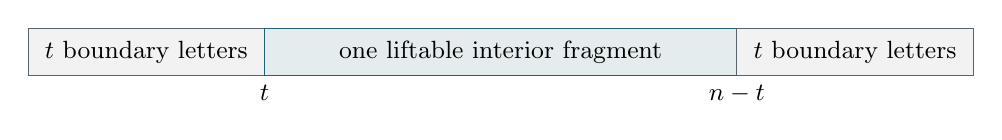
\begin{tikzpicture}[font=\small]
\draw[fill=black!5,draw=Muted] (0,0) rectangle (3,.6);
\draw[fill=Accent!12,draw=Accent] (3,0) rectangle (9,.6);
\draw[fill=black!5,draw=Muted] (9,0) rectangle (12,.6);
\node at (1.5,.3) {$t$ boundary letters};
\node at (6,.3) {one liftable interior fragment};
\node at (10.5,.3) {$t$ boundary letters};
\node[below] at (3,0) {$t$};
\node[below] at (9,0) {$n-t$};
\end{tikzpicture}
\end{center}

\subsection{One obstruction forces linear rank growth}

\begin{theorem}[Periodic pumping of an obstruction]\label{ccc:ps:thm:pumping}
Suppose $v$ is an interior obstruction at a live pair $(r,a)$.
There are fixed words $u,b,z$ with $b\ne\eps$ and $|b|\equiv0\pmod p$
such that, for every $k\ge1$,
\begin{equation}\label{ccc:ps:eq:pump}
 w_k=ub^kz\in\rec(L),\qquad \rank_L(w_k)\ge k+1.
\end{equation}
More strongly, for every sufficiently large $n\equiv r\pmod p$ there is
$w\in\rec(L)_n$ with
\begin{equation}\label{ccc:ps:eq:all-large-lower}
 \rank_L(w)\ge
 \left\lfloor\frac{n-|u|-|z|}{|b|}\right\rfloor+1.
\end{equation}
\end{theorem}
\begin{proof}
Extend $v$ on the right by arbitrary phase-admissible letters until its
length is a positive multiple $h$ of $p$. This is possible because every
coordinate alphabet is nonempty. Call the result $b$. It starts at phase
$a$ and returns to phase $a$, so $b^k$ is phase-admissible for every $k$.
Its first $|v|$ positions in each copy form the same obstruction.

Choose lengths $U,V\ge\max(1,t)$ such that
\[
 U\equiv a\pmod p,\qquad U+V\equiv r\pmod p.
\]
The length $U+V$ is at least $t$ and has live residue, so choose an
accepted word $uz\in L_{U+V}$ with $|u|=U$, $|z|=V$.

We first check all coordinates of $ub^kz$. For a prefix position $i<U$,
the forward length $i$ has not changed. Its suffix length has increased
by $kh$, which is a multiple of $p$, and even the shorter original suffix
length is at least $V\ge t$. Thus \eqref{ccc:ps:eq:fragment-test} for that
single letter has the same truth value as in the accepted word $uz$.
For suffix letters the argument is symmetric: the suffix length is
unchanged and the prefix length increases by $kh$, starting at least
$U\ge t$. All middle letters are in the stable alphabets
$C_{r,a+j}$. Hence every coordinate is allowed, and
$ub^kz\in\rec(L)$.

Now consider any partition of $ub^kz$ into admissible seed fragments.
If one occurrence of $v$ had no cut strictly between its first and last
letters, that whole occurrence would be contained in one fragment.
Restricting the fragment's witnessing seed run to this occurrence would
lift $v$ through its stable viable layers. That contradicts the choice
of $v$. Therefore every occurrence contains an internal partition cut.
The $k$ occurrences are disjoint and each has length at least two, so
their internal boundary sets are disjoint. There are at least $k$ cuts,
hence at least $k+1$ fragments. This proves \eqref{ccc:ps:eq:pump} and, with
Corollary~\ref{ccc:ps:cor:bounded}, completes the necessity in
Theorem~\ref{ccc:ps:thm:criterion}.

For an arbitrary sufficiently large $n\equiv r\pmod p$, write
\[
 n-U-V=kh+d,\qquad 0\le d<h.
\]
Both $n-U-V$ and $h$ are multiples of $p$, so $d$ is a multiple of $p$.
After $b^k$, insert any phase-admissible word $e_d$ of length $d$.
It also returns to phase $a$. The same coordinate argument proves
$ub^ke_dz\in\rec(L)_n$, and the same $k$ disjoint occurrences give
\eqref{ccc:ps:eq:all-large-lower}.
\end{proof}

\begin{corollary}[Residue-wise bounded/linear dichotomy]\label{ccc:ps:cor:residue}
For $n\ge1$, write
\[
 M_L(n)=\max\{\rank_L(w):w\in\rec(L)_n\},
\]
using $M_L(n)=0$ for an empty slice. On each live residue $r$, exactly one
of the following alternatives holds:
\begin{enumerate}
\item $M_L(n)\le2t+1$ for all $n>2t$ in that residue;
\item $M_L(n)=\Theta(n)$ as $n\to\infty$ in that residue.
\end{enumerate}
The second alternative occurs precisely when that residue has an interior
obstruction. It can occur in some residues and not others.
\end{corollary}
\begin{proof}
Apply the central-fragment proof separately to each residue with no
obstruction. Otherwise combine \eqref{ccc:ps:eq:all-large-lower} with
$M_L(n)\le n$. These alternatives cannot overlap.
\end{proof}
\waddsevthree{Part~V sharpens alternative~(2) to $M_L(n)=\sigma_rn+O(1)$
with a rational slope $\sigma_r>0$ (Theorem~\ref{ccc:rs:thm:slope}).}

\begin{corollary}[Asymmetric boundary bound]\label{ccc:ps:cor:asymmetric}
If $P_i$ is $p$-periodic for $i\ge t_P$ and $R_i$ is $p$-periodic for
$i\ge t_R$, then finite stabilization implies
\[
 R(L)\le t_P+t_R+1.
\]
\end{corollary}
\begin{proof}
Use the same stable state sets with separate valid representatives.
The pumping proof works with $U\ge\max(1,t_P)$ and
$V\ge\max(1,t_R)$. If no obstruction exists, keep the central interval
$[t_P,n-t_R)$ as one fragment and use singleton boundary pieces. Shorter
words require at most $t_P+t_R$ singletons.
\end{proof}

\section{Polynomial-space decision and finite obstruction bounds}\label{ccc:ps:sec:space}

\subsection{A finite graph, represented without expansion}

Fix live $r$ and a starting phase $a$. The subset evolution
\eqref{ccc:ps:eq:subset-evolution} is a directed graph on configurations
\[
 (j,Z),\qquad j\in\mathbb Z/p\mathbb Z,\quad Z\subseteq Q.
\]
From $(j,Z)$ a letter $c\in C_{r,j}$ gives
\begin{equation}\label{ccc:ps:eq:graph-edge}
 (j,Z)\longrightarrow
 (j+1,\Delta_c(Z)\cap S_{r,j+1}).
\end{equation}
The initial configuration is $(a,S_{r,a})$, and an obstruction is exactly
a path to an empty-subset configuration.

\begin{lemma}[A short finite obstruction]\label{ccc:ps:lem:short-obstruction}
If an interior obstruction exists at $(r,a)$, one exists of length at most
$p2^s$. It may be padded to a multiple-of-$p$ block of length at most
$p2^s$.
\end{lemma}
\begin{proof}
A shortest path to an empty subset repeats no nonterminal configuration:
a repeated phase and subset could be deleted without changing the
remainder of the path, including its phase-dependent alphabet constraints.
There are at most $p2^s$ configurations. Rounding the resulting positive
length up to a multiple of $p$ does not exceed $p2^s$, since the latter
is itself a multiple of $p$.
\end{proof}

This bound controls an \emph{interior obstruction}, not a rejected word
of the original language and not the length of a full crossover witness.
The exterior words in Theorem~\ref{ccc:ps:thm:pumping} are still needed.

\subsection{The PSPACE upper bound}

\begin{theorem}[Polynomial-space upper bound]\label{ccc:ps:thm:pspace-upper}
For an explicitly given NFA over an explicitly given finite alphabet,
finite constrained self-crossover stabilization, under either clock,
belongs to $\PSPACE$.
\end{theorem}
\begin{proof}
Choose the canonical $t=T_s$ and $p=p_s$. Store $p$ in binary. It has
$O(s\log(s+2))$ bits. For a residue $a$, a suitable representative is
\[
 i_a=t+((a-t)\bmod p).
\]
The sets $P^\infty_a$ and $R^\infty_a$ are computed from $E^{i_a}$ by
Boolean matrix powering. The exponent has polynomially many bits and
the matrices have $s^2$ entries, so this requires polynomial space
(and polynomial time in the bit length of the exponent).

To recognize \emph{nonstabilization}, nondeterministically select residues
$r,a<p$. Check that $r$ is live using \eqref{ccc:ps:eq:live}. Initialize
$j=a$ and $Z=S_{r,a}$. Repeatedly choose a letter $c$, verify
$c\in C_{r,j}$, and update $(j,Z)$ by \eqref{ccc:ps:eq:graph-edge}. Accept if
$Z$ becomes empty. Terminate and reject that branch after $p2^s$ steps.
The counter, phase, residue, subset, transition data, and matrix-powering
workspace all have polynomial size in the input.

Lemma~\ref{ccc:ps:lem:short-obstruction} and Theorem~\ref{ccc:ps:thm:criterion} show
that this nondeterministic machine accepts exactly the nonstabilizing
inputs. Thus nonstabilization is in $\NPSPACE$. Savitch's theorem
\cite{Savitch} gives $\NPSPACE=\PSPACE$, and deterministic polynomial
space is closed under complement. Stabilization is consequently in
$\PSPACE$ too. Corollary~\ref{ccc:ps:cor:bounded} identifies the two clocks.
\end{proof}

For completeness, the resource conversion may also be seen directly.
Reachability in an exponentially large graph with polynomial-bit vertices
can be decided by recursively guessing a midpoint and splitting a path
length in half. A deterministic search enumerates the midpoint encodings.
The recursion depth is logarithmic in the number of configurations, hence
polynomial, and each level stores polynomially many bits. This is the
configuration-graph form of the cited theorem, not an assumption that
nondeterministic time and deterministic time are interchangeable.

\subsection{Quadratic rank and a finite generation cutoff}

\begin{corollary}[Uniform finite horizon]\label{ccc:ps:cor:cutoff}
Let $K_s=\clog{B_s}$. For an $s$-state NFA language, the following are
equivalent:
\[
 \text{finite parallel stabilization},\qquad
 \gen L{K_s}=\rec(L),\qquad
 \gen L{K_s}=\gen L{K_s+1}.
\]
For the frozen-source sequence the corresponding cutoff is $B_s-1$.
\end{corollary}
\begin{proof}
Lemma~\ref{ccc:ps:lem:quadratic-period} and
Theorem~\ref{ccc:ps:thm:criterion} give $R(L)\le B_s$ in the stabilizing case.
Use \eqref{ccc:ps:eq:clocks}. Conversely, any adjacent equality stabilizes the
sequence by monotonicity, independently of the chosen cutoff.
\end{proof}

This is a \emph{uniform cutoff}, not a proposal to construct the enormous
intermediate automata for all generations. The polynomial-space algorithm
tests the periodic interior directly. It is the structural criterion, not
an unrestricted inclusion test on exponentially expanded automata, that
keeps the space bound polynomial.

\begin{corollary}[An explicit full-witness length bound]\label{ccc:ps:cor:witness-length}
If an $s$-state NFA does not stabilize, then, for every integer $q\ge1$,
there is a hull word of rank at least $q+1$ and length at most
\[
 2T_s+2p_s-2+q p_s2^s.
\]
\end{corollary}
\begin{proof}
Use Lemma~\ref{ccc:ps:lem:short-obstruction} for a block of length at most
$p_s2^s$. In the pumping construction, choose $U$ and $V$ in
$[T_s,T_s+p_s-1]$ with their required residues. The word $ub^qz$
has the asserted length and rank.
\end{proof}

In particular, rank just beyond the polynomial bound has a witness of
singly exponential length, with a succinct periodic description. The word
need not itself have a polynomial-length explicit representation.

\section{Binary PSPACE-hardness}\label{ccc:ps:sec:hardness}

\subsection{A factorial-language amplification lemma}

A language is \emph{factorial} if every contiguous factor of every word
in the language also belongs to the language. The language of an NFA in
which every state is both initial and final is factorial: restrict any
accepting path to the interval carrying the desired factor.

\begin{lemma}[Missing factors cannot be repaired in bounded rank]
\label{ccc:ps:lem:factorial}
Let $L\subseteq\{0,1\}^*$ be factorial and contain $0^*\cup1^*$.
Then $\rec(L)=\{0,1\}^*$. Moreover, finite crossover stabilization is
equivalent to $L=\{0,1\}^*$.
\end{lemma}
\begin{proof}
For every $n$ and every coordinate, $0^n$ and $1^n$ supply both possible
letters, and $\eps\in L$. Hence the hull is universal.

If $L$ is not universal, choose $v\notin L$. Because $L$ contains both
unary languages, $v$ has length at least two. No word of $L$ can contain
$v$ as a factor. For the target $v^k$, each of its $k$ disjoint displayed
copies of $v$ must therefore contain an internal partition cut: a seed
fragment containing an entire copy would force $v\in L$. Consequently
$\rank_L(v^k)\ge k+1$. The target is in the universal hull, so rank is
unbounded. Corollary~\ref{ccc:ps:cor:bounded} rules out stabilization. The
universal language is already fixed, proving the converse.
\end{proof}

\subsection{The reduction over two letters}

We use the published result of Kao, Rampersad, and Shallit
\cite[Lemma~6]{KRS}: nonuniversality of binary NFAs with every state both
initial and final is PSPACE-complete. By complement closure, universality
for that class is PSPACE-complete as well. That hardness theorem is an
imported complexity result, not reproved by finite testing here.

\begin{theorem}[Binary hardness with a universal hull]\label{ccc:ps:thm:hardness}
Finite crossover stabilization is PSPACE-hard on binary NFAs. Hardness
persists when all states are initial and final, the language is factorial,
and its coordinate hull is universal. Both iteration clocks have this
property.
\end{theorem}
\begin{proof}
Let $\mathcal A$ be a binary all-initial/all-final NFA recognizing $K$.
Form the disjoint union with one state having only a $0$-loop and one state
having only a $1$-loop. Declare both added states initial and final. The
new automaton recognizes
\begin{equation}\label{ccc:ps:eq:binary-reduction}
 L=K\cup0^*\cup1^*.
\end{equation}
It adds exactly two states. Its language is factorial, and its hull is
universal by Lemma~\ref{ccc:ps:lem:factorial}.

If $K$ is universal, so is $L$. Conversely, if $x\notin K$, then
$x01\notin K$, since otherwise factoriality would put its factor $x$
in $K$. The word $x01$ contains both letters, so it is in neither
$0^*$ nor $1^*$. Thus $L$ is nonuniversal. We have proved
\[
 K=\{0,1\}^*\quad\Longleftrightarrow\quad
 L=\{0,1\}^*\quad\Longleftrightarrow\quad
 L\text{ stabilizes}.
\]
The last equivalence is Lemma~\ref{ccc:ps:lem:factorial}; the reduction is linear
in the automaton size. This proves the result for both clocks.
\end{proof}

\begin{corollary}[Exact complexity and least alphabet]\label{ccc:ps:cor:binary-complete}
Finite constrained self-crossover stabilization is PSPACE-complete for
NFA input over a fixed binary alphabet. Over a unary alphabet every
language, regular or not, is already fixed by constrained self-crossover.
Thus two letters is the least alphabet size permitting the hardness result.
\end{corollary}
\begin{proof}
Combine Theorems~\ref{ccc:ps:thm:pspace-upper} and~\ref{ccc:ps:thm:hardness}.
Over a unary alphabet there is at most one word of each length, so two
same-length parents, if present, are identical. No crossover adds a word.
\end{proof}

The reduction also handles the standard single-initial-state NFA encoding.
Add one fresh initial state, make it accepting because $\eps\in L$, and
on each letter give it the union of the transitions out of the old initial
states. Leave every old transition in place and make only the new state
initial. This $\eps$-free construction adds one state and preserves the
language. The all-initial/all-final promise itself uses the multiple-start
convention, but the ordinary PSPACE-completeness statement does not depend
on that convention.

\subsection{A second reduction connecting to the repository amplifier}

The preceding proof is the sharper alphabet result. The following
four-letter version explains directly how the old report's delimiter
amplification also yields a hardness proof from ordinary binary NFA
universality. Its block mechanism is credited to that earlier line of
argument; it is not a second claimed discovery of the amplifier.
\wsix\ The amplifier is Part~I's Theorem~\ref{ccc:thm:amplification}, with
the context-free languages $G_K$ and $B_K$ of
\eqref{ccc:eq:guardlanguage}--\eqref{ccc:eq:blocklanguage}; the regular
languages $\widehat G(K)$, $\widehat B(K)$ below (the manuscript's $G(K)$,
$B(K)$) are different: $\widehat G(K)$ adds to $K$ every word containing~$@$,
with no $00$ guard, and $\widehat B(K)$ leaves its first and last blocks
unrestricted.

Let $K\subseteq\{0,1\}^*$ be given by an NFA, let
$\Gamma=\{0,1,@\}$, and put
\[
 \widehat G(K)=K\cup\Gamma^*@\Gamma^*,\qquad
 \widehat B(K)=\Gamma^*\ \cup\ \Gamma^*\#(\widehat G(K)\#)^*\Gamma^*.
\]
An internal complete $\#$-delimited block must lie in $\widehat G(K)$; the first
and last incomplete blocks are unrestricted. Standard union, concatenation,
and star constructions give an NFA of size linear in the input, and
$\eps$-elimination preserves the state set.

\begin{proposition}[Exact delimiter ranks]\label{ccc:ps:prop:delimiter}
The hull of $\widehat B(K)$ is $\{0,1,@,\#\}^*$. If $K$ is universal, so is
$\widehat B(K)$. If $x\notin K$, then for every $q\ge1$,
\[
 \rank_{\widehat B(K)}\bigl(\#(x\#)^q\bigr)=q+1.
\]
\end{proposition}
\begin{proof}
A word with at most one delimiter belongs to $\widehat B(K)$. For any prescribed
letter at any prescribed position, fill every other position with $@$
to obtain such a seed. This proves the hull assertion, including the
empty word.

If $K$ is universal, $\widehat G(K)=\Gamma^*$ and the displayed expression for
$\widehat B(K)$ permits every word. If $x\notin K$, each displayed $\#x\#$ in
$\#(x\#)^q$ is forbidden inside a seed. Consecutive occurrences may
share a delimiter letter, but their \emph{internal boundary slots} are
disjoint. Hence every fragment partition needs at least $q$ cuts.
For the opposite bound, partition as $q$ copies of $\#x$ and one final
$\#$. Each piece contains at most one delimiter and extends to a
length-matched seed by filling outside positions with $@$. These are
$q+1$ admissible fragments. If $x=\eps$, the same argument partitions
$\#^{q+1}$ into single letters and remains valid.
\end{proof}

This establishes the four-letter reduction without the all-initial/all-final
hardness theorem. It is included for comparison and proof portability; the
binary theorem above remains the stronger final result.

\section{Deterministic automata and safe cores}\label{ccc:ps:sec:dfa}

Assume now that each $\Delta_c(q)$ has at most one state. The original
DFA may be complete, but after restriction to viable phase sets some
transitions become undefined. Fix a live residue $r$ and regard
\[
 (a,q),\qquad q\in S_{r,a},
\]
as vertices of a partial deterministic phase graph. Its allowed input
letters at phase $a$ are $C_{r,a}$.

\begin{definition}[Safe core]\label{ccc:ps:def:safe-core}
A family $(U_a)_{a\bmod p}$ with $U_a\subseteq S_{r,a}$ is safe if
\[
 q\in U_a,
 \ c\in C_{r,a}
 \quad\Longrightarrow\quad
 \delta(q,c)\text{ is defined and belongs to }U_{a+1}.
\]
The safe core $(\Core_{r,a})$ is the greatest such family.
\end{definition}

It is obtained by starting with all viable vertices and repeatedly deleting
any vertex with an allowed letter leading outside the surviving set.
The process terminates after at most $ps$ vertex deletions. An efficient
implementation stores reverse edges and a queue of newly unsafe vertices.

\begin{theorem}[Safe-core characterization]\label{ccc:ps:thm:core}
For a deterministic automaton and a fixed live residue $r$, all
phase-admissible words are liftable at every starting phase if and only if
the safe core is nonempty. A nonempty safe core meets every phase.
\end{theorem}
\begin{proof}
If a safe vertex exists, any allowed letter takes it to a safe vertex in
the next phase. Following one allowed letter at a time, possible because
all $C_{r,a}$ are nonempty, shows that safe vertices exist in every phase.
Starting with any safe vertex at a desired phase then reads every
phase-admissible word without leaving the viable graph. This proves
sufficiency.

Suppose the safe core is empty. A vertex is safe exactly when no
phase-admissible continuation can cause its deterministic run to leave
the viable graph. Equivalently, every vertex now has some killing
continuation. One can see this directly from deletion times: a vertex
removed first has an immediately invalid allowed transition; a later
removed vertex has a transition to an earlier removed vertex.

Start with all viable states at some phase. Select one survivor and append
a killing word for that survivor. The statewise determinism implies that
every current state has at most one resulting image. Since the selected
state has no image, the number of surviving images drops by at least one.
Repeat with a surviving state at the new phase. After at most $s$ rounds
there are no survivors. The concatenated word is phase-admissible but
not liftable. Thus universality fails.
\end{proof}

\begin{corollary}[A shorter deterministic obstruction]\label{ccc:ps:cor:dfa-obstruction}
If a live residue of a deterministic $s$-state automaton has an interior
obstruction, it has one of length at most $ps^2$.
\end{corollary}
\begin{proof}
When the safe core is empty, a shortest route from any given vertex to
an invalid allowed transition traverses no vertex twice before failure.
It has length at most the number of phase vertices, at most $ps$.
Use such a route in each of at most $s$ killing rounds in the proof of
Theorem~\ref{ccc:ps:thm:core}.
\end{proof}

For a fixed residue with its phase sets explicitly listed, the safe core
can be computed in $O(ps|\Sigma|)$ time by backward deletion. Treating all
$p$ residues separately gives $O(p^2s|\Sigma|)$ core work, in addition to
constructing the phase sets. These are bounds in the \emph{expanded
periodic presentation}. Since $p$ can be exponentially large relative to
the original state count, this is not a polynomial-time algorithm for
arbitrary DFA input. The PSPACE upper bound still follows from
Theorem~\ref{ccc:ps:thm:pspace-upper}; no matching DFA lower bound is claimed.

\begin{example}[Why the deterministic argument cannot be used on NFAs]
\label{ccc:ps:ex:nondeterministic}
Take two states $x,y$, both initial and final, with transitions
\[
 \Delta_0(x)=\{x,y\},\quad \Delta_1(x)=\varnothing,\qquad
 \Delta_0(y)=\varnothing,\quad \Delta_1(y)=\{x,y\}.
\]
The language is all binary words: after any letter the full two-state
subset is available again. Yet neither individual state supports both
possible first letters. A vertexwise safety deletion removes both states,
even though the subset evolution never empties. The deterministic
cardinality-drop argument fails because a single NFA state can branch
into several surviving states. This is a concrete reason to retain subset
universality in the NFA algorithm.
\end{example}

\section{Quantitative consequences and worked examples}\label{ccc:ps:sec:examples}

\subsection{The generation bound has the right logarithmic order}

\begin{theorem}[Logarithmic generation lower bound]\label{ccc:ps:thm:lower-family}
For each $m\ge1$, let
\[
 L_m=\{0^{i-1}1\,0^{m-i}:1\le i\le m\}.
\]
This language has a complete DFA with at most $2m+3$ states, stabilizes
finitely, and satisfies $R(L_m)=m$. Its least parallel stabilization index
is $\clog m$, and its least frozen-source index is $m-1$.
\end{theorem}
\begin{proof}
A DFA stores the current length $0,\ldots,m$, whether a $1$ has already
occurred, and one rejecting sink. Moving past length $m$ or seeing a
second $1$ enters the sink. This uses $2(m+1)+1$ states; unreachable
states may be removed but are irrelevant to the bound.

All nonempty hull words have length $m$, so rank is at most $m$.
Every coordinate of $1^m$ is supplied by one of the seed words. No
admissible fragment of $1^m$ can have length at least two, because a
seed has only one $1$. Hence $\rank_{L_m}(1^m)=m$. The case $m=1$
is included, with rank one. Apply Corollary~\ref{ccc:ps:cor:bounded}.
\end{proof}

Thus the largest possible finite parallel stabilization index for
$s$-state automata has order $\Theta(\log s)$, even over two letters.
This does \emph{not} prove that the quadratic rank bound is optimal.
The presently proved lower and upper orders for maximal finite rank are
linear and quadratic, respectively.
\waddsevone{Part~IV raises the lower order to quadratic for NFAs:
Theorem~\ref{ccc:qr:thm:main} gives an $s$-state NFA with finite maximal
rank $(s-3)^2$, so the quadratic rank bound has the optimal order (its
constant is open), and the parallel index of order $\Theta(\log s)$ is
$2\log_2s+O(1)$ (Section~\ref{ccc:qr:sec:upper}). The family $L_m$ above has
a complete DFA; for DFAs the lower order in this report stays linear
(Question~\ref{ccc:qr:q:dfa}).}

\subsection{A regular language with a repairable boundary}

\begin{example}[One generation without universality]\label{ccc:ps:ex:boundary}
Over $\Sigma=\{0,1\}$, let
\[
 L=\{\eps\}\cup0\Sigma^*\cup\Sigma^*0.
\]
Then $\rec(L)_1=\{0\}$ and $\rec(L)_n=\Sigma^n$ for $n\ge2$.
For any $w\in\Sigma^n$ with $n\ge2$, choose an interior cut.
The prefix is supplied by a seed ending in $0$ and the suffix by a seed
starting in $0$. Hence rank is at most two and $T(L)=\rec(L)$.
The word $11$ is not a seed and has rank exactly two, so the least
parallel and frozen-source indices both equal one.

This example separates finite stabilization from universality for general
regular languages. The hardness equivalence with universality applies to
the special factorial class, not to all NFAs.
\end{example}

\subsection{Bounded and linear residues can coexist}

\begin{example}[Even lengths are fixed; odd lengths have linear rank]
\label{ccc:ps:ex:parity}
Let
\[
 L=\{w\in\{0,1\}^*:|w|\text{ is even}\}\cup0^*\cup1^*.
\]
Its hull is universal. At even lengths every word is a seed, so the
maximum rank is one. At odd lengths the seeds are exactly $0^n,1^n$;
an admissible nonempty fragment must be constant. Therefore the rank of
an odd-length word is its number of maximal constant runs, and
\[
 M_L(n)=\begin{cases}1,&n\text{ even},\\n,&n\text{ odd}.
 \end{cases}
\]
Here $M_L(0)$ may also be taken as one. A four-state NFA recognizes the
language by taking a disjoint union of a parity automaton and two unary
loops. The periodic criterion sees a universal interior at the even total
residue and an obstruction such as $01$ at the odd residue.
\end{example}

The example shows why a statement of linear growth at \emph{all} large
lengths would be false. It also explains why the total-length residue $r$
and the boundary phase $a$ are separate parameters in the construction.

\subsection{The strongest possible generation growth in a bad residue}

On a live residue with an obstruction, let
\[
 D_L(n)=\max_{w\in\rec(L)_n}\min\{k:w\in\gen Lk\}.
\]
By \eqref{ccc:ps:eq:clocks} and Corollary~\ref{ccc:ps:cor:residue},
\begin{equation}\label{ccc:ps:eq:depth-asymptotic}
 D_L(n)=\log_2 n+O(1)
 \quad(n\to\infty\text{ in that residue}).
\end{equation}
The maximum frozen-source depth is $M_L(n)-1=\Theta(n)$. The constants
can be read from the pumped block length and boundary lengths. In a good
residue the two depths remain bounded. Thus the rank dichotomy yields a
complete bounded-versus-maximal-order dichotomy for the two natural
iteration clocks, residue by residue.

\section{Executable audits and their limits}\label{ccc:ps:sec:audits}

The package contains a standard-library Python implementation in
\nolinkurl{code/verify.py}. It is an exact finite reference checker, not
an optimized prover and not a formalization. Its NFA transitions and
subsets are represented by integer bit masks. The recorded run used
Python 3.13.5 and returned \texttt{PASS}; details and limitations are
stored in \nolinkurl{data/verification.json} and the console transcript
\nolinkurl{data/verification.txt}.

\wsix\ \emph{Shipped names.} In this report the delivered files are shipped,
byte-identical, as follows; the manuscript and its PDF are printed or
replaced by this report, and the delivery README by the report's README. The
unprefixed \nolinkurl{data/verification.json} of this report is Part~I's
receipt (Section~\ref{ccc:sec:verification}).
\begin{center}\footnotesize
\begin{tabular}{@{}L{.58\textwidth}L{.36\textwidth}@{}}
\toprule
\textbf{Shipped path} & \textbf{Delivered as}\\
\midrule
\nolinkurl{code/02-pspace-stabilization-verify.py} & \texttt{code/verify.py}\\
\nolinkurl{code/02-pspace-stabilization-example.py} & \texttt{code/example.py}\\
\nolinkurl{code/02-pspace-stabilization-build.sh} & \texttt{build.sh}\\
\nolinkurl{data/02-pspace-stabilization-verification.json} & \texttt{data/verification.json}\\
\nolinkurl{data/02-pspace-stabilization-verification.txt} & \texttt{data/verification.txt}\\
\nolinkurl{data/02-pspace-stabilization-build-receipt.json} & \texttt{data/build-receipt.json}\\
\nolinkurl{02-pspace-stabilization-proof-audit.md} & \texttt{notes/proof-audit.md}\\
\nolinkurl{02-pspace-stabilization-source-ledger.md} & \texttt{notes/source-ledger.md}\\
\bottomrule
\end{tabular}
\end{center}

\subsection{Two independent rank calculations}

The path-based algorithm implements \eqref{ccc:ps:eq:rank-dp}. The independent
algorithm enumerates all accepted seed words at a given length, collects
their actual aligned substrings, and runs a partition dynamic program on
those substring sets. In particular, it does not use $P_i$, $R_j$, or
viable layers to decide interval admissibility. All tested finite ranks,
including infinity and the empty-word case, agreed.

The literal crossover check enumerates all parent pairs and cuts. It then
compares its actual generated sets with the rank thresholds $2^k$.
These checks are logically separate from the periodic criterion.

\subsection{Recorded coverage}

\begin{center}\small
\begin{tabular}{@{}L{.67\textwidth}r@{}}
\toprule
Exact audit & Recorded count\\
\midrule
All labelled two-state binary NFAs, all initial/final subsets & 4,096\\
Independent rank comparisons, all binary words of lengths $0$--$5$ & 258,048\\
Stable-rank bound checks within those comparisons & 69,488\\
Complete three-state binary DFAs, fixed initial state & 5,832\\
Safe-core versus subset-criterion comparisons on those DFAs & 5,832\\
Stable three-state DFA rank checks at length $6$ & 369,152\\
Additional partial-deterministic core comparisons & 1,296\\
Pumped-witness checks across the stated families & 1,641\\
Binary all-initial/all-final hardness-transform cases & 256\\
All binary finite seed sets on slices of lengths $0$--$3$ & 278\\
Literal parallel-generation comparisons on those seeds & 1,112\\
One-$1$ lower-family cases, $1\le m\le24$ & 24\\
Unary graph/subset cases on $1$--$3$ vertices & 4,164\\
Unary periodicity equalities within those cases & 4,382\\
Exact delimiter ranks, including the omitted empty word & 504\\
Delimiter coordinate-supply witnesses & 9,072\\
Parity-example rank checks, lengths $1$--$10$ & 2,046\\
Boundary-repair example rank checks, lengths $0$--$7$ & 255\\
\bottomrule
\end{tabular}
\end{center}

The two-state NFA family has 3,720 stabilizing and 376 nonstabilizing
members according to the implemented exact periodic criterion. The
three-state complete DFA family has 5,768 stabilizing and 64
nonstabilizing members. These are labelled-automaton counts, not counts
of distinct languages or isomorphism classes.

An additional 200 seeded random NFAs with three through six states were
tested, with 4,000 sampled rank queries. The seed is \texttt{20260930}.
Those samples are explicitly not exhaustive. The worked examples are also
checked directly: the delimiter family uses every omitted binary word of
length at most five and one through eight repeated blocks; the parity
example uses every binary word of lengths one through ten; and the
boundary-repair example uses every binary word of length at most seven. The unary audit enumerates
every directed graph on one through three labelled vertices and every
chosen initial subset, taking the same subset as final; it tests both
forward and backward sequences through their exact eventual cycles.

The categories overlap: for example, some of the rank-bound checks are
also independent rank comparisons. Their counts must not be added and
reported as a number of statistically independent experiments.

\subsection{What the program actually certifies}

The periodic solver explicitly enumerates the least eventual cycle of
$(P_i,R_i)$ and then searches phase/subset graphs by breadth first search.
On the tested small automata this is convenient, but it stores the
expanded graph. It is \emph{not} an implementation with the polynomial-space
resource guarantee of Section~\ref{ccc:ps:sec:space}. The latter is an
on-the-fly theoretical algorithm with binary counters and matrix powers.

For each detected small obstruction, the program constructs the exterior
accepted word and the padded repeated block from the proof, then verifies
finite ranks of the resulting full words. On stabilizing cases it checks
the stronger observed-transient bound $2t+1$, where $t$ is obtained from
the least pair cycle, rather than only the much looser universal $B_s$.

No finite test proves that every rank above every state count is bounded,
or that every obstruction pumps. Those are theorems proved in
Sections~\ref{ccc:ps:sec:dichotomy}--\ref{ccc:ps:sec:space}. No solver is used to infer
PSPACE-hardness, no verification output is represented as a Lean kernel
certificate, and no literature theorem is declared proved because small
instances pass.

\subsection{Reproduction}

From the package root, run
\begin{lstlisting}
python3 code/verify.py --output data/local-verification.json
latexmk -pdf -interaction=nonstopmode -halt-on-error article.tex
\end{lstlisting}
The explicit output option preserves the delivered receipt. The default
output path is \nolinkurl{data/verification.json}; running without the
option replaces that file in the local copy. There are no network calls,
third-party Python dependencies, or external theorem provers in the
checker. The included build script performs only the local LaTeX build.

\wsix\ \emph{In this report, do not run the shipped files in place.} The
verifier's default output path is \nolinkurl{../data/verification.json}
relative to its own directory, which here is Part~I's receipt; the example
program imports the verifier under its delivered module name
\texttt{verify}, which the prefixed file does not have; and the build script
runs \texttt{latexmk} on an \texttt{article.tex} in its own directory,
\texttt{code/}, where there is none. Copy the two programs into a scratch
directory under their delivered names \texttt{code/verify.py} and
\texttt{code/example.py}, and run them there, with an explicit
\texttt{-{}-output}; the report's README gives the commands and the result of
such a rerun. The article is rebuilt from the report directory as in
Section~\ref{ccc:sec:verification}. The delivered example program's comment
calls the parity language ``article Example~9.3''; in this report it is
Example~\ref{ccc:ps:ex:parity}.

\section{Further research questions}\label{ccc:ps:sec:questions}

The questions below are specific continuation targets. They are not all
asserted to be new or globally open. The first is the unsolved portion of
the inspected report's regular-input complexity question; the others are
natural sharpenings exposed by the present proofs.
\wsix\ The inspected report's question is Part~I's
Question~\ref{ccc:q:regular}. Question~\ref{ccc:ps:q:cfg} below is Part~I's
Question~\ref{ccc:q:arithmetical} and is printed as a pointer;
Question~\ref{ccc:ps:q:restricted} overlaps Part~I's
Question~\ref{ccc:q:restricted}, asking it for the dichotomy proved here.

\begin{question}[Exact complexity for DFA input]\label{ccc:ps:q:dfa}
What is the exact complexity of deciding finite stabilization for complete
DFAs over a fixed binary alphabet?
\end{question}
The present PSPACE upper bound is stronger than the earlier EXPSPACE
bound, but the NFA hardness proof does not transfer to a DFA without an
exponential determinization. The safe-core characterization removes
subset branching once the phases are explicit. The remaining issue is
whether the exponentially long unary phase structure can be manipulated
more economically, or can encode a matching hard problem. An algorithm
polynomial in $p$ does not answer this question.

\begin{question}[The optimal finite rank bound]\label{ccc:ps:q:rank}
Let $F(s)$ be the largest finite $R(L)$ among binary languages recognized
by NFAs with at most $s$ states. Is $F(s)$ linear, quadratic, or of an
intermediate order?
\end{question}
There are only finitely many labelled NFAs of a fixed state bound, so
this maximum is well defined. For $s\ge5$, the results here give
\[
 \left\lfloor\frac{s-3}{2}\right\rfloor
 \le F(s)\le(2s+5)^2.
\]
A quadratic lower bound would have to exploit long unary transients while
making many boundary positions require genuinely separate aligned
fragments. A long transient alone is not such a proof. Conversely, a
linear upper bound would need a way to compress boundary fragments that
is absent from the singleton argument.
\waddsevone{Answered as to order, for NFAs, in Part~IV:
$(s-3)^2\le F(s)\le(2s+5)^2$ for $s\ge4$, so $F(s)=\Theta(s^2)$
(Theorem~\ref{ccc:qr:thm:main}). The construction takes the route sketched
above: a long unary length transient (a two-cycle length gate) together
with two monochromatic components, which make every change of letter at a
missing length a boundary between separate fragments. The upper bound is the
one above. The leading constant and the exact $F(s)$ stay open
(Question~\ref{ccc:qr:q:constant}), and so does the order for DFAs
(Question~\ref{ccc:qr:q:dfa}).}
\waddsevthree{Part~V lowers the upper bound to $2(s-1)^2+3$
(Corollary~\ref{ccc:rs:cor:upper}), so that $(s-3)^2\le F(s)\le2(s-1)^2+3$
and the leading constant lies in $[1,2]$.}

\begin{question}[Exact residue-wise rank slope]\label{ccc:ps:q:slope}
On a bad residue, does $M_L(n)/n$ always have a limit, perhaps after
refining the period? Must a resulting slope be rational, and can it be
computed effectively?
\end{question}
The pumping theorem gives positive lower and upper linear bounds, not
a limit or a formula. The quantity is a maximum over target words of a
minimum partition cost. Replacing it by a shortest-path mean without
justifying this order of quantifiers would be invalid. The periodic
systems provide finite objects on which this problem can be studied.
\waddsevthree{Answered in all three parts by Part~V
(Theorem~\ref{ccc:rs:thm:slope}): on every live residue $r$ of any valid
period, $M_L(n)=\sigma_rn+O(1)$, where $\sigma_r$ is rational with denominator
at most $p(2^s-1)$, is computed as the largest reachable cycle mean of a
finite subset-reset graph, and is positive exactly when the residue has an
interior obstruction; no refinement of the period is needed. The order of
quantifiers is handled as asked above: longest-prefix greedy factorization is
optimal (Lemma~\ref{ccc:rs:lem:greedy}), so the minimum partition cost is
computed by a deterministic parser before any maximization.}

\begin{question}[Optimal obstruction lengths]\label{ccc:ps:q:length}
How sharp are the interior bounds $p2^s$ for NFAs and $ps^2$ for DFAs?
Can the multiplicative $p$ be replaced by a smaller invariant of the
unary reachability graph?
\end{question}
The NFA bound is a configuration-count bound; the DFA bound concatenates
at most $s$ single-state killing words. Neither construction is claimed
optimal. The definition of an interior obstruction must be retained:
shortest nonmembers of $L$ can instead reflect only a repairable boundary.

\begin{question}[Compressed periods and effective certificates]\label{ccc:ps:q:period}
Can the live residues and their safe or obstructed status be represented
by polynomial-size arithmetic data, rather than by all residues modulo
an explicit least common multiple?
\end{question}
The common period used here is convenient but often highly redundant.
Strongly connected component periods and arithmetic-progressions
representations are candidate data structures. A positive certificate
would need to establish universality in every live phase system, not
merely exhibit a few successful runs. A negative certificate can already
be represented by one forbidden interior word and periodic exterior
padding, but that word may itself be exponentially long.

\begin{question}[Context-free finite stabilization]\label{ccc:ps:q:cfg}
\wsix\ This is Part~I's Question~\ref{ccc:q:arithmetical}, printed there:
what is the exact arithmetical complexity of finite stabilization for
context-free grammar input under the same aligned operation? The
manuscript's comment follows.
\end{question}
The inspected report proves undecidability and gives an upper placement
in $\Sigma^0_2$ (Theorem~\ref{ccc:thm:eventual} and
Proposition~\ref{ccc:prop:arithmetical}), but does not claim completeness at that level. Nothing
in the regular-input analysis resolves this question: unary periodicity
of the two exact-length state processes uses finiteness of the automaton
state set. A reduction showing unbounded rank from the failure of a
$\Sigma^0_2$ property would require a different argument.

\begin{question}[Restricted cuts and other recombination rules]
\label{ccc:ps:q:restricted}
Which parts of the dichotomy survive when only a regular set of cut
positions is permitted, or when a single operation exchanges several
alternating intervals between two parents?
\end{question}
For unrestricted aligned one-point self-crossover, every singleton is
available in the eventual hull. Restricted cuts may destroy that product
structure. In a multi-cut operation, several pieces still come from only
two parents; they are not automatically independent fragments. Thus one
cannot simply replace the factor two in the rank law by the number of
cuts plus one without proving an appropriate realization theorem.

\begin{question}[Proof-assistant implementation]\label{ccc:ps:q:formal}
Can the periodic-interior equivalence, quantitative cutoff, and binary
hardness reduction be formalized with an auditable separation between
combinatorial proofs and imported complexity theorems?
\end{question}
The development proposed in the next section gives small independent
milestones. Formalizing the full PSPACE lower bound includes the published
all-initial/all-final universality reduction, not merely the two-state
union construction used here.
\waddsevone{Part~IV's Question~\ref{ccc:qr:q:formal} asks the same for its
lower-bound construction.}

\section{A formalization and implementation roadmap}\label{ccc:ps:sec:formal}

No Lean or Rocq files are claimed as verified in this delivery. A practical
formal development can nevertheless be organized without importing the
entire earlier report as an unexamined axiom.

\paragraph{Finite words and partitions.}
Define an aligned interval by two bounded natural numbers and a proof of
their strict order. Define fragment admissibility by a length-matched
witness word. The two rank thresholds can first be stated as existence
of a partition with at most $d$ pieces, avoiding extended-natural minima
until the basic equivalences have been proved. The empty-word convention
should be isolated at the start.

\paragraph{Runs and exact-length reachability.}
Represent an NFA by finite relations on a finite state type. Prove
Lemma~\ref{ccc:ps:lem:fragment} by concatenating and restricting finite runs.
This is the bridge at which absolute coordinates and total lengths must
be retained. The periodic theorem can initially take $t,p$ and the
periodicity equations as explicit hypotheses.

\paragraph{The structural core.}
Prove the central-fragment sufficiency result first. Then prove the
pumping lemma in three separate pieces: phase-aligned block extension,
preservation of each exterior coordinate under a multiple-of-period
length change, and the injection from obstruction copies to partition
cuts. The last piece uses the strict internal boundary sets; it does not
need a vague claim that copies are ``independent''.

\paragraph{Quantitative periodicity.}
The elementary $4^s$ eventual-cycle argument is a short finite-state
lemma and can yield a fully formal qualitative result early. The
quadratic bound should be added only after a verified unary
arithmetic-progression theorem is available, or else recorded as an
explicit conditional corollary. The two added normalization states and
the length shift by two must not disappear from the statement.

\paragraph{Decision complexity.}
A reference explicit algorithm is much easier to validate than its space
bound. Separate functional correctness of the phase/subset search from
the representation-size proof for binary counters, Boolean matrix
powering, and nondeterministic configuration graphs. Likewise, prove the
binary language equivalence in \eqref{ccc:ps:eq:binary-reduction} independently
of importing PSPACE-completeness of the source problem.

\paragraph{Deterministic safety.}
The greatest safe family is a finite greatest fixed point. Its elementary
delete-to-failure proof should be particularly tractable. The proof that
killing one deterministic start decreases the surviving-subset
cardinality should be a named lemma, making the exact point where
nondeterminism breaks the argument explicit.

These milestones produce useful formal theorems before a full complexity
library is available. They also keep the distinction between an existing
repository formalization, an ordinary mathematical proof, and a future
formalization plan visible.

\section{Conclusion}\label{ccc:ps:sec:conclusion}

The special two-sided structure identified in the repository question
really does improve on generic limitedness. Exact-length reachability
becomes periodic from both ends. In a good interior, all allowed target
letters can be joined by one seed run, leaving only a bounded exterior
cost. In a bad interior, one finite failure repeats and forces a fresh
partition cut each time. This yields both the bounded/linear dichotomy
and a finite search problem on phase/subset configurations.

As a consequence, finite stabilization for NFA input is PSPACE-complete
over the smallest nontrivial alphabet, while every stabilizing $s$-state
instance has rank at most $(2s+5)^2$. The logarithmic order of the parallel
generation bound is sharp. The exact DFA complexity, optimal rank order,
and precise slopes of bad residues remain substantive next problems,
rather than being hidden inside an unspecified generic limitedness bound.
\waddsevone{The optimal rank order is now known for NFAs: it is quadratic
(Part~IV, Theorem~\ref{ccc:qr:thm:main}); its constant and the DFA case
remain.}
\waddsevthree{The slopes of bad residues are now determined: they are
rational and effectively computable (Part~V,
Theorem~\ref{ccc:rs:thm:slope}), and the constant of the rank order is at
most two (Corollary~\ref{ccc:rs:cor:upper}).}

\section{Proof and edge-case audit}\label{ccc:ps:app:audit}

\wsix\ This section and the next were the manuscript's Appendices~A and~B.

\begin{longtable}{@{}L{.28\textwidth}L{.66\textwidth}@{}}
\toprule
Potential failure & How the proof handles it\\
\midrule
\endhead
Empty language or empty slice & There is no live contribution; hull slices remain empty. $R(L)$ includes $1$ only to normalize the empty-language stabilization index.\\[4pt]
The empty word & Its rank is $1$ exactly when it is a seed. The length-zero hull is explicitly $L_0$, not an unconditional empty product.\\[4pt]
Transient $t=0$ & The central-fragment argument then gives rank $1$ in the stabilizing case. Pumping uses positive exterior lengths to avoid vacuous baselines.\\[4pt]
An obstruction of length one & Impossible by the definition of $C_{r,a}$; every permitted letter has a viable transition. Thus every obstruction has an internal cut slot.\\[4pt]
A forbidden word only at a particular phase & The padded block has length divisible by $p$, so every copy starts at the same phase.\\[4pt]
The total-length residue changes & It does not: all inserted block and remainder lengths are multiples of $p$.\\[4pt]
Exterior coordinates cease to be available & The unchanged side of the single-letter path test is exact; the changed side lies beyond its transient and changes by a multiple of $p$.\\[4pt]
A fragment's parent run is not globally fixed & Each admissible fragment has its own seed witness. Restricting that witness is sufficient to contradict an interior obstruction.\\[4pt]
Linear growth only on a sparse subsequence & The remainder-padding step supplies every sufficiently large length of the chosen residue, not merely lengths of the form $U+kh+V$.\\[4pt]
Confusing a huge period with a huge rank bound & The period is used to build and recognize the interior. Rank cost comes from the two transients, which are quadratic independently of the period.\\[4pt]
Replacing NFA universality by statewise safety & The two-state example in Section~\ref{ccc:ps:sec:dfa} disproves that replacement. Safety is used only for deterministic transitions.\\[4pt]
Binary hardness filled by unary loops & A missing word $x$ in a factorial language forces the missing mixed word $x01$, so adding $0^*\cup1^*$ cannot create false universal cases.\\[4pt]
Sharing a delimiter in the second reduction & The forbidden occurrences share a letter, not an internal boundary slot. Their required cuts remain distinct, including $x=\eps$.\\[4pt]
Claiming a polynomial-time DFA algorithm & The safe-core time is polynomial only in the expanded period. The article does not identify it with polynomial time in the original automaton.\\[4pt]
Finite checks presented as a proof & They are bounded audits. Universal claims rest on the written arguments and the explicitly cited imported theorems.\\
\bottomrule
\end{longtable}

\section{Source ledger and novelty boundary}\label{ccc:ps:app:sources}

\paragraph{Repository source.}
The pinned source is the crossover report's \nolinkurl{article.tex} and
\nolinkurl{README.md} at the revision displayed in
Section~\ref{ccc:ps:sec:intro}. The EXPSPACE upper bound is its corollary headed
\emph{Decidable regular-input stabilization}; the continuation target is
its Section~11 question headed \emph{Sharp regular-input complexity}.
The rank formulas and frozen-source calculus are credited background.
The report itself states that it is unrefereed and not formalized.
\wsix\ These are Part~I's Corollary~\ref{ccc:cor:regularstability} and
Question~\ref{ccc:q:regular}; the source ledger is shipped as
\nolinkurl{02-pspace-stabilization-source-ledger.md}.

\paragraph{Primary external inputs.}
The aligned operation was checked against Hughes's version~1 preprint.
The corrected unary constants were checked in To's Section~3, including
the page images of the correction. The binary all-initial/all-final
universality hardness was checked against Lemma~6 of the version~2
Kao--Rampersad--Shallit preprint. Savitch's space simulation is the
standard complexity conversion used for the upper bound; the argument's
configuration-graph application is explained in the text.

\paragraph{What is imported, and what is proved here.}
The unary arithmetic-progression theorem and the PSPACE-hardness of the
source universality problem are imported published results. The
periodic-interior criterion, obstruction pumping theorem, rank and depth
consequences, crossover complexity reduction, and deterministic safe-core
application are proved in this article. The earlier rank calculus is
reproved for completeness, not claimed as a new contribution.

\paragraph{Search boundary.}
Searches on 30 September 2026 included combinations of constrained
crossover, finite stabilization, regular languages, recombination,
PSPACE, unary arithmetic progressions, and all-initial/all-final NFA
universality. Broad recombination searches were noisy and did not amount
to an exhaustive literature classification. The defensible novelty claim
is a proved extension of the inspected repository, not an unconditional
assertion of worldwide priority or a claim of peer-reviewed acceptance.

\paragraph{No hidden formal status.}
No assertion in this article was checked by Lean or Rocq. The Python
program and its receipts are included so that the finite audits can be
reproduced, but the ordinary proofs remain independently reviewable.
No repository file was modified as part of this delivery.

\wsix\ The last sentence describes the delivery; the write phase added this
Part and dated notes in Part~I. Placement beside ProveIt's Lean and Rocq
developments confers no formal status on Part~II, and none of its statements
is formalized. No ProveIt Lean or Rocq file defines finite automata,
crossover, aligned rank, unary arithmetic-progression normal forms or space
complexity classes, so To's theorem, Kao--Rampersad--Shallit's Lemma~6 and
Savitch's theorem enter only as cited mathematics.

%% =====================================================================
%% [write] Batch-66 addition 03: manuscript 03 of batch 66, "Decidable
%% Regularity and Exact Stabilization of Crossover Closures". Every label
%% of this Part carries the prefix ccc:cl: (closure classification).
%% =====================================================================
\clearpage
\phantomsection\part*{Part III.\quad Decidable regularity and exact stabilization of crossover closures}
\addcontentsline{toc}{part}{Part III.\texorpdfstring{\quad}{ } Decidable regularity and exact stabilization of crossover closures}

\noindent\emph{\wsix\ Part~III was added on 30 September 2026 in batch~66,
together with Part~II, from a second manuscript written against Part~I as
printed above (it did not know Part~II). For context-free seeds it decides
regularity, inclusion and equality of the full crossover closures; for
semilinear one-marker seeds it computes every generation, decides finite
stabilization, and classifies the stabilizing ones into regular, linear
non-regular and non-context-free closures; and it shows exact stabilization
depth to be a clique number, coNP-complete to threshold for succinct ray
input. It partly answers Part~I's Question~\ref{ccc:q:grammar}. It shares
with Part~II only a reproof of Part~I's coordinate hull, printed here as a
third route (Lemma~\ref{ccc:cl:lem:hull}). Section~\ref{ccc:cl:sec:provenance}
records the provenance and fixes the notation of the addition.}

\section{\texorpdfstring{\wsix\ }{}Provenance and notation of Part~III}
\label{ccc:cl:sec:provenance}

\subsection{One manuscript, one addition}\label{ccc:cl:sec:source}

Part~III is batch-66 manuscript~03, \emph{Decidable Regularity and Exact
Stabilization of Crossover Closures: arithmetic invariants, sparse-marker
trichotomies, and immediate loss of context-freeness}, dated 30 September
2026 (23 US-letter pages as delivered). It is an AI-assisted research
manuscript: its title page and PDF metadata name ChatGPT as the drafting
assistant and Vladimir Reshetnikov as the person it was prepared for. It
arrived as the archive \texttt{ProveIt\_Crossover\_Classification.zip} (inner
directory of the same name) in ProveIt commit \texttt{9ad899cbe} and was
placed in commit \texttt{4fee1cd07}. Like Part~II it was written against
ProveIt commit \texttt{b8b0fa218}
(\nolinkurl{b8b0fa2184a044d46ce9ed0f25f88d7bb60fa042}), at which Part~I's
\texttt{article.tex} had the blob \texttt{eb4f427f} printed above, so ``the
preceding report'' of this Part is Part~I. Its code, recorded results, ray
examples and audit notes are shipped beside Part~I's files with the prefix
\nolinkurl{03-closure-classification-}; its manuscript, delivery README and
PDF are not shipped and survive in the arrival commit, and its checksum list
\texttt{SHA256SUMS} (21 files, all verified at placement) was retired by the
repository's policy. Section~\ref{ccc:cl:app:package} and the report's README
list the shipped names.

Every result, proof, example, remark, table, limitation and question of the
manuscript is printed here, in its order. Its title page, abstract and status
box became this section; its Sections~1--14 are
Sections~\ref{ccc:cl:sec:scope}--\ref{ccc:cl:sec:conclusion}; its two
appendices became Sections~\ref{ccc:cl:app:audit}
and~\ref{ccc:cl:app:package}. Its nine unlabelled research questions received
labels. Text marked \wsix{} was added when the manuscript was written into
this report: the notes relating it to Part~I and Part~II, among them the
credit to Part~I's Lemma~\ref{ccc:lem:positions} after
Lemma~\ref{ccc:cl:lem:presburger}, which the manuscript does not give. No
theorem was strengthened or weakened.

\subsection{The manuscript's summary and status}\label{ccc:cl:sec:abstract}

\emph{Abstract, as delivered (``the ProveIt report on this operation'' is
Part~I).} Constrained crossover exchanges suffixes of equal-length words at
an aligned cut. The ProveIt report on this operation proves that the infinite
self-crossover closure is a product of position supports. We use that
invariant to decide regularity, inclusion, equality, and eventual equality
of the full closures of arbitrary context-free seeds. Regularity is exactly
finite row type of the associated Presburger support relations; a negative
answer has an effective infinite family of distinguishable marked prefixes.

For the linear context-free seeds
$L_R=0^*\cup\{0^i1 0^j:(i,j)\in R\}$, where $R$ is semilinear,
we determine every generation and characterize finite stabilization.
In the finitely stabilizing case, we obtain a complete regular/linear
context-free/non-context-free trichotomy. Two co-occurring, distinct interior
marker velocities cause non-context-freeness already after one crossover.
For finite unions of arithmetic rays the exact maximum marker count is a
clique number, giving coNP-completeness of stabilization by an input depth
for binary-encoded ray descriptions, even when the seed and closure are
regular. An explicit binary linear seed stabilizes after one step at a
non-context-free language with at most four words of each length.
Complete proofs, executable exact ray analysis, 12,867 finite checks, and
further research questions are included.

\emph{Status and attribution, as delivered.} Unrefereed research manuscript,
not a Lean or Rocq development. General monadic decomposition and the
slender-language background are classical ingredients, not claimed
discoveries. The crossover applications and sharp sparse-marker results are
proposed contributions relative to the inspected repository; global priority
is not established.

\subsection{Notation beside Part~I and Part~II}\label{ccc:cl:sec:notation}

Part~III uses Part~I's operation $\cut$, its parallel iterates $\gen Lg$ and
its frozen-source iterates $Y_g=L\cut Y_{g-1}$. Positions are zero based.
Seven symbols were renamed when the manuscript was written in; no
normalization changed:
\begin{itemize}[leftmargin=1.4em,itemsep=1pt]
\item the full closure $\mathcal H(L)=\bigcup_g\gen Lg$ is printed as
 Part~I's $\rec(L)$, which is the same set by Theorem~\ref{ccc:thm:generation}
 (and $\mathcal H_R$ as $\rec_R$);
\item the crossover map $\mathcal C(L)=L\cut L$ is printed as Part~I's $T(L)$;
\item the gap-ray language $T_s(a,d)$ of~\eqref{ccc:cl:eq:gapray} is printed as
 $\mathsf{Gap}_s(a,d)$, and the finite union $T$ of
 Lemma~\ref{ccc:cl:lem:gapray} as $\mathcal T$, because $T$ is the crossover
 map and Part~II's $T_s$ is a constant;
\item the row equivalence $E_a(i,r)$ of~\eqref{ccc:cl:eq:rowequiv} is printed as
 $\mathrm{Eq}_a(i,r)$, because Part~I's $E_a$ is the position support, here
 called $P_a^L$;
\item the family $L_k=L_{R_k}$ of~\eqref{ccc:cl:eq:kfamily} is printed as
 $L^{\mathrm{fam}}_k$, because Part~II's $L_m$ is another family;
\item the threshold $T=2^d+1$ in the proof of Theorem~\ref{ccc:cl:thm:complexity}
 is printed as $\theta$.
\end{itemize}

\begin{center}\small
\begin{tabular}{@{}>{\raggedright\arraybackslash}p{.17\textwidth}>{\raggedright\arraybackslash}p{.39\textwidth}>{\raggedright\arraybackslash}p{.36\textwidth}@{}}
\toprule
\textbf{In Part~III} & \textbf{Meaning in Part~III} & \textbf{Not to be confused with}\\
\midrule
$P_a^L(i,j)$ & some seed has $a$ with $i$ letters before and $j$ after \eqref{ccc:cl:eq:support} & the same relation as $(i,j)\in E_a$ in Part~I \eqref{ccc:eq:position-support}; not Part~I's coordinate set $P_{n,i}(L)$ or Part~II's state set $P_i$\\[3pt]
$A_L(n,i)$ & letters allowed at zero-based position $i$ & Part~I's $P_{n,i+1}(L)$ (one-based); Part~II's $A_{n,i}$, the same set\\[3pt]
$\mathrm{Eq}_a$, $U_{a,r}$, $V_{a,r}$, $C_a$ & row equivalence, its classes and rows, least representatives (Theorem~\ref{ccc:cl:thm:regularity}) & Part~I's $E_a$, $U_i$, $V_i$; Part~II's $C_{r,a}$\\[3pt]
$R\subseteq\N^2$ & a marker mask & Part~I's $R_L(n)$; Part~II's $R(L)$ and $R_j$\\[3pt]
$K_R(n)$, $k_R(n)$, $K(R)$ & marker sites at length $n$, their number, its supremum & Part~I's languages $K$, $K_q$; Part~II's cutoff $K_s$\\[3pt]
$d_{\parallel}(R)$, $d_{\mathrm{frozen}}(R)$ & stabilization depths of $L_R$ & Part~I's depth $d_L(w)$ of one word\\[3pt]
$\mathsf{Gap}_s(a,d)$, $\nu(d)$ & gap-ray language with $s$ ones, number of growing gaps & Part~II's constant $T_s$\\[3pt]
$\Gamma_R$, $\omega$ & ray compatibility graph, clique number & the alphabet $\Gamma=\{0,1,@\}$ of Parts~I and~II\\[3pt]
$E$, $F$ & exceptional lengths, finite points of $R$ & Part~II's edge relation $E$ and final states $F$\\[3pt]
$M_a$ & the marked language of Theorem~\ref{ccc:cl:thm:obstruction} & Part~II's $M_L(n)$\\[3pt]
$B_{k,g}$, $L^{\mathrm{fam}}_k$ & slice counts and the family of Theorem~\ref{ccc:cl:thm:family} & Part~I's $B_K$; Part~II's $B_s$ and $L_m$ (which is $L_R$ for a finite $R$)\\[3pt]
$S_i$ & DFA states reachable by length-$i$ words (proof of Theorem~\ref{ccc:cl:thm:regularity}) & Part~I's $S_q$; Part~II's $S_{n,i}$\\
\bottomrule
\end{tabular}
\end{center}

\section{Research target and relation to ProveIt}\label{ccc:cl:sec:scope}

\subsection{The question being pursued}

A context-free language can have a non-context-free constrained-crossover
closure, while the length generating function of that closure remains
rational. Thus enumeration alone does not identify its language-theoretic
complexity. The natural next question is whether the special product
structure of the closure makes its regularity decidable, despite the
undecidability of regularity for arbitrary context-free languages.
A second question is quantitative: when the closure is reached in finitely
many generations, what is the exact depth, and how does it interact with
loss of context-freeness?

We answer the first question for every context-free seed. We answer the
second, including a sharp language-class classification, for all semilinear
one-marker seeds with uniformly bounded position support. These are
substantial families of linear context-free languages, and they include
regular seeds with succinctly specified arithmetic periods.

The inspected ProveIt revision is
\begin{center}\small
\nolinkurl{b8b0fa2184a044d46ce9ed0f25f88d7bb60fa042}.
\end{center}
The directly preceding report is \emph{Aligned Fragments and Constrained
Crossover}, dated 29 September 2026, in
\begin{quote}\small
\nolinkurl{SetTheory/Cardinals/docs/reports/}\\
\nolinkurl{automata-and-formal-languages/constrained-crossover-closure/}.
\end{quote}
Its source and README were inspected at that revision.
Our global-regularity question is a continuation motivated by that report;
we do not attribute it to a numbered open question unless explicitly stated
in the source.

\wsix\ The preceding report is Part~I. Its Question~\ref{ccc:q:grammar}
(\emph{Grammar classes preserving context-freeness}) asks which context-free
seeds have a context-free coordinate hull and suggests restrictions on the
position supports $E_a$; Theorem~\ref{ccc:cl:thm:trichotomy} and
Corollary~\ref{ccc:cl:cor:fullsparse} answer it completely for finitely
stabilizing semilinear one-marker seeds, by exactly such a restriction, and
Theorem~\ref{ccc:cl:thm:regularity} decides the regular case for every
context-free seed. The general question stays open
(Question~\ref{ccc:cl:q:nonsparse}). The manuscript's attribution policy above
is kept: it does not claim to answer a numbered question.

\subsection{What is inherited, and what is developed here}

The preceding report proves a coordinate-hull description, aligned-fragment
rank formulas, undecidability of one-step equality for context-free seeds,
undecidability of eventual stabilization, regular-input algorithms, and
rational commutative counting for closures. It also gives a linear
context-free seed with a non-context-free closure and unbounded stabilization
depth. We do not claim those results again. We reprove the short
coordinate-hull fact because every later argument depends on its exact
normalization, especially empty slices and the empty word.
\wsix\ These are Part~I's Theorems~\ref{ccc:thm:contraction}--\ref{ccc:thm:frozen},
\ref{ccc:thm:cfgclosure} and~\ref{ccc:thm:eventual}, Section~\ref{ccc:sec:regular},
Theorem~\ref{ccc:thm:rational} and Section~\ref{ccc:sec:family}. Part~II,
written in parallel, adds a PSPACE-complete regular-input stabilization
problem; Part~III does not use it.

Hughes explicitly left the single-step constrained-crossover question open
in Section~4 of his August 2026 preprint~\cite{Hughes}. That is the question
the preceding ProveIt report claims to answer. The present manuscript is
not a second priority claim about the same question. Instead it develops
full-closure decision procedures and a finitely stabilizing classification
that are not among the preceding report's stated results.

\begin{center}\small
\begin{tabular}{@{}P{.26\textwidth}P{.58\textwidth}P{.10\textwidth}@{}}
\toprule
\textbf{Input / problem} & \textbf{Result proved here} & \textbf{Location}\\
\midrule
Arbitrary CFG seeds & Inclusion, equality, eventual equality, and all
Boolean-combination length sets are effective & \S\ref{ccc:cl:sec:decisions}\\[4pt]
Regularity of the full closure & A decidable finite-row criterion, DFA
synthesis, or an infinite obstruction certificate & \S\ref{ccc:cl:sec:regularity}\\[4pt]
Semilinear one-marker seed & Exact generations and finite-stabilization
criterion & \S\ref{ccc:cl:sec:marker}--\ref{ccc:cl:sec:sparse}\\[4pt]
Sparse semilinear support & Complete regular / linear nonregular /
non-context-free trichotomy & \S\ref{ccc:cl:sec:classification}\\[4pt]
Binary-encoded arithmetic rays & Exact clique formula; NP-complete support
threshold and coNP-complete depth threshold & \S\ref{ccc:cl:sec:clique}--\ref{ccc:cl:sec:hardness}\\[4pt]
One-step loss of context-freeness & Binary linear seed, depth one,
at most four words per length & \S\ref{ccc:cl:sec:examples}\\
\bottomrule
\end{tabular}
\end{center}

\subsection{Classical ingredients and the novelty boundary}

Effective semilinearity of Parikh images and its equivalence with
Presburger definability are standard~\cite{Parikh,EGKL,GinsburgSpanier}.
The finite-row criterion used below is a concrete instance of monadic
decomposition, not a new general solution of that problem. Relevant prior
work includes monadic decomposability of regular relations~\cite{Barcelo},
integer-linear-arithmetic decomposition~\cite{Hague}, and the July 2026
results on the size of decompositions~\cite{Ganardi}. In particular,
decidability does not imply that a small decomposition or small DFA exists.

The structural argument for sparse languages is closely related to the
classical paired-loop description of slender context-free languages;
Raz gives a constructive treatment~\cite{Raz}. We supply a self-contained
finite-ray pumping argument, then derive the exact velocity criterion and
its generation consequences for crossover. CLIQUE hardness itself is
classical~\cite{Karp}; the contribution here is the realization of an
arbitrary graph by distinct fixed marker positions with arithmetic length
constraints, together with the exact depth identity.

The literature search was bounded. Equivalent sparse-recombination
formulations elsewhere have not been exhaustively excluded. Mathematical
correctness is supported by the proofs, not by a claim of first discovery.

\section{Coordinate supports and the full closure}\label{ccc:cl:sec:supports}

Throughout, $\N=\{0,1,2,\ldots\}$ and $\Sigma$ is a finite nonempty alphabet.
Positions are zero based. A letter at position $i$ in a word of length $n$
has $i$ letters before it and $j=n-1-i$ after it.

\begin{definition}
For $A,B\subseteq\Sigma^*$, constrained crossover is
\[
 A\cut B=\{wz,yx:wx\in A,\ yz\in B,\ |w|=|y|,\ |x|=|z|\}.
\]
Endpoint cuts are allowed. Put $T(L)=L\cut L$, $\gen L0=L$,
$\gen L{g+1}=T(\gen Lg)$, and
$\rec(L)=\bigcup_{g\ge0}\gen Lg$.
The \emph{parallel stabilization depth} is the least $g$ with
$\gen Lg=\gen L{g+1}$, or infinity if no such $g$ exists.
\end{definition}

Since endpoint cuts are allowed, $L\subseteq T(L)$. Monotonicity shows that
one adjacent equality implies all later equalities and equality with the
full closure. This is the parallel clock, not the frozen-source clock
$Y_0=L$, $Y_{g+1}=L\cut Y_g$.

\wsix\ This definition restates Part~I's Definition~\ref{ccc:def:crossover}
and Lemma~\ref{ccc:lem:monotone}; the manuscript defines the full closure as
the union of the generations, which is Part~I's coordinate hull $\rec(L)$ by
Theorem~\ref{ccc:thm:generation}, hence the shared symbol. The relation
$P_a^L$ defined next is Part~I's position support:
$P_a^L(i,j)$ holds exactly when $(i,j)\in E_a$
\eqref{ccc:eq:position-support}.

\begin{definition}
The genuine position support of a language is
\begin{equation}\label{ccc:cl:eq:support}
 P_a^L(i,j)\quad\Longleftrightarrow\quad
 \exists u,v\in\Sigma^*: |u|=i,\ |v|=j,\ uav\in L.
\end{equation}
For $n>0$ let $A_L(n,i)=\{a\in\Sigma:P_a^L(i,n-1-i)\}$.
The empty-word bit is $e_L=1$ precisely when $\eps\in L$.
\end{definition}

\begin{lemma}[Coordinate hull; inherited fact, reproved]\label{ccc:cl:lem:hull}
For every language $L$ and every $n>0$,
\begin{equation}\label{ccc:cl:eq:hull}
 \rec(L)\cap\Sigma^n
 =\{a_0\cdots a_{n-1}:a_i\in A_L(n,i)\text{ for all }i\}.
\end{equation}
Moreover $P_a^{\rec(L)}=P_a^L$ for every $a$, and
$\eps\in\rec(L)$ if and only if $\eps\in L$.
\end{lemma}
\wsix\ This is Part~I's Theorem~\ref{ccc:thm:generation} (with
Definition~\ref{ccc:def:hull}), restated in support form; Part~II restates and
reproves it as~\eqref{ccc:ps:eq:full-closure}. The manuscript's proof, printed
next, is a third route: Part~I contracts ranks, Part~II pairs fragments, and
this proof builds the target one letter at a time from seed donors, as in
Part~I's frozen-source Theorem~\ref{ccc:thm:frozen}.
\begin{proof}[Third proof (manuscript~03)]
Crossover preserves length and copies each coordinate from a parent of that
same length. Thus no generation creates a new letter support, proving one
inclusion in~\eqref{ccc:cl:eq:hull}.
For the reverse inclusion, choose for each position $i$ a seed word whose
letter there is $a_i$. Starting with a donor for the first position, take a
prefix already matching positions $0,\ldots,i-1$ and a suffix from a donor
for position $i$, crossing at $i$. This retains the correct prefix and adds
one correct letter. The other parent is a seed, hence belongs to every later
generation; after at most $n-1$ such steps the desired word is obtained.
If a length slice of $L$ is empty, all its genuine supports are empty and
both sides of~\eqref{ccc:cl:eq:hull} are empty. The support equality follows from
$L\subseteq\rec(L)$ and preservation. Only a length-zero seed can supply a
length-zero offspring.
\end{proof}

\begin{lemma}[Effective arithmetic support]\label{ccc:cl:lem:presburger}
Given a context-free grammar for $L$, one can effectively compute
Presburger formulas defining every $P_a^L$ and compute $e_L$.
\end{lemma}
\wsix\ This is Part~I's Lemma~\ref{ccc:lem:positions}, which the manuscript
does not cite: the same effective semilinearity of the same supports
($P_a^L$ is Part~I's $E_a$), there proved through an inverse homomorphism and
a regular intersection, here reproved by a transducer argument. The added
clause on $e_L$ is the classical nullable-nonterminal test.
\begin{proof}[Second proof (manuscript~03)]
A finite-state transducer nondeterministically marks exactly one occurrence
of $a$, maps each preceding letter to a fresh symbol $x$, erases the marked
letter, and maps each following letter to $y$. Its image is the
context-free language
$\{x^i y^j:P_a^L(i,j)\}$, with an effectively constructible grammar.
Its Parikh image is exactly the set in~\eqref{ccc:cl:eq:support}. Effective
Parikh semilinearity and the effective equivalence between semilinear sets
and Presburger formulas give the claim~\cite{Parikh,EGKL,GinsburgSpanier}.
The nullable-nonterminal computation decides the empty-word bit.
\end{proof}

\begin{remark}[Why genuine supports matter]\label{ccc:cl:rem:genuine}
An arbitrary assignment of masks to coordinates can specify letters at some
coordinates of a dead length while leaving another coordinate empty. Those
assigned letters are not realized in any word. The regularity necessity
argument below uses genuine supports, not such unnormalized masks. The
one-marker construction of Section~\ref{ccc:cl:sec:marker} avoids the issue by
including $0^*$, so every length is live.
\end{remark}

\section{Closure comparison and Boolean length theory}\label{ccc:cl:sec:decisions}

\begin{theorem}[Inclusion, equality, and eventual comparison]\label{ccc:cl:thm:comparison}
Given context-free grammars for $L$ and $K$, it is decidable whether
$\rec(L)\subseteq\rec(K)$ and whether $\rec(L)=\rec(K)$.
The sets of lengths at which inclusion or equality fails are effectively
ultimately periodic. Consequently eventual inclusion, eventual equality,
and finiteness of the symmetric difference are decidable.
\end{theorem}
\begin{proof}
By Lemma~\ref{ccc:cl:lem:hull}, inclusion is equivalent to
\begin{equation}\label{ccc:cl:eq:inclusion}
 e_L\le e_K
 \quad\text{and}\quad
 \bigwedge_{a\in\Sigma}\forall i,j\in\N\,
       (P_a^L(i,j)\Rightarrow P_a^K(i,j)).
\end{equation}
Sufficiency is coordinatewise. For necessity, if the support implication
fails, a witnessing seed word of $L$ already lies outside $\rec(K)$.
This also proves that for positive lengths the failure set is exactly
\begin{equation}\label{ccc:cl:eq:badlength}
 D_{L,K}=\{n>0:\exists a,i,j\ [n=i+j+1\ \wedge\
                 P_a^L(i,j)\wedge\neg P_a^K(i,j)]\}.
\end{equation}
The alphabet quantifier is a finite disjunction. This is an effective unary
Presburger set, hence effectively ultimately periodic. Add length zero
when $e_L>e_K$. Equality failure is the union of the failure sets in both
directions. Presburger arithmetic decides boundedness of these sets.
A language over a finite alphabet is finite exactly when its length set is
bounded, so the same test decides finiteness of the symmetric difference.
\end{proof}

\begin{corollary}[Effective witnesses]
When inclusion fails, its least failure length is computable, and a word
in $L\setminus\rec(K)$ is computable. When eventual inclusion fails, one
can compute a nonempty arithmetic progression of failure lengths.
\end{corollary}
\begin{proof}
Find the least element of the effective unary failure set; solve the support
formula for a letter and two lengths, then search the finite length slice
using CFG membership. A witnessing seed word must exist. An unbounded
unary Presburger set contains an effectively computable infinite arithmetic
progression in its eventual periodic part.
\end{proof}

\begin{theorem}[Boolean combinations have effective periodic length sets]
\label{ccc:cl:thm:boolean}
For context-free $L_1,\ldots,L_m$ and any Boolean expression $B$ in the
languages $\rec(L_1),\ldots,\rec(L_m)$, the set
$\{|w|:w\in B\}$ is effectively ultimately periodic. In particular,
emptiness, universality, and finiteness of $B$ are decidable.
\end{theorem}
\begin{proof}
Convert the Boolean expression into a finite disjunction of conjunctions
of positive and negative membership requirements. Treat $n=0$ by the
empty-word bits. Fix one conjunction and $n>0$. If its positive indices
are $I$, write
\[
 W(a,t,n)=\bigwedge_{h\in I}P_a^{L_h}(t,n-1-t).
\]
An empty conjunction is true. Every position must admit at least one
positive-compatible letter:
\begin{equation}\label{ccc:cl:eq:basepositive}
 \forall t<n\ \bigvee_{a\in\Sigma}W(a,t,n).
\end{equation}
For each negative index $j$, choose a witness position $t_j<n$ and a
letter $a_j$ such that $W(a_j,t_j,n)$ holds and
$P_{a_j}^{L_j}(t_j,n-1-t_j)$ fails. Require that equal witness positions
carry equal chosen letters. There are only finitely many choices of the
$a_j$; after their finite enumeration these conditions are Presburger.

Necessity follows by reading a word meeting the conjunction. Conversely,
assign the chosen letters to the witness positions. The compatibility
conditions make these assignments consistent. At every remaining position
choose a letter supplied by~\eqref{ccc:cl:eq:basepositive}. The resulting word
satisfies all positive and negative requirements. The existence of such a
word is therefore an effective Presburger condition on $n$. Finite union
over the conjunctions proves the theorem. Universality is emptiness of the
complement; finiteness is boundedness of the length set.
\end{proof}

These procedures compare the \emph{full closures}; they do not decide
inclusion or equality of the original context-free seeds. Nor do they solve
the eventual-stabilization problem for arbitrary grammars.

\section{Decidable regularity through row types}\label{ccc:cl:sec:regularity}

For a relation $P\subseteq\N^2$ let
$\row_P(i)=\{j:P(i,j)\}$. A relation has finite row type if only finitely
many such sets occur.

\begin{theorem}[Regularity criterion and synthesis]\label{ccc:cl:thm:regularity}
For a context-free seed $L$, the following are equivalent:
\begin{enumerate}[label=(\roman*)]
\item $\rec(L)$ is regular.
\item Every $P_a^L$ has finite row type.
\item Every $P_a^L$ is a finite union of products of unary ultimately
periodic sets.
\item There are $B\in\N$ and $p\ge1$ such that for all $a,i,j$,
\begin{align}
 i\ge B&\ \Longrightarrow\ (P_a^L(i+p,j)\leftrightarrow P_a^L(i,j)),\label{ccc:cl:eq:periodleft}\\
 j\ge B&\ \Longrightarrow\ (P_a^L(i,j+p)\leftrightarrow P_a^L(i,j)).\label{ccc:cl:eq:periodright}
\end{align}
\end{enumerate}
These conditions are decidable from a grammar. In the positive case a DFA
for $\rec(L)$ is effectively constructible.
\end{theorem}
\begin{proof}
Suppose a DFA with state set $Q$ recognizes $\rec(L)$. Let $S_i$ be the set
of states reachable from the start state by arbitrary words of length $i$.
The truth of $P_a^{\rec(L)}(i,j)$ is determined by $S_i$, the transition on
$a$, and existence of an accepting continuation of length $j$. There are
at most $2^{|Q|}$ possible sets $S_i$, so only finitely many rows. Since
$P_a^{\rec(L)}=P_a^L$, (i) implies (ii).

Assume (ii), and define the Presburger row equivalence
\begin{equation}\label{ccc:cl:eq:rowequiv}
 \mathrm{Eq}_a(i,r)\quad\Longleftrightarrow\quad
 \forall j\in\N\ (P_a^L(i,j)\leftrightarrow P_a^L(r,j)).
\end{equation}
Choose one representative $r$ per class. The sets
$U_{a,r}=\{i:\mathrm{Eq}_a(i,r)\}$ and $V_{a,r}=\{j:P_a^L(r,j)\}$ are unary
Presburger sets. Thus
$P_a^L=\bigcup_r U_{a,r}\times V_{a,r}$, proving (iii).
A common threshold and a common multiple of the finitely many unary
periods prove (iv). Conversely, separate periodicity partitions each axis
into the finitely many values below $B$ and the residue classes above $B$;
$P_a^L$ is constant on each product cell, proving (iii) directly from (iv).

Given (iii), refine the finitely many unary sets to finite partitions on
both axes. The complement of $P_a^L$ is also a finite union of unary
ultimately periodic rectangles, say $\bigcup_h U_h\times V_h$.
For a unary length set $U$, write $\Sigma^U=\{u:|u|\in U\}$, a regular
language. The words having at least one forbidden coordinate form
\[
 \bigcup_{a\in\Sigma}\ \bigcup_{h}\Sigma^{U_h}\,a\,\Sigma^{V_h},
\]
which is effectively regular. Its complement has exactly the positive
length slices of $\rec(L)$; adjust membership of $\eps$ using $e_L$.
This proves (i) and gives DFA synthesis.

For effectivity, form the set of least row representatives
\begin{equation}\label{ccc:cl:eq:canonicalrows}
 C_a=\{i:\forall r<i\ \neg \mathrm{Eq}_a(i,r)\}.
\end{equation}
It is Presburger, and finite row type is exactly boundedness of $C_a$,
expressed by $\exists B\forall i>B\ (i\notin C_a)$. Presburger decision
therefore settles (ii). In the positive case, find a bound, enumerate the
representatives, and perform the construction above. Alternatively,
(iv) itself is a Presburger sentence: $i+p$ and $j+p$ use addition, not
multiplication of variables.
\end{proof}

\begin{theorem}[Effective infinite obstruction]\label{ccc:cl:thm:obstruction}
If $\rec(L)$ is nonregular, one can compute a letter $a$ and integers
$b\ge0$, $p\ge1$ such that the rows
$\row_{P_a^L}(b+pm)$, $m\ge0$, are pairwise distinct. Equivalently,
\[
 \forall m\ne m'\ \exists j\quad
 P_a^L(b+pm,j)\ \mathbin{\triangle}\ P_a^L(b+pm',j),
\]
where $\triangle$ denotes exclusive disjunction. This gives infinitely
many pairwise distinguishable prefixes of a marked rational image of
$\rec(L)$.
\end{theorem}
\begin{proof}
Some canonical representative set $C_a$ is infinite. Its effective unary
semilinear form contains an infinite progression $b+p\N$, all of whose
members are different representatives. Consider the marked language
\[
 M_a=\{0^i1 0^j:P_a^L(i,j)\}.
\]
The prefixes $0^{b+pm}1$ have pairwise different residual languages, as the
distinguishing suffixes $0^j$ show. The language $M_a$ is a rational
transduction of $\rec(L)$: choose one $a$, relabel it $1$, and relabel all
other letters $0$. A regular $\rec(L)$ would give regular $M_a$, impossible.
The Presburger formulas and the progression are an effective certificate;
a distinguishing $j$ for any pair can be found by arithmetic search.
\end{proof}

\begin{remark}[Complexity is representation dependent]
The proof uses classical monadic decomposition in a specific language
application~\cite{Barcelo,Hague,Ganardi}. It gives no polynomial bound in
the size of the original grammar. Effective Parikh conversion, quantifier
elimination, period extraction, and explicit DFA construction may all
expand the representation greatly. The polynomial claim later in this
article concerns a different input format: a list of arithmetic rays.
\end{remark}

\section{One-marker seeds: exact generations}\label{ccc:cl:sec:marker}

\begin{definition}
For $R\subseteq\N^2$, define
\begin{align}
 L_R&=0^*\cup\{0^i1 0^j:(i,j)\in R\},\label{ccc:cl:eq:seed}\\
 K_R(n)&=\{i\in\N:i<n,\ (i,n-1-i)\in R\},\label{ccc:cl:eq:positions}\\
 k_R(n)&=|K_R(n)|,\qquad K(R)=\sup_{n\ge0}k_R(n).
\end{align}
Here $K_R(0)=\varnothing$, and $K(R)$ may be infinite.
Write $\rec_R=\rec(L_R)$.
\end{definition}

\begin{proposition}[Every semilinear mask has a linear seed]\label{ccc:cl:prop:linear-seed}
If $R$ is semilinear, then $L_R$ is effectively linear context-free.
\end{proposition}
\begin{proof}
For a linear component
$(b,c)+\N(u_1,v_1)+\cdots+\N(u_t,v_t)$ use one nonterminal $A$ with
\[
 A\longrightarrow 0^{u_\ell}A0^{v_\ell}\quad(1\le\ell\le t),
 \qquad A\longrightarrow 0^b1 0^c.
\]
The number of each recursive production used is arbitrary, so the
exponents are exactly those of the component. Finite union of these
linear grammars and a grammar for $0^*$ gives~\eqref{ccc:cl:eq:seed}.
A period $(0,0)$ can be discarded. The construction is effective, but
writing $0^u$ as $u$ explicit terminals is not polynomial in a binary
encoding of $u$.
\end{proof}

\begin{theorem}[Exact parallel and frozen-source generations]\label{ccc:cl:thm:generations}
For every $R\subseteq\N^2$, every $g\ge0$, and every binary word
$w\in\{0,1\}^*$,
\begin{align}
 w\in\rec_R&\quad\Longleftrightarrow\quad
             \supp_1(w)\subseteq K_R(|w|),\label{ccc:cl:eq:markerhull}\\
 w\in\gen{L_R}g&\quad\Longleftrightarrow\quad
             w\in\rec_R\text{ and }|w|_1\le2^g,\label{ccc:cl:eq:parallel}\\
 w\in Y_g&\quad\Longleftrightarrow\quad
             w\in\rec_R\text{ and }|w|_1\le g+1.\label{ccc:cl:eq:frozen}
\end{align}
The empty word belongs to every language here. Hence finite stabilization
occurs precisely when $K(R)<\infty$. Its exact depths are
\begin{equation}\label{ccc:cl:eq:depth}
 d_{\parallel}(R)=\clog{\max(1,K(R))},\qquad
 d_{\mathrm{frozen}}(R)=\max(0,K(R)-1).
\end{equation}
\end{theorem}
\begin{proof}
Zeros are always available because $0^*\subseteq L_R$, and the allowed one
positions are precisely $K_R(n)$. Lemma~\ref{ccc:cl:lem:hull} gives
\eqref{ccc:cl:eq:markerhull}. At generation zero the one-count bound is one.
A crossover of two words with at most $b$ ones has at most $2b$ ones.
Conversely, for a target with at most $2b$ ones, cut between the $b$-th and
$(b+1)$-st one when both exist, or at an endpoint otherwise. Use as first
parent the target's ones before the cut and as second parent its ones
at or after the cut, filling other positions with zeros. Each parent is
in the hull with at most $b$ ones, and their crossover is the target.
Induction proves~\eqref{ccc:cl:eq:parallel}. The analogous argument removes the
last one and uses a single-marker donor for it, proving~\eqref{ccc:cl:eq:frozen}.

If $K(R)<\infty$, the first bounds covering all possible one counts give
\eqref{ccc:cl:eq:depth}. If a bound has not reached $K(R)$, there exists a length
with more available sites than that bound, and a word with exactly one
more one witnesses strictness of the next generation. This also proves
nonstabilization when $K(R)=\infty$.
\end{proof}

For a nonempty target with $r$ ones, the inherited aligned-fragment rank
has the particularly simple value $\max(1,r)$: every donor fragment has
at most one one, and cuts between successive ones attain that bound.
Theorem~\ref{ccc:cl:thm:generations} is also a direct proof that does not require
assuming any unformalized rank theorem from the preceding report.

\wsix\ The rank value is Part~I's~\eqref{ccc:eq:familyrank} in general form.
Theorem~\ref{ccc:cl:thm:generations} and Corollary~\ref{ccc:cl:cor:counts}
contain three earlier examples: Part~I's Example~\ref{ccc:ex:oneone}
($R=\N^2$); Part~I's seed $S_q$ of Section~\ref{ccc:sec:family}, which is $L_R$
for $R=\{(i,j):j\ge(q-1)i+q-1\}\cup\{(i,j):i\ge(q-1)j+q-1\}$, with $k_R(qm+r)=2m$,
so that the corollary gives~\eqref{ccc:eq:familycount}
and~\eqref{ccc:eq:levelcount}; and Part~II's family $L_m$
(Theorem~\ref{ccc:ps:thm:lower-family}), which is $L_R$ without the
all-zero words for the finite mask $R=\{(i,m-1-i):0\le i<m\}$, where
$K(R)=m$ gives the same depths $\clog m$ and $m-1$.

\begin{corollary}[Exact slice enumeration]\label{ccc:cl:cor:counts}
For every $n,g\ge0$,
\[
 |\rec_R\cap\{0,1\}^n|=2^{k_R(n)},\qquad
 |\gen{L_R}g\cap\{0,1\}^n|
 =\sum_{r=0}^{\min(k_R(n),2^g)}\binom{k_R(n)}r.
\]
In particular, $\rec_R$ is slender, meaning uniformly bounded in the number
of words per length, exactly when finite stabilization occurs.
\end{corollary}

Regularity and finite stabilization are different properties. For example,
$R=\N^2$ gives the regular closure $\{0,1\}^*$ but has $K(R)=\infty$.
The next sections classify the finitely stabilizing case completely.

\section{Sparse semilinear masks and arithmetic rays}\label{ccc:cl:sec:sparse}

\begin{theorem}[Decidable sparsity and effective ray normalization]
\label{ccc:cl:thm:sparsity}
Let $R\subseteq\N^2$ be semilinear. Then $K(R)<\infty$ if and only if,
in any finite linear-set presentation of $R$, the nonzero period vectors
within each component are collinear. In that case $R$ is effectively a
finite union of arithmetic rays and finitely many points:
\begin{equation}\label{ccc:cl:eq:raynormal}
 R=F\ \cup\ \bigcup_{v=1}^r
       \bigl((b_v,c_v)+\N(u_v,v_v)\bigr),
 \qquad u_v+v_v>0.
\end{equation}
Thus finite stabilization of semilinear one-marker seeds is decidable.
\end{theorem}
\begin{proof}
Suppose one component has nonparallel periods $p,q\in\N^2$.
Let $s=p_1+p_2>0$ and $t=q_1+q_2>0$. For every $N\ge0$ the $N+1$ points
\[
 b+(N-h)t p+h s q,\qquad h=0,\ldots,N,
\]
belong to that component and have the same coordinate sum
$b_1+b_2+Nst$. They are distinct because $tp\ne sq$.
Consequently $K(R)$ is unbounded.

If all nonzero periods of a component are collinear, its points lie on
one line with a nonnegative nonzero direction. Such a line intersects
any diagonal $i+j=n-1$ in at most one point. A finite union of components
therefore gives a uniform bound; singleton components have the same
property. Since a component is contained in $R$, the first argument also
shows that no presentation of a sparse $R$ can contain a nonparallel
period pair.

It remains to normalize a collinear component effectively. Write its
periods as $a_1d,\ldots,a_td$, where $d\in\N^2$ is primitive and each
$a_\ell$ is positive. Divide the $a_\ell$ by their gcd $g$.
The resulting nonnegative integer semigroup has gcd one and is cofinite.
Here is an explicit effectivity argument. Choose its least positive
generator $a$. The residues of nonnegative combinations modulo $a$ form
a subgroup of the finite cyclic group and, by gcd one, are all residues.
A finite shortest-path search on residues supplies a represented integer
$h_r$ in each residue class $r$. Every integer at least
$H=\max_r h_r$ is $h_r+ma$ with $m\ge0$, hence represented.
Enumerate represented integers below $H$ exactly; all larger integers
form a tail. Returning to the original coordinates gives one arithmetic
ray of step $gd$ plus finitely many points. A component with no nonzero
periods is already a point. Finite union gives~\eqref{ccc:cl:eq:raynormal}.
\end{proof}

The normalization may enlarge the description. No polynomial bound is
claimed when a general semilinear or Presburger description is the input.
The finite points must be retained for exact depth: discarding them is
harmless for language-class membership but can change the largest number
of simultaneous marker sites.

\begin{definition}[Length period and velocity]\label{ccc:cl:def:velocity}
For an infinite ray indexed by $v$, set
\[
 n_v=b_v+c_v+1,\qquad q_v=u_v+v_v,\qquad
 \lambda_v=\frac{u_v}{q_v},\qquad
 f_v(n)=\lambda_v n+b_v-\lambda_v n_v.
\]
The ray contributes exactly one site, at position $f_v(n)$, precisely
when $n\ge n_v$ and $n\equiv n_v\pmod{q_v}$.
Its \emph{velocity} is $\lambda_v\in[0,1]\cap\Q$.
It is \emph{interior} if $0<\lambda_v<1$.
Two rays are \emph{length compatible} if
\begin{equation}\label{ccc:cl:eq:crtcompatible}
 n_v\equiv n_w\pmod{\gcd(q_v,q_w)}.
\end{equation}
\end{definition}

Length compatibility says that the two rays occur together at arbitrarily
large lengths. Velocity zero means a fixed distance from the left endpoint;
velocity one means a fixed distance from the right endpoint. An interior
site recedes linearly from both endpoints.

\section{A finite-ray pumping principle}\label{ccc:cl:sec:pumping}

The following elementary statement isolates the point at which taking a
union might otherwise invalidate a pumping argument. It is a specialized
form of the paired-loop phenomenon in slender language theory~\cite{Raz}.

For $s\ge0$ and vectors $a,d\in\N^{s+1}$ with $d\ne0$, define the
\emph{gap-ray language}
\begin{equation}\label{ccc:cl:eq:gapray}
 \mathsf{Gap}_s(a,d)=
 \{0^{a_0+d_0t}1 0^{a_1+d_1t}1\cdots1 0^{a_s+d_st}:t\in\N\}.
\end{equation}
There are exactly $s$ ones, and the gap vector is uniquely determined by
the word. Write $\nu(d)=|\{h:d_h>0\}|$.

\begin{lemma}[Finite-ray trichotomy]\label{ccc:cl:lem:gapray}
Let $\mathcal T$ be a finite union of languages~\eqref{ccc:cl:eq:gapray}, with possibly
different $s$, together with finitely many exceptional words. Then:
\begin{enumerate}[label=(\roman*)]
\item $\mathcal T$ is regular if and only if every ray in the union has
$\nu(d)\le1$.
\item $\mathcal T$ is context-free if and only if every ray in the union has
$\nu(d)\le2$. In that case $\mathcal T$ is linear context-free.
\end{enumerate}
These tests apply to any such presentation, including overlapping rays.
\end{lemma}
\begin{proof}
For sufficiency in (i), a ray with just one growing gap is a fixed word
with a factor $(0^h)^*$ inserted at a fixed location, hence regular.
For sufficiency in (ii), if two gaps grow, the words have the form
\[
 U\,0^{pt}\,V\,0^{qt}\,W,\qquad t\ge0,
\]
for fixed words $U,V,W$ and positive $p,q$. The grammar
$A\to0^p A0^q\mid V$, with fixed outer words $U,W$, is linear.
The cases of one growing gap, finite words, and finite unions preserve
linearity.

For necessity, treat regularity and context-freeness simultaneously,
with $h=1$ and $h=2$, respectively. Suppose a represented ray with
$\nu(d)>h$ occurs in $\mathcal T$. Work in the fixed space of gap vectors with its
number $s$ of ones. Its affine line cannot coincide with the affine line
of a ray with at most $h$ growing coordinates. Each such low-support line
therefore meets it in at most one point. Choose a word far enough along
the high-support ray to avoid all these finitely many intersections, to
exceed every exceptional word length, and to exceed a pumping length.

A regular pumping decomposition repeats one nonempty factor. A
context-free pumping decomposition repeats two factors, at least one
nonempty. If any pumped factor contains a one, pumping it sufficiently
many times exceeds the globally bounded number of ones in $\mathcal T$, a
contradiction. Thus all pumped nonempty factors consist only of zeros.
Their repetition adds a nonzero gap vector $e\ge0$ supported in at most
$h$ coordinates. The pumped words have gap vectors
\[
 x+me,\qquad m=0,1,2,\ldots,
\]
where $x$ is the chosen original vector. Infinitely many of these vectors
must belong to one ray of the finite presentation. Taking two distinct
such vectors shows that its direction is parallel to $e$. That ray
therefore has at most $h$ growing coordinates, and its affine line
contains $x$. This contradicts the choice of $x$.

The argument explicitly handles a finite union. It does not infer
non-context-freeness merely from containment of a non-context-free
sublanguage, which would be invalid.
\end{proof}

\begin{lemma}[Gap-ray normal form for sparse hulls]\label{ccc:cl:lem:gapnormal}
For a finite union of arithmetic rays and finitely many points as
in~\eqref{ccc:cl:eq:raynormal}, both $\rec_R$ and every finite generation
$\gen{L_R}g$ are effectively finite unions of gap-ray languages and
finitely many words.
\end{lemma}
\begin{proof}
Let $M$ be the least common multiple of the infinite rays' length
periods, taking $M=1$ if there are none. For each residue class modulo
$M$, discard finitely many initial lengths so that all applicable rays
have started and the order of their affine site functions has stabilized.
Distinct affine functions cross at most once, so there are only finitely
many order exceptions. Identical functions are merged on that residue
class. Also discard the finitely many lengths carrying exceptional points.

Write the remaining lengths of this class as $n=N+Mt$, $t\ge0$.
The available distinct positions then have the form
$i_j(t)=\alpha_j+\beta_j t$, with integers $\beta_j=M\lambda_j$ and a
fixed order. Every subset of these positions can carry ones. If its
selected positions are $i_1(t)<\cdots<i_s(t)$, the zero gaps have slopes
\begin{equation}\label{ccc:cl:eq:gapslopes}
 (\beta_1,\ \beta_2-\beta_1,\ldots,
       \beta_s-\beta_{s-1},\ M-\beta_s).
\end{equation}
They are nonnegative: eventual ordering forces the site slopes to be
nondecreasing. Their sum is $M>0$. The constants are the nonnegative gaps
at $t=0$. This gives a gap ray. For the empty subset it gives the all-zero
ray. There are only finitely many residues and subsets. A finite
generation retains just the subsets of size at most $2^g$, by
Theorem~\ref{ccc:cl:thm:generations}. The discarded length slices are finite,
so their words give the finite exceptions.
\end{proof}

\section{The sparse-marker language-class trichotomy}\label{ccc:cl:sec:classification}

\begin{theorem}[Velocity classification]\label{ccc:cl:thm:trichotomy}
Let $R$ be a finite union of arithmetic rays and finitely many points.
Exactly one of the following alternatives holds.
\begin{enumerate}[label=\textup{\textbf{\arabic*.}}]
\item \textbf{Endpoint case.} No infinite ray is interior.
Then $\rec_R$ and every $\gen{L_R}g$ are regular.
\item \textbf{Single co-occurring interior velocity.} There is an interior
ray, but there is no length-compatible pair of interior rays with distinct
velocities. Then $\rec_R$ is linear context-free and nonregular, and every
$\gen{L_R}g$ is linear context-free and nonregular.
\item \textbf{Two distinct co-occurring interior velocities.} There are
length-compatible rays $v,w$ with
$0<\lambda_v<\lambda_w<1$. Then $\rec_R$ is not context-free.
Already $\gen{L_R}1$ is not context-free, and neither is any
$\gen{L_R}g$ with $g\ge1$.
\end{enumerate}
The seed $L_R$ is always linear context-free. The alternative is decidable
using a quadratic number of gcd and rational comparisons in the number of
rays, with polynomial bit complexity for binary-encoded coordinates.
\end{theorem}
\begin{proof}
Use the gap-ray normal form of Lemma~\ref{ccc:cl:lem:gapnormal}. In the endpoint
case every selected site has velocity zero or one. The vector in
\eqref{ccc:cl:eq:gapslopes} has at most one nonzero coordinate: the only possible
change is from zero to $M$, including a change at an endpoint.
Lemma~\ref{ccc:cl:lem:gapray} makes the hull and every generation regular.

In the second case, within any common length residue class, all interior
sites have the same velocity $\lambda$. Thus the distinct site velocities
are drawn from $\{0,\lambda,1\}$. There are at most two positive successive
differences in~\eqref{ccc:cl:eq:gapslopes}, so all gap rays are linear
context-free. An interior ray supplies single-marker words whose two
zero gaps both grow. Restrict the hull or any generation to words with
exactly one one. This restricted language is a finite union of gap rays
containing a two-growing-gap ray; by Lemma~\ref{ccc:cl:lem:gapray} it is
nonregular. Regular languages are closed under intersection with the
regular language $0^*1 0^*$, so the hull and all generations are
nonregular.

In the third case, the generalized Chinese remainder theorem gives an
infinite common length progression for $v$ and $w$. Beyond a finite
threshold their positions are ordered and distinct. Select just these
two sites. The resulting three gap slopes are positive multiples of
\[
 \lambda_v,\qquad \lambda_w-\lambda_v,\qquad 1-\lambda_w.
\]
Consequently the hull's exact-two-ones sublanguage has a gap-ray
presentation containing a ray with three growing gaps. It is not
context-free by Lemma~\ref{ccc:cl:lem:gapray}. The same exact-two-ones
sublanguage occurs in every generation $g\ge1$, by
Theorem~\ref{ccc:cl:thm:generations}. Intersecting a hypothetical context-free
generation with the regular language $0^*1 0^*1 0^*$ would make this
sublanguage context-free, a contradiction.

The seed claim is Proposition~\ref{ccc:cl:prop:linear-seed}. For the algorithm,
first test for interior rays. If any exist, test every pair for unequal
rational velocities and~\eqref{ccc:cl:eq:crtcompatible}. These arithmetic
operations have polynomial bit complexity. Finite points do not affect
the language class.
\end{proof}

\begin{corollary}[Classification for every finitely stabilizing semilinear
one-marker seed]\label{ccc:cl:cor:fullsparse}
Given a semilinear $R$, finite stabilization of $L_R$ is decidable. When
it occurs, the language-class alternatives of
Theorem~\ref{ccc:cl:thm:trichotomy} are decidable after effective ray
normalization. In particular, every context-free sparse hull in this
family is linear context-free. The same conclusions hold from a CFG
promised to describe a binary seed containing $0^*$ and having at most
one one per word: its semilinear mask is exactly $P_1^L$.
\end{corollary}

\wsix\ For this family of seeds, Theorem~\ref{ccc:cl:thm:trichotomy} and
Corollary~\ref{ccc:cl:cor:fullsparse} answer Part~I's
Question~\ref{ccc:q:grammar} completely, through a restriction on the
position support $P_1^L=E_1$ of the kind that question suggests: a
finitely stabilizing semilinear one-marker seed has a context-free hull
exactly when no two length-compatible interior rays have distinct
velocities. Part~I's seed $S_q$ is not covered: its mask has components
with non-collinear periods, and $K(R)=\infty$ (as $k_R(qm+r)=2m$), so its
non-context-freeness (Theorem~\ref{ccc:thm:noncfl}) lies outside the sparse
case.

\begin{example}[Different velocities need not interact]\label{ccc:cl:ex:disjoint}
Take rays with bases $(0,0)$ and $(0,1)$ and steps $(1,3)$ and $(3,1)$,
respectively. Their velocities are $1/4$ and $3/4$, but their lengths are
$1\pmod4$ and $2\pmod4$. They never coexist. The hull is linear
context-free and nonregular, and $K(R)=1$, so it is already equal to its
seed. Dropping the compatibility condition would give a false
non-context-freeness test.
\end{example}

\begin{remark}[Extension to finitely many marker colors]
A fixed neutral letter $0$ may be supplemented by several marker colors,
with each seed word containing at most one nonzero letter. For a finite
union of colored arithmetic rays, the available color set at a site is
constant on each sufficiently refined length progression. After choosing
sites and colors, the same gap-ray proof works with a fixed finite marker
word instead of a string of ones. The language-class test depends on the
union of nonzero sites, and exact depth depends on their maximum number,
not on the number of available colors. Pumping a nonzero letter again
violates the bounded total number of nonzero letters. This observation
does not cover seeds with two or more nonzero letters per donor.
\end{remark}

\section{An exact compatibility-graph formula}\label{ccc:cl:sec:clique}

The velocity test uses only pairs of rays. Optimal stabilization depth,
by contrast, depends on arbitrarily large compatible collections.

\begin{definition}
For the infinite rays of~\eqref{ccc:cl:eq:raynormal}, let $\Gamma_R$ be the
simple graph with an edge between distinct vertices $v,w$ precisely when
\begin{equation}\label{ccc:cl:eq:graphedge}
 n_v\equiv n_w\pmod{\gcd(q_v,q_w)}
 \quad\text{and}\quad f_v\ne f_w
 \text{ as affine functions}.
\end{equation}
The clique number of the empty graph is zero. Let
$E=\{i+j+1:(i,j)\in F\}$ be the finite set of exceptional point lengths.
\end{definition}

\begin{theorem}[Clique formula for maximum support]\label{ccc:cl:thm:clique}
If $F=\varnothing$, then
\begin{equation}\label{ccc:cl:eq:clique}
 K(R)=\omega(\Gamma_R).
\end{equation}
In general,
\begin{equation}\label{ccc:cl:eq:cliquefinite}
 K(R)=\max\left(\omega(\Gamma_R),\ \max_{n\in E}k_R(n)\right),
\end{equation}
where an empty inner maximum is zero. In particular, with no exceptional
points,
\[
 d_{\parallel}(R)=\clog{\max(1,\omega(\Gamma_R))}.
\]
Every clique is realized by distinct available sites on an effectively
computable infinite arithmetic progression after a finite threshold.
\end{theorem}
\begin{proof}
Fix a length containing only infinite-ray contributions. Choose one
contributing ray for each distinct available position. Any two chosen
rays have compatible length congruences. They cannot have identical
affine position functions because their positions at this length are
distinct. Hence the chosen vertices form a clique, giving
$k_R(n)\le\omega(\Gamma_R)$.

Conversely, let $S$ be a clique. Pairwise consistency of the congruences
$n\equiv n_v\pmod{q_v}$ implies their joint consistency by the
generalized Chinese remainder theorem. Their common solutions form an
infinite arithmetic progression. Take solutions above every starting
length $n_v$. For two vertices in $S$, their affine functions are distinct;
they either never meet or meet at one length. Avoid the finitely many
crossings. Every remaining common length has $|S|$ distinct available
positions. This proves~\eqref{ccc:cl:eq:clique}, and the construction is
effective using CRT and rational comparisons.

Finite points can affect support only at lengths in $E$. At all other
lengths the preceding bound holds, while arbitrarily large lengths still
realize a maximum clique and avoid $E$. Checking the finitely many
exceptional lengths gives~\eqref{ccc:cl:eq:cliquefinite}.
\end{proof}

\begin{remark}[Why a graph of congruences alone is insufficient]
Two rays may have different starting points or length periods but the
same affine position function. When they coexist they offer one site,
not two. This is why~\eqref{ccc:cl:eq:graphedge} excludes identical functions.
By contrast, distinct functions that cross at one length still give an
edge: the crossing is a finite exception and cannot change the cofinal
maximum. Both cases are included in the executable tests.
\end{remark}

\begin{corollary}[Effective maximizing witnesses]\label{ccc:cl:cor:maxwitness}
For a sparse ray input, one can compute $K(R)$, both stabilization depths,
and a word with $K(R)$ ones in the hull. For every $g<d_{\parallel}(R)$,
one can compute a word witnessing
$\gen{L_R}g\ne\gen{L_R}{g+1}$.
\end{corollary}
\begin{proof}
Compute a maximum clique by finite search and compare exceptional lengths.
CRT and crossing avoidance supply a maximizing length for the clique, or
an exceptional length realizes the larger value. Select all sites for the
first claim. For strictness at generation $g$, choose any $2^g+1$ of the
maximizing sites. This count is at most $2^{g+1}$, so the resulting word
belongs to the next generation but not the current one.
\end{proof}

Computing the clique number may require exponential time. The next result
shows that this is not merely an artifact of this particular formula.

\section{Exact-depth complexity for succinct regular seeds}\label{ccc:cl:sec:hardness}

All coordinates and thresholds in this section are encoded in binary.
The input is a list of rays, not an explicit DFA or an expanded grammar.
The phrase ``regular seed'' refers to the represented language, not to
polynomial-size availability of a recognizing DFA.

\begin{lemma}[Every finite graph is an endpoint-ray graph]\label{ccc:cl:lem:graphrealize}
Given a finite simple graph $G$ on $N$ vertices, one can construct, in
polynomial time and with polynomially many bits, a union $R_G$ of $N$
vertical arithmetic rays such that
\[
 \Gamma_{R_G}\cong G,\qquad K(R_G)=\omega(G).
\]
Both $L_{R_G}$ and $\rec_{R_G}$ are regular.
\end{lemma}
\begin{proof}
Label the vertices $0,\ldots,N-1$. Assign a different prime $p_{vw}$ to
each nonedge $\{v,w\}$ with $v<w$. For a vertex $v$, let $m_v$ be the
product of the primes assigned to its incident nonedges, with empty
product one. Impose residue zero at the smaller endpoint and residue one
at the larger endpoint of each nonedge. The ordinary CRT combines these
conditions into one residue $c_v\pmod{m_v}$.

For a nonedge $\{v,w\}$, the two vertex moduli share exactly its private
prime, and the assigned residues disagree there. Thus the two congruences
are inconsistent. For an edge they share no assigned prime, so their
moduli are coprime and the congruences are consistent. Choose an integer
$B_v\ge v+1$ with $B_v\equiv c_v\pmod{m_v}$, and use the ray
\begin{equation}\label{ccc:cl:eq:reductionray}
 (v,B_v-v-1)+\N(0,m_v).
\end{equation}
Its marker position is the constant $v$, distinct at different vertices,
and its length congruence is exactly the one constructed. Therefore the
compatibility graph is $G$, and Theorem~\ref{ccc:cl:thm:clique} gives the clique
identity.

The seed is a finite union of $0^*$ and languages
$0^v1 0^{B_v-v-1}(0^{m_v})^*$, so it is regular. All rays have velocity
zero, so the hull is regular by Theorem~\ref{ccc:cl:thm:trichotomy}.
There are at most $N(N-1)/2$ primes. Standard bounds on the $r$-th prime,
for example those of Rosser and Schoenfeld~\cite{Rosser}, permit their
generation by a polynomial-size sieve. Each product $m_v$ has polynomial
bit length, and CRT uses polynomial-time integer arithmetic. A valid
$B_v$ is obtained by adding the least necessary multiple of $m_v$, also
with polynomially many bits.
\end{proof}

\begin{theorem}[Support and depth thresholds]\label{ccc:cl:thm:complexity}
For binary-encoded finite ray unions:
\begin{enumerate}[label=(\roman*)]
\item Deciding $K(R)\ge k$, with $k$ part of the input, is NP-complete.
\item Deciding whether the parallel process stabilizes by an input
integer $g\ge0$ is coNP-complete.
\end{enumerate}
Both hardness statements hold with no finite exceptional points and with
all rays vertical, so both seed and full closure are regular.
\end{theorem}
\begin{proof}
For (i), a clique of size $k$ is an NP certificate for the cofinal
maximum. With finite exceptional points allowed, an exceptional point
length together with direct support evaluation is an alternative
certificate. The clique formula proves completeness of these certificates.
If $k$ exceeds the number of supplied rays and points, the answer is
immediately negative. NP-hardness follows from CLIQUE~\cite{Karp} and
Lemma~\ref{ccc:cl:lem:graphrealize}.

For (ii), stabilization by $g$ is equivalent to $K(R)\le2^g$.
Its failure has the NP certificates just described, of size $2^g+1$;
when this exceeds the number of input components, failure is impossible.
One need not construct an exponentially long binary integer for $2^g$:
first compare $g$ with the logarithmic bound from the input component
count. Thus membership in coNP holds also when $g$ itself is binary.

For hardness, start with a nontrivial CLIQUE instance $(G,k)$ with
$2\le k\le |V(G)|$. Put
\[
 d=\clog{k-1},\qquad \theta=2^d+1,\qquad u=\theta-k.
\]
Here $0\le u<k$. Join $G$ with a clique of $u$ new universal vertices,
obtaining $G'$. Then $\omega(G')=\omega(G)+u$, and therefore
\[
 \omega(G)\ge k
 \quad\Longleftrightarrow\quad
 \omega(G')\ge2^d+1
 \quad\Longleftrightarrow\quad
 d_{\parallel}(R_{G'})>d.
\]
This is a polynomial reduction from CLIQUE to failure of stabilization
by an input depth. Its complement is coNP-hard, as required.
\end{proof}

\begin{remark}[Two distinct complexity boundaries]
The structural class of a sparse ray hull uses only pair tests and is
polynomial-time decidable, while optimal depth detects an arbitrary
clique. There is no contradiction: language class and exact resource
optimum are different invariants. Nor does the theorem give coNP-hardness
for every fixed depth. For a fixed $g$, searching all subsets of size
$2^g+1$ is polynomial in the number of rays. Finally, the binary periods
in~\eqref{ccc:cl:eq:reductionray} may require very large expanded automata. This
result does not establish the optimal complexity of the explicit-DFA
stabilization problem studied by the preceding ProveIt report.
\end{remark}

\wsix\ That explicit-automaton problem is Part~I's
Question~\ref{ccc:q:regular}. Part~II, written in parallel, settles it for
NFA input (PSPACE-complete over two letters,
Corollary~\ref{ccc:ps:cor:binary-complete}) and places DFA input in PSPACE
(Theorem~\ref{ccc:ps:thm:pspace-upper}); the exact DFA complexity remains
open (Question~\ref{ccc:ps:q:dfa}). The two complexity results do not
conflict: Part~II decides whether stabilization happens at all for an
explicit automaton, whereas Theorem~\ref{ccc:cl:thm:complexity} thresholds the
exact depth for a succinct list of rays, whose periods can force
exponentially large automata.

\section{Explicit examples and arbitrary finite depths}\label{ccc:cl:sec:examples}

\subsection{A four-word-per-length non-context-free fixed point}

\begin{theorem}[One crossover suffices]\label{ccc:cl:thm:small}
Let
\begin{equation}\label{ccc:cl:eq:smallseed}
 L=0^*\ \cup\ \{0^t1 0^{2t+1}:t\ge0\}
        \ \cup\ \{0^{2t+1}1 0^t:t\ge0\}.
\end{equation}
Then $L$ is binary and linear context-free, and
\begin{equation}\label{ccc:cl:eq:smallhull}
 T(L)=\rec(L)
 =L\ \cup\ \{0^t1 0^t1 0^t:t\ge0\}.
\end{equation}
Its exact stabilization depth is one. Its full closure is not
context-free, but has four words at lengths $2\pmod3$ and one word at
every other length. Its generating function is
\begin{equation}\label{ccc:cl:eq:smallgf}
 \sum_{n\ge0}|\rec(L)\cap\{0,1\}^n|z^n
 =\frac{1+z+4z^2}{1-z^3}.
\end{equation}
\end{theorem}
\begin{proof}
An explicit linear grammar is
\[
 \begin{array}{rcl}
 S&\to& Z\mid A\mid B,\\
 Z&\to&0Z\mid\eps,\\
 A&\to&0A00\mid10,\\
 B&\to&00B0\mid01.
 \end{array}
\]
The two marker rays have bases $(0,1)$, $(1,0)$ and steps $(1,2)$,
$(2,1)$. At lengths $n=3t+2$ they offer positions $t$ and $2t+1$;
no other length offers a one. Thus the hull consists of the all-zero
word, the two single-marker words, and the word placing ones at both
positions. The latter is $0^t1 0^t1 0^t$.
Theorem~\ref{ccc:cl:thm:generations} gives~\eqref{ccc:cl:eq:smallhull} and depth one;
at $t=0$, the word $11$ already witnesses strictness.

The two velocities are $1/3$ and $2/3$ and are length compatible, so
Theorem~\ref{ccc:cl:thm:trichotomy} proves non-context-freeness. More directly,
intersection with $0^*1 0^*1 0^*$ gives precisely
$\{0^t1 0^t1 0^t:t\ge0\}$, a gap ray with three positive slopes, which
is not context-free by Lemma~\ref{ccc:cl:lem:gapray}. The counts and the
geometric-series sum give~\eqref{ccc:cl:eq:smallgf}.
\end{proof}

This example separates two phenomena especially clearly. The process
has no long transient: it is finished after one generation. Yet it has
already crossed the context-free boundary. Conversely its growth is
bounded by four words per length, so even extremely small rational
growth does not prevent the loss of context-freeness.
The preceding ProveIt example with an unbounded transient addresses a
different phenomenon; it is not needed in this proof.
\wsix\ That example is Part~I's $S_q$ (Theorems~\ref{ccc:thm:noncfl}
and~\ref{ccc:thm:recurrence}). The series~\eqref{ccc:cl:eq:smallgf}
and~\eqref{ccc:cl:eq:familygf} are further instances of the commutative
series that Part~I's Question~\ref{ccc:q:series} asks to characterize; they
have the form of Theorem~\ref{ccc:thm:rational} with $p=3$ and $p=k+1$.

\subsection{A uniform family with prescribed depth}

For $k\ge1$ set
\begin{equation}\label{ccc:cl:eq:kfamily}
 R_k=\bigcup_{j=1}^k
 \left((j-1,k-j)+\N(j,k+1-j)\right),\qquad L^{\mathrm{fam}}_k=L_{R_k}.
\end{equation}
For each $j$ the marker branch is generated by
$A_j\to0^j A_j0^{k+1-j}\mid0^{j-1}1 0^{k-j}$; adjoin $0^*$.

\begin{theorem}[All finite depths and exact generation counts]
\label{ccc:cl:thm:family}
For $k\ge1$, the active lengths are exactly
$n=(k+1)t+k$, $t\ge0$. At such a length there are $k$ available sites,
at positions $j(t+1)-1$ for $j=1,\ldots,k$.
Consequently
\[
 K(R_k)=k,\qquad d_{\parallel}(R_k)=\clog{k},\qquad
 d_{\mathrm{frozen}}(R_k)=k-1.
\]
Put $B_{k,g}=\sum_{r=0}^{\min(k,2^g)}\binom kr$. Then
\begin{equation}\label{ccc:cl:eq:familygf}
 \sum_{n\ge0}|\gen{{L^{\mathrm{fam}}_k}}g\cap\{0,1\}^n|z^n
 =\frac1{1-z}+(B_{k,g}-1)\frac{z^k}{1-z^{k+1}}.
\end{equation}
The full closure replaces $B_{k,g}$ by $2^k$.
For $k=1$ the seed is already a linear nonregular fixed point.
For every $k\ge2$, all generations from one onward are non-context-free.
Every positive integer $d$ is the exact stabilization depth of such a
binary linear seed, for instance with $k=2^{d-1}+1$.
\end{theorem}
\begin{proof}
The $j$-th ray has coordinate sum $k-1+(k+1)t$, so its word length is
$(k+1)t+k$ and its left coordinate is $j-1+jt=j(t+1)-1$.
These positions are distinct. The depth and counts follow from
Theorem~\ref{ccc:cl:thm:generations} and Corollary~\ref{ccc:cl:cor:counts}.
Summing the count excess over the active arithmetic progression gives
\eqref{ccc:cl:eq:familygf}.
The velocities are $j/(k+1)$, and all rays have the same length
progression. For $k=1$ there is one interior velocity; for $k\ge2$
there are two distinct co-occurring interior velocities.
Theorem~\ref{ccc:cl:thm:trichotomy} completes the proof.
\end{proof}

For example, $k=5$ has seed counts six at each active length, then
generation counts $16$, $31$, and $32$. The process stabilizes at depth
three, although non-context-freeness appears already at depth one.
The closure count does not disclose at which generation the last
support combinations became available.

\subsection{A regular seed with the same quantitative difficulty}

Take the cycle graph $C_5$ and apply Lemma~\ref{ccc:cl:lem:graphrealize}.
The output rays all have fixed left positions, so the seed and hull are
regular. Their maximum support is $\omega(C_5)=2$, hence depth one.
Replacing $C_5$ by any finite graph encodes its clique number without
leaving the regular language class. The supplied example file
\texttt{endpoint\_cycle5.json} records the five explicit rays and the
computed result. This is a compact demonstration of the succinctness
qualification in Theorem~\ref{ccc:cl:thm:complexity}.
\wsix\ The example file is shipped as
\nolinkurl{data/03-closure-classification-endpoint_cycle5.json}, with the
result in \nolinkurl{data/03-closure-classification-endpoint_cycle5.result.json}.

\section{Verification, implementation, and proof status}\label{ccc:cl:sec:verification}

\subsection{What the executable component does}

The package contains an exact standard-library Python implementation for
finite unions of rays and points. A ray is specified by nonnegative
integer pairs \texttt{base} and \texttt{step}; a zero step denotes one
finite point. The analyzer computes the structural language class,
compatibility graph, maximum support, both stabilization depths, and a
maximum clique. For a non-context-free case it returns a pair of distinct
interior velocities whose length congruences are compatible,
including their common congruence. The returned indices refer to the
list of infinite rays, with finite points omitted.

The implementation uses arbitrary-precision integers, exact rational
numbers, gcd, generalized CRT, and an exact branch-and-bound maximum
clique search. The class test is polynomial in the ray description;
the clique routine has exponential worst-case running time, consistent
with the hardness theorem. It is a reference analyzer rather than a
claim of optimal practical clique software.

\begin{lstlisting}
python code/crossover_masks.py examples/two_markers.json
python code/crossover_masks.py examples/endpoint_cycle5.json
python code/verify.py
\end{lstlisting}

\wsix\ In this report the files named above are shipped as
\begin{itemize}[leftmargin=1.4em,itemsep=0pt]
\item \nolinkurl{code/03-closure-classification-crossover_masks.py} (the analyzer),
\item \nolinkurl{code/03-closure-classification-verify.py} (the verifier),
\item \nolinkurl{data/03-closure-classification-<name>.json} (the example
 inputs \texttt{examples/<name>.json}), and
\item \nolinkurl{data/03-closure-classification-<name>.result.json} (their
 recorded analyses).
\end{itemize}
Do not run the
verifier in place: it imports the analyzer under its delivered module name
\texttt{crossover\_masks}, and it always writes
\nolinkurl{../data/verification.json} relative to its own directory, which in
this report is Part~I's receipt. Section~\ref{ccc:cl:app:package} and the
report's README give a copy-based recipe; the analyzer itself imports
nothing of the package and can be run in place on a shipped example, its
result going to standard output or to an explicit \texttt{-{}-output} path
outside the report.

\subsection{Exact finite audit}

The verification script was executed successfully with Python 3.13.5.
It recorded 12,867 checks, grouped below. All checks passed. Randomized
test generation uses the fixed seeds 20260930 and 61030; every check
itself uses exact integer arithmetic and exact finite sets.

\begin{center}\small
\begin{tabular}{@{}P{.69\textwidth}r@{}}
\toprule
\textbf{Audit group} & \textbf{Checks}\\
\midrule
Generalized CRT, all moduli through 12 and all residue pairs & 6,084\\
Basic edge cases & 5\\
Uniform-family supports, literal generations, counts, depths, classes & 288\\
Depth-one example, exact set comparisons and counts & 93\\
Random ray unions: clique formula versus complete-period scan & 600\\
Random ray unions: pair criterion versus all length phases & 600\\
Random ray unions: literal crossover generations & 1,800\\
All labeled graphs on 1--5 vertices: graph, clique, regularity checks & 3,297\\
Larger random graph reductions & 100\\
\midrule
\textbf{Total} & \textbf{12,867}\\
\bottomrule
\end{tabular}
\end{center}

The complete-period scan explicitly goes past starting thresholds and
all affine crossings, then covers a full common length period. Thus it
checks more than a heuristically chosen short prefix for the finite ray
instances tested. The 1,099 labeled graphs on one through five vertices
are all checked, not sampled. Each contributes three tests: graph
realization, preservation of the clique number, and regularity of the
endpoint-ray instance.

\subsection{What has not been implemented or certified}

The code does \emph{not} implement a general CFG-to-Presburger compiler,
a Presburger quantifier eliminator, arbitrary semilinear normalization,
or the DFA synthesis in Theorem~\ref{ccc:cl:thm:regularity}. Those are proved
algorithms using classical effective constructions, not features of the
ray analyzer. The executable tests do not decide context-freeness of
arbitrary grammars; they exercise the proved sparse-ray criterion.

No Lean or Rocq formalization was written or built for this manuscript.
The 12,867 passing finite checks are not proofs of universal statements.
They are independent exact audits of implementations and finite
specializations; the universal conclusions depend on the mathematical
proofs above. In particular, testing graph realizations through five
vertices does not replace the all-graphs CRT construction.

\subsection{A practical formalization route}

A staged formalization could begin with finite words and the product hull,
then establish the one-count generation theorem and binomial slice counts.
The next layer is finite arithmetic: generalized CRT, affine crossing
avoidance, compatibility graphs, and the maximum-support theorem.
These parts avoid general context-free grammar theory.

The language-class proof requires a separate finite-gap-ray library and
an explicit pumping lemma interface. Its crucial statement is the
finite-union obstruction of Lemma~\ref{ccc:cl:lem:gapray}; formalizing only a
single obstructing sublanguage would not suffice. The global-regularity
algorithm then needs effective Parikh semilinearity, Presburger
quantifier elimination, unary periodic language synthesis, and
finite-state transductions. The repository's Presburger development is a
natural possible bridge, but no such integration is claimed here.

\wsix\ That development is \texttt{Logic/PresburgerArithmetic}, described in
Section~\ref{ccc:sec:verification}: Cooper quantifier elimination in Lean,
with the decision procedure
\nolinkurl{PresburgerArithmetic.Formula.presburgerArithmetic_decidable}. It is
not connected to Part~III; placement beside it confers no formal status, and
no statement of Part~III is formalized. No ProveIt Lean or Rocq file defines
context-free grammars, Parikh images, semilinear sets or crossover.

\section{Further research questions}\label{ccc:cl:sec:questions}

The following are proposed research directions. They are not all asserted
to be globally new open problems; each states a precise next target left
unresolved by this manuscript.

\begin{question}[The nonsparse context-freeness problem]\label{ccc:cl:q:nonsparse}
Given a Presburger relation $R\subseteq\N^2$ with unbounded diagonal
sections, is context-freeness of $\rec_R$ decidable? The sparse criterion
uses a bounded number of markers and finite gap rays, which fail here.
The example $R=\N^2$ already shows that unbounded support does not force
non-context-freeness. A useful first target is a finite union of
rank-two linear sets with a fixed small number of periods.
\end{question}
\wsix\ This continues Part~I's Question~\ref{ccc:q:grammar} beyond the
sparse case answered in Section~\ref{ccc:cl:sec:classification}; Part~I's
seed $S_q$ (Theorem~\ref{ccc:thm:noncfl}) is a non-context-free nonsparse
instance.

\begin{question}[Complexity from an actual grammar]\label{ccc:cl:q:grammarcomplexity}
What is the optimal complexity of deciding regularity of $\rec(L)$ from
a CFG for $L$? Theorem~\ref{ccc:cl:thm:regularity} proves decidability but
allows large intermediate representations. Determine sharp bounds for
linear grammars, unambiguous grammars, and grammars whose position
supports admit short quantifier-free formulas. Monadic-decomposition
bounds cannot be transferred without accounting for this conversion.
\end{question}

\begin{question}[Explicit automata versus succinct ray descriptions]\label{ccc:cl:q:explicit}
What is the optimal finite-stabilization complexity for explicit DFA
and NFA seeds? The preceding report supplies decidability machinery,
while Theorem~\ref{ccc:cl:thm:complexity} gives a lower bound for binary-encoded
ray descriptions. Closing the gap requires either a reduction with
small explicit automata or an improved automata algorithm, not merely
expanding the enormous periods of our construction.
\end{question}
\wadd{Part~II answers the NFA case: finite stabilization of NFA seeds is
PSPACE-complete, already over a binary alphabet
(Corollary~\ref{ccc:ps:cor:binary-complete}). For DFA seeds it gives a PSPACE
upper bound (Theorem~\ref{ccc:ps:thm:pspace-upper}) and a safe-core criterion
(Theorem~\ref{ccc:ps:thm:core}), improving Part~I's EXPSPACE bound; the exact
DFA complexity is open, and is Part~II's Question~\ref{ccc:ps:q:dfa}. What
remains of this question is that DFA case and the gap between explicit
automata and the succinct ray inputs of Theorem~\ref{ccc:cl:thm:complexity}.}

\begin{question}[Minimum regular representations and certificates]\label{ccc:cl:q:minimal}
When a full closure is regular, how large must its minimal DFA be in
terms of support row types, column types, and the original grammar?
Can a minimal or near-minimal symbolic automaton be synthesized without
materializing every period class? In the negative case, can the
progression certificate of Theorem~\ref{ccc:cl:thm:obstruction} be shortened
or canonically chosen? Recent decomposition-size lower bounds make
output representation a central issue~\cite{Ganardi}.
\end{question}

\begin{question}[Arithmetic restrictions on the compatibility graph]\label{ccc:cl:q:arithmetic}
Which restrictions on the ray moduli make exact depth tractable?
Promising cases include boundedly many prime factors, a divisibility
chain of moduli, a fixed modulus, unary-encoded coordinates, and
bounded treewidth of the compatibility graph. The graph realization
shows that no unrestricted graph-theoretic simplification is available,
but special arithmetic classes may force perfect or otherwise
tractable graphs.
\end{question}

\begin{question}[Approximation and parameterized depth]\label{ccc:cl:q:approx}
Can useful approximation or fixed-parameter guarantees be obtained for
$K(R)$ or $d_{\parallel}(R)$ under natural arithmetic restrictions?
The logarithm compresses the optimum but retains exact threshold
hardness. Distinguish approximating $K(R)$ multiplicatively from
approximating depth additively, and analyze the role of the largest
number of simultaneously compatible periods.
\end{question}

\begin{question}[More than one marker per donor]\label{ccc:cl:q:markers}
For seeds with at most $b\ge2$ nonzero letters per word, the full hull
still depends only on one-coordinate supports, but generation depth
no longer does. What finite combinatorial invariant replaces the
one-count formula? Even two-marker donors can impose geometric
constraints on which groups of sites are inherited by one aligned
fragment. An exact classification for a fixed number of arithmetic
donor templates would connect the sparse theory here to the general
aligned-fragment rank of the preceding report.
\end{question}
\wsix\ The preceding report's rank is Part~I's $\rank_L$
(Definition~\ref{ccc:def:rank}); for one-marker seeds it equals the number
of ones (Theorem~\ref{ccc:cl:thm:generations} and the remark after it).

\begin{question}[Synthesis of small obstructions]\label{ccc:cl:q:obstructions}
For sparse masks, a pair of compatible interior velocities certifies
non-context-freeness. Can such a pair be transformed automatically into
a smallest or simplest explicit non-context-free exact-two-marker
sublanguage, with a human-readable pumping certificate? For general
Presburger masks, is there a similarly bounded family of geometric
obstructions, or can every fixed-size obstruction test fail?
\end{question}

\begin{question}[Proof-carrying arithmetic language analysis]\label{ccc:cl:q:certificates}
Can the ray analyzer emit certificates checkable by a small verified
kernel: CRT witnesses, maximum-clique upper and lower bounds, finite
exception checks, and the exact depth? Maximum-clique lower bounds are
short; matching upper bounds may not be. A useful architecture would
separate a fast untrusted solver from exact certificate checking, and
would expose nonregular and non-context-free certificates independently
of the difficult optimum calculation.
\end{question}

\section{Conclusion}\label{ccc:cl:sec:conclusion}

The coordinate hull retains much more decidable structure than an
arbitrary language description. For context-free seeds, its genuine
position supports are Presburger relations, and this makes full-closure
comparison and regularity effective. The regularity mechanism is the
classical finite-row principle, used here with a precise constructive
language interface.

For one-marker seeds, the interaction between syntax and generation is
especially sharp. Uniformly bounded support is exactly finite
stabilization. In that regime, endpoint geometry and at most one
co-occurring interior velocity are precisely the regular and linear
context-free cases; two distinct co-occurring interior velocities cause
an immediate context-free failure. At the same time, the exact transient
length is controlled by a clique number and is computationally hard even
inside the regular endpoint case.

These results separate growth, language class, and stabilization depth
rather than treating them as proxies for one another. They also provide
concrete next steps: larger donor patterns, nonsparse arithmetic masks,
explicit-automata complexity, and formally checked arithmetic
certificates.
\wadd{Of these, the explicit-automata complexity has since been settled for
NFA input in Part~II; see the note after
Question~\ref{ccc:cl:q:explicit}.}

\section{Proof audit and boundary cases}\label{ccc:cl:app:audit}

\wsix\ This section and the next were the manuscript's Appendices~A and~B.

\paragraph{Empty words and empty support.}
The hull preserves the seed's empty-word bit. In the one-marker model,
$0^*$ supplies $\eps$ and all-zero words at every length. If $R$ is empty,
$K(R)=0$ and depth is zero, not a logarithm of zero.

\paragraph{Finite points and short lengths.}
A finite point may increase the exact maximum support at its length;
formula~\eqref{ccc:cl:eq:cliquefinite} checks those lengths separately. Finite
changes to a language do not affect membership in the regular,
context-free, or linear context-free classes, so they do not affect the
velocity trichotomy. The class proof nonetheless keeps finite
exceptions explicitly in its normal form.

\paragraph{Coincident rays and crossings.}
Identical affine functions count as one position when simultaneously
active, even with different congruence domains. Distinct affine
functions may coincide at one exceptional length; they are eventually
distinct along a common progression. The graph definition handles both
without assuming all positions are distinct at all lengths.

\paragraph{No inference from a bad subset alone.}
A language can contain a non-context-free sublanguage and still be
regular. The proofs use intersection with a regular marker-count slice,
then the finite-union gap-ray pumping lemma. This is why additional
rays cannot hide the obstruction in the sparse setting.

\paragraph{No inference from mere velocity inequality.}
Different interior velocities must occur at common lengths. The CRT
condition is necessary; Example~\ref{ccc:cl:ex:disjoint} is an explicit
counterexample when it is omitted.

\paragraph{No accidental complexity transfer.}
The NP/coNP statements use binary ray input and a variable threshold.
They do not imply the same bounds for expanded grammars, explicit DFAs,
or a fixed generation. The general CFG regularity theorem asserts only
decidability and effective synthesis.

\paragraph{A note on complete-period testing.}
A finite prefix alone cannot validate an arithmetic-ray maximum: a
compatible collection may first coexist at a very large CRT solution.
The verification script derives a common period and a threshold past
starts and crossings for each small sampled instance, then scans a
complete period. The symbolic clique proof is what handles arbitrarily
large inputs without that scan.

\section{Package and reproducibility}\label{ccc:cl:app:package}

\begin{center}\small
\begin{tabular}{@{}P{.40\textwidth}P{.54\textwidth}@{}}
\toprule
\textbf{Path} & \textbf{Contents}\\
\midrule
\texttt{article.tex}, \texttt{article.pdf} & This standalone source and
its compiled article; bibliography is internal.\\[3pt]
\texttt{code/crossover\_masks.py} & Exact ray analysis, graph realization,
and uniform marker family.\\[3pt]
\texttt{code/verify.py} & Reproducible exact finite audit.\\[3pt]
\texttt{data/verification.json} & Machine-readable result and per-group
counts.\\[3pt]
\texttt{data/verification.txt} & Captured console output of the run.\\[3pt]
\texttt{examples/} & Small ray inputs and their recorded analysis.\\[3pt]
\texttt{notes/provenance.md} & Repository pin, literature sources, and
bounded novelty statement.\\[3pt]
\texttt{notes/proof-audit.md} & Main dependencies and proof obligations.\\[3pt]
\texttt{README.md}, \texttt{Makefile} & Build and execution instructions.\\
\bottomrule
\end{tabular}
\end{center}

The code requires Python 3.10 or later and no third-party packages.
The article uses standard pdf\LaTeX{} packages; build it with
\texttt{latexmk -pdf article.tex}. Running the verifier overwrites the two
verification receipts only if console output is explicitly redirected to
the text receipt; the script itself writes the JSON receipt. Work in a
copy to preserve the delivered record. No repository files were edited
in preparing this package.

\wsix\ \emph{Shipped layout.} The table above describes the delivered
package. In this report the files are shipped, byte-identical, as follows;
the manuscript and its PDF are printed or replaced by this report, the
delivery README by the report's README, and the checksum list
\texttt{SHA256SUMS} was verified and retired.
\begin{center}\footnotesize
\begin{tabular}{@{}P{.62\textwidth}P{.32\textwidth}@{}}
\toprule
\textbf{Shipped path} & \textbf{Delivered as}\\
\midrule
\nolinkurl{code/03-closure-classification-crossover_masks.py} & \texttt{code/crossover\_masks.py}\\
\nolinkurl{code/03-closure-classification-verify.py} & \texttt{code/verify.py}\\
\nolinkurl{code/03-closure-classification-Makefile} & \texttt{Makefile}\\
\nolinkurl{data/03-closure-classification-verification.json} & \texttt{data/verification.json}\\
\nolinkurl{data/03-closure-classification-verification.txt} & \texttt{data/verification.txt}\\
\nolinkurl{data/03-closure-classification-artifact-validation.json} & \texttt{data/artifact-validation.json}\\
\nolinkurl{data/03-closure-classification-<name>.json}, \nolinkurl{...-<name>.result.json} & \texttt{examples/<name>.json}, \texttt{examples/<name>.result.json}, for the five names \texttt{endpoint\_cycle5}, \texttt{finite\_point\_exception}, \texttt{five\_markers}, \texttt{incompatible\_velocities}, \texttt{two\_markers}\\
\nolinkurl{03-closure-classification-provenance.md} & \texttt{notes/provenance.md}\\
\nolinkurl{03-closure-classification-proof-audit.md} & \texttt{notes/proof-audit.md}\\
\bottomrule
\end{tabular}
\end{center}
The shipped Makefile still uses the delivered layout (its \texttt{check}
target runs \texttt{code/verify.py}, which in this report is Part~I's
verifier) and must not be used from the report directory. The
\texttt{pdf\_sha256} and \texttt{tex\_sha256} values in the artifact record
identify the delivered PDF and source, not this report's files. To rerun the
audit, copy the two programs into a scratch directory under their delivered
names and run the verifier there:
\begin{lstlisting}
mkdir -p run/code run/data run/examples
cp code/03-closure-classification-verify.py run/code/verify.py
cp code/03-closure-classification-crossover_masks.py run/code/crossover_masks.py
cd run && python code/verify.py > data/verification.txt
\end{lstlisting}
When this Part was written the rerun printed \texttt{PASS} with 12,867
checks; its JSON receipt differed from the shipped one only in the recorded
Python version (3.14.4 instead of 3.13.5) and, on Windows, in CRLF line
endings, and the five example analyses, written with \texttt{-{}-output},
reproduced the shipped \texttt{.result.json} files byte for byte apart from
CRLF line endings.

%% =====================================================================
%% [write] Batch-71 addition 04: manuscript 01 of batch 71, "Quadratic
%% Finite Rank for Constrained Crossover". Every label of this Part
%% carries the prefix ccc:qr: (quadratic rank).
%% =====================================================================
\clearpage
\phantomsection\part*{Part IV.\quad Quadratic finite rank for constrained crossover}
\addcontentsline{toc}{part}{Part IV.\texorpdfstring{\quad}{ } Quadratic finite rank for constrained crossover}

\noindent\emph{\wsevone\ Part~IV was added on 1 October 2026 in batch~71 of
ProveIt's incoming-report intake, from one manuscript written against
Parts~I--III as printed above. It answers Part~II's
Question~\ref{ccc:ps:q:rank} as to order: the largest finite aligned-fragment
rank $F(s)$ of a binary language recognized by an $s$-state NFA is quadratic,
$(s-3)^2\le F(s)\le(2s+5)^2$ for $s\ge4$. Only the lower bound is new; it
replaces Part~II's linear lower bound $\lfloor(s-3)/2\rfloor$, and the upper
bound is Part~II's (Corollary~\ref{ccc:ps:cor:cutoff}), imported, not
reproved. The leading constant, the exact $F(s)$ and the order for DFAs stay
open. Section~\ref{ccc:qr:sec:provenance} records the provenance and fixes
the notation of the addition.}

\section{\texorpdfstring{\wsevone\ }{}Provenance and notation of Part~IV}
\label{ccc:qr:sec:provenance}

\subsection{One manuscript, one addition}\label{ccc:qr:sec:source}

Part~IV is batch-71 manuscript~01, \emph{Quadratic Finite Rank for
Constrained Crossover}, dated 1 October 2026 (8 US-letter pages as
delivered). It is an AI-assisted research note: its title page and PDF
metadata read ``Research note prepared with OpenAI for Vladimir
Reshetnikov'', a wording that differs from the ``prepared with ChatGPT'' of
Parts~I--III and is quoted here and in the report's README only. It arrived
as the archive \texttt{quadratic-finite-rank-package.zip} (inner directory
\texttt{quadratic-finite-rank}) in ProveIt commit \texttt{aee32ad45} and was
placed in commit \texttt{427bca743}. It was written against ProveIt commit
\texttt{1bd730779} (in full
\nolinkurl{1bd730779e8bc44c8976dcd9f38cad86a0d21c26}), which postdates the
write of Parts~II and~III (commit \texttt{202aafd08}); at the pin this
report's \texttt{article.tex} had the Git blob \texttt{ff492c83}, unchanged
at the placement commit, so ``the pinned report'' and its ``Part~II'' in the
manuscript are this report and its Part~II as printed above. The
manuscript cites its pin through a link to lines 3092--3110 of that
\texttt{article.tex}; Question~\ref{ccc:ps:q:rank} occupies lines 3092--3107,
and the last two lines of the range already begin
Question~\ref{ccc:ps:q:slope}.

Its checker, its recorded output and its build script are shipped beside the
files of Parts~I--III with the prefix \nolinkurl{04-quadratic-finite-rank-};
its manuscript, delivery README and PDF are not shipped and survive in the
arrival commit, and its checksum list \texttt{SHA256SUMS} (6 files, all
verified at placement) was retired by the repository's policy.
Section~\ref{ccc:qr:sec:checks} and the report's README list the shipped
names. The package contained no audit or provenance notes; the delivery
README's pin, attribution and non-claims are recorded in this section.

Every result, proof, example, figure, table, limitation and question of the
manuscript is printed here, in its order. Its title page and abstract became
this section; its Sections~1--8 are
Sections~\ref{ccc:qr:sec:intro}--\ref{ccc:qr:sec:checks} (manuscript
Section~$n$ is Section~$n+46$; its main theorem is
Theorem~\ref{ccc:qr:thm:main}); it has no appendix. Its four unnumbered
research questions became Questions~\ref{ccc:qr:q:constant}--\ref{ccc:qr:q:formal}.
Text marked \wsevone{} was added when the manuscript was written into this
report. No theorem was strengthened or weakened.

\paragraph{What Part~IV adds, and what it repeats.}
\begin{itemize}[leftmargin=1.4em,itemsep=1pt]
\item \emph{Answered:} Part~II's Question~\ref{ccc:ps:q:rank} (``Is $F(s)$
 linear, quadratic, or of an intermediate order?''), as to order, for NFAs:
 Theorem~\ref{ccc:qr:thm:main} gives $(s-3)^2\le F(s)$ for $s\ge4$. The
 previous lower bound, $\lfloor(s-3)/2\rfloor$ for $s\ge5$, came from
 Part~II's complete-DFA family (Theorem~\ref{ccc:ps:thm:lower-family}); the
 construction follows the route Part~II's comment on that question
 anticipated, a long unary transient combined with components that force
 genuinely separate fragments. The leading constant and the exact $F(s)$ are
 not determined (Question~\ref{ccc:qr:q:constant}).
\item \emph{Imported:} the upper bound $F(s)\le(2s+5)^2$ is Part~II's
 (Theorem~\ref{ccc:ps:thm:main}(2) and Corollary~\ref{ccc:ps:cor:cutoff});
 Section~\ref{ccc:qr:sec:upper} only identifies its inputs.
\item \emph{Sharpened:} Part~II showed the largest finite parallel
 stabilization index to be of order $\Theta(\log s)$ (comment after
 Theorem~\ref{ccc:ps:thm:lower-family}); Part~IV gives $2\log_2s+O(1)$, and
 order $\Theta(s^2)$ for the frozen-source index, where Part~II had a linear
 lower and a quadratic upper bound.
\item \emph{New:} the length gate and its last gap
 (Section~\ref{ccc:qr:sec:gate}), the exact rank law of the gate language
 (Lemma~\ref{ccc:qr:lem:rank}), the transfer principle
 (Remark~\ref{ccc:qr:rem:transfer}), the exact depths and slice counts of the
 family (Corollary~\ref{ccc:qr:cor:depth}; compare the binomial slice counts of
 Part~III's Corollary~\ref{ccc:cl:cor:counts}), and the
 one-initial-state bound $(s-4)^2\le F_{\mathrm{one}}(s)$. Part~II's remark
 before Theorem~\ref{ccc:ps:thm:main} that a single-initial-state convention
 gives the same results concerns complexity, not $F$.
\item \emph{Not affected:} the lower bound is for NFAs only. For complete DFAs
 the best lower bound in this report is still Part~II's linear one, and the
 order is open (Question~\ref{ccc:qr:q:dfa}). Part~II's
 Question~\ref{ccc:ps:q:dfa} on the decision complexity for DFA input, Part~I's
 questions and Part~III's questions are untouched.
\item \emph{Restated:} Proposition~\ref{ccc:qr:prop:clocks} is Part~I's rank
 calculus (Theorems~\ref{ccc:thm:contraction}, \ref{ccc:thm:generation}
 and~\ref{ccc:thm:frozen}, Corollary~\ref{ccc:cor:stages}) in the form of
 Part~II's Proposition~\ref{ccc:ps:prop:rank-clock} and
 Corollary~\ref{ccc:ps:cor:bounded}. It is printed as a marked restatement,
 with the manuscript's proof as one more route.
\item \emph{Credited:} Lemma~\ref{ccc:qr:lem:gap} is Sylvester's
 two-generator Frobenius formula shifted by $m$; the manuscript proves it
 directly without naming it, and a \wsevone{} note after its proof gives the
 credit.
\end{itemize}

\subsection{The manuscript's summary and status}\label{ccc:qr:sec:abstract}

\emph{Abstract, as delivered (``the ProveIt report'' is this report, and
the question it answers is Part~II's Question~\ref{ccc:ps:q:rank}).} The
optimal finite aligned-fragment rank of an $s$-state binary NFA has quadratic
order. We construct, for every $s\ge4$, an $\eps$-free NFA with $s$ states,
several initial states, universal coordinate hull, and exact maximal rank
$(s-3)^2$. Together with the existing upper bound in the ProveIt report, this
gives
\[
(s-3)^2\le F(s)\le(2s+5)^2,
\qquad F(s)=\Theta(s^2).
\]
The construction couples a classical two-cycle unary length gate with two
monochromatic components. At every missing gate length, admissible fragments
are exactly the constant intervals. A direct arithmetic proof identifies the
last missing length and an alternating word attains it as rank. The least
parallel and frozen-source stabilization indices are respectively
$\lceil\log_2 (s-3)^2\rceil$ and $(s-3)^2-1$. This answers Question~24.2 at
the pinned repository revision. The upper bound and the fragment-clock
framework are credited inputs; no global priority or formal
proof-assistant verification is claimed.

\emph{Status, as delivered.} The manuscript has no separate status box; its
abstract ends with the disclaimer above, and its Sections~\ref{ccc:qr:sec:scope}
and~\ref{ccc:qr:sec:checks} state its limitations. Its delivery README adds:
the finite tests do not prove the all-$m$ theorem, exhaust all bounded-state
NFAs, establish the inherited upper bound, or establish global novelty; the
note is not a Lean or other proof-assistant formalization; the claimed
contribution is the explicit quadratic state-count lower family and the
resulting resolution of the pinned repository's asymptotic question; the
package makes no claim of first discovery in the worldwide literature and
does not settle sharp constants, the exact $F(s)$, or the analogous DFA
extremal problem.

\subsection{Notation beside Parts~I--III}\label{ccc:qr:sec:notation}

Part~IV uses Part~I's operation $\cut$, crossover map $T(L)=L\cut L$,
parallel iterates $\gen Lk$, aligned-fragment rank $\rank_L$ and coordinate
hull $\rec(L)$ (Definitions~\ref{ccc:def:crossover}, \ref{ccc:def:hull}
and~\ref{ccc:def:rank}), Part~II's frozen-source iterates
$Y_{k+1}=Y_k\cut L$ (the same sets as Part~I's $L\cut Y_k$), Part~II's
supremum rank $R(L)$ (Corollary~\ref{ccc:ps:cor:bounded}) and its extremal
function $F(s)$ (Question~\ref{ccc:ps:q:rank}), and Part~II's convention: an
NFA is $\eps$-free, may have several initial states and need not be
complete. Positions are zero based, as in Parts~II and~III. One symbol was
renamed when the manuscript was written in: its gate language $L_m$ is
printed as $\Lgate m$, because Part~II's $L_m$ is the one-$1$ family of
Theorem~\ref{ccc:ps:thm:lower-family}, whose bound Part~IV improves. No
normalization changed. The parameter $m$ is \emph{not} renamed, and it is
the symbol most easily misread: here $s=m+2$, whereas Part~II's constants
\eqref{ccc:ps:eq:universal-constants} have $m=s+2$, and the index $m$ of
Part~II's family $L_m$ is its rank.

\begin{center}\small
\begin{tabular}{@{}>{\raggedright\arraybackslash}p{.17\textwidth}>{\raggedright\arraybackslash}p{.39\textwidth}>{\raggedright\arraybackslash}p{.36\textwidth}@{}}
\toprule
\textbf{In Part~IV} & \textbf{Meaning in Part~IV} & \textbf{Not to be confused with}\\
\midrule
$m$ & size of the length gate; the automaton has $s=m+2$ states, so $m=s-2$ & Part~II's $m=s+2$ in \eqref{ccc:ps:eq:universal-constants}; the index $m$ of Part~II's family $L_m$ (rank $m$)\\[3pt]
$q_0,\ldots,q_{m-1}$; $z$, $o$; $u$ & gate states; the two monochromatic states; the added source of the one-initial-state variant & Part~I's seed parameter $q$ of $S_q$\\[3pt]
$S_m=\langle m,m-1\rangle$ & numerical semigroup generated by $m$ and $m-1$ & Part~I's seed family $S_q$; Part~II's $S_{n,i}$, $S_{r,a}$; Part~III's $S_i$\\[3pt]
$H_m$ & set of gate lengths $\{0\}\cup(m+S_m)$, a set of integers & the coordinate hull, which Part~II's manuscript wrote $\mathcal H(L)$ and this report prints $\rec(L)$\\[3pt]
$g_m=(m-1)^2$ & largest integer outside $H_m$ & the Frobenius number of $S_m$, which is $g_m-m$ (note after Lemma~\ref{ccc:qr:lem:gap})\\[3pt]
$\Lgate m$ & the gate language \eqref{ccc:qr:eq:language}, written $L_m$ in the manuscript & Part~II's one-$1$ family $L_m$ (Theorem~\ref{ccc:ps:thm:lower-family}); Part~III's $L^{\mathrm{fam}}_k$ and $L_R$\\[3pt]
$\runs(w)$ & number of maximal constant runs of $w$ & Part~III's marker count $k_R(n)$, which counts ones\\[3pt]
$R(L)$, $F(s)$ & Part~II's supremum rank and its maximum over $s$-state NFAs & Part~I's $R_L(n)$ (one slice); Part~III's mask $R\subseteq\N^2$\\[3pt]
$d_\parallel(L)$, $d_{\mathrm{frozen}}(L)$ & least stabilization indices of one language & Part~I's depth $d_L(w)$ of one word; Part~III's $d_\parallel(R)$, $d_{\mathrm{frozen}}(R)$ are the same notion for $L_R$\\[3pt]
$D_\parallel(s)$, $D_{\mathrm{frozen}}(s)$ & largest finite stabilization indices over $s$-state NFAs & Part~II's $D_L(n)$, the largest depth on one slice of one language\\[3pt]
$F_{\mathrm{one}}(s)$ & $F(s)$ under a single-initial-state convention & $F(s)$ itself, which allows several initial states\\[3pt]
$T_s$, $B_s$ & Part~II's constants, the same values & the operator $T(L)$; Part~I's $B_K$\\
\bottomrule
\end{tabular}
\end{center}

The manuscript's macros for $\N$, $\eps$, $\rec$, $\rank$ and $\lceil\log_2\cdot\rceil$
are the report's; its $\cut$ differs only by an outer \verb|\mathbin|, which
changes no spacing; its $\runs$ was added. Its \texttt{lmodern} and
\texttt{amssymb} packages are not loaded (the report keeps Part~I's newtx
fonts); the TikZ library \texttt{automata} was added for the figure of
Section~\ref{ccc:qr:sec:example}.

\section{The question and the result}\label{ccc:qr:sec:intro}

\wsevone\ ``The report'' and ``the pinned report'' of this Part are this
report; ``Part~II'' is Part~II above. The manuscript's citation of the pinned
report is replaced by internal references.

The report \emph{Aligned Fragments and Constrained Crossover} in the ProveIt
repository asks whether the largest finite aligned-fragment rank realizable
by an NFA with at most $s$ states is linear, quadratic, or intermediate in
$s$ (Part~II, Question~\ref{ccc:ps:q:rank}). Its stated bounds leave a
linear-to-quadratic gap. The lower bound below closes that gap by converting
a long unary transient into many genuinely separate aligned fragments.

We use the report's convention: an NFA is $\eps$-free, can have several
initial states, and need not have a transition for every state and letter.
Throughout, $\Sigma=\{0,1\}$ and $\N=\{0,1,2,\ldots\}$. The state count
includes all components of the automaton.

\begin{theorem}[Quadratic finite rank]\label{ccc:qr:thm:main}
For every $s\ge4$ there is an $s$-state NFA recognizing a language $L$ with
$\rec(L)=\Sigma^*$ and
\[
R(L)=(s-3)^2<\infty.
\]
Consequently, if $F(s)$ is the largest finite $R(L)$ among binary languages
recognized by NFAs with at most $s$ states, then
\[
(s-3)^2\le F(s)\le(2s+5)^2\qquad(s\ge4).
\]
In particular, $F(s)=\Theta(s^2)$.
\end{theorem}

The construction and its exact rank are proved here. The inequality
$F(s)\le(2s+5)^2$ is inherited from Part~II of the pinned report;
Section~\ref{ccc:qr:sec:upper} identifies its quantitative input. The rank
and generation formulas recalled next are existing background. They are
included with proofs to make the lower-bound argument self-contained.

\section{Aligned fragments and generation depth}\label{ccc:qr:sec:rank}

\wsevone\ This section restates Part~I's Definitions~\ref{ccc:def:crossover},
\ref{ccc:def:hull} and~\ref{ccc:def:rank} and Part~II's
Corollary~\ref{ccc:ps:cor:bounded} in Part~II's zero-based form; it defines
nothing new. Proposition~\ref{ccc:qr:prop:clocks} is stated once, in Part~I
(Theorems~\ref{ccc:thm:contraction}, \ref{ccc:thm:generation}
and~\ref{ccc:thm:frozen}, Corollary~\ref{ccc:cor:stages}), and restated in
Part~II (Proposition~\ref{ccc:ps:prop:rank-clock},
Corollary~\ref{ccc:ps:cor:bounded}); Part~III reproves its hull formula
(Lemma~\ref{ccc:cl:lem:hull}). The manuscript's proof below is one more
route.

For equal-length words $x,y\in\Sigma^n$ and a boundary $0\le i\le n$, aligned
one-point crossover produces $x[0:i]y[i:n]$ or $y[0:i]x[i:n]$. We index
positions from zero and use half-open intervals. For languages $A,B$, let
$A\cut B$ be all these outputs, with both parents of the same length.
Endpoint cuts are permitted. Put
\[
\gen L0=L,\quad \gen L{k+1}=\gen Lk\cut\gen Lk,
\qquad
Y_0=L,\quad Y_{k+1}=Y_k\cut L.
\]
These are, respectively, the parallel and frozen-source iterations.

For a nonempty word $w$ of length $n$, an interval $[i,j)$ is
\emph{admissible} if a seed $v\in L\cap\Sigma^n$ agrees with $w$ on that
interval. The rank $\rank_L(w)$ is the minimum number of nonempty admissible
intervals partitioning $[0,n)$, or infinity if no partition exists. Set
$\rank_L(\eps)=1$ if $\eps\in L$, and infinity otherwise. Crucially, each
seed has the same total length as $w$, and its fragment occurs at the same
coordinates.

The coordinate hull consists of the words of finite rank. Equivalently, for
$n\ge1$,
\[
\rec(L)\cap\Sigma^n
=\prod_{i=0}^{n-1}\{a\in\Sigma:\exists v\in L\cap\Sigma^n,\ v_i=a\},
\]
and $\rec(L)\cap\{\eps\}=L\cap\{\eps\}$. Define
\[
R(L)=\sup\bigl(\{1\}\cup\{\rank_L(w):w\in\rec(L)\}\bigr).
\]

\begin{proposition}[The established fragment clocks; Parts~I and~II, restated]\label{ccc:qr:prop:clocks}
For every language $L$ and every $k\ge0$,
\[
\gen Lk=\{w:\rank_L(w)\le2^k\},
\qquad
Y_k=\{w:\rank_L(w)\le k+1\}.
\]
Both unions over $k$ equal $\rec(L)$. If $R(L)<\infty$, the least
stabilization indices are $\clog{R(L)}$ and $R(L)-1$, respectively.
\end{proposition}
\begin{proof}[Another proof (batch-71 manuscript~01)]
Write $T(L)=L\cut L$. A fragment inherited from one word of $T(L)$ intersects
at most two seed-parent pieces. Intersecting a partition with these crossover
boundaries gives
\[
\rank_L(w)\le2\rank_{T(L)}(w).
\]
Conversely, pair consecutive pieces in a shortest seed-fragment partition. A
crossover of their two seed witnesses at their common boundary supplies the
whole paired interval. A final unpaired interval is still admissible because
$L\subseteq T(L)$. Hence, with infinity interpreted in the usual way,
\[
\rank_{T(L)}(w)=\left\lceil\frac{\rank_L(w)}2\right\rceil.
\]
Iteration proves the parallel formula, since rank at most one is seed
membership.

A frozen-source crossover retains a prefix or suffix of an existing partition
and adds at most one seed fragment. It therefore increases the rank bound by
at most one. Conversely, for a partition into $d$ seed fragments, choose its
seed witnesses $v_1,\ldots,v_d$ in order. Start from $v_1$ and cross with each
successive witness at the corresponding partition boundary, preserving the
prefix already assembled. This constructs the target in $Y_{d-1}$. Endpoint
cuts allow padding to later generations.

A finite-rank word is eventually generated by either formula. Conversely,
singleton intervals witness finite rank exactly for words of the hull. If
$R(L)<\infty$, this integer supremum is a maximum unless the hull is empty,
which is already covered by the adjoined value one. The threshold formulas
give the asserted indices. An equality between adjacent iterates cannot occur
earlier: applying the same operator would preserve that equality forever and
prevent reaching the full hull.
\end{proof}

\section{A length gate with a quadratic last gap}\label{ccc:qr:sec:gate}

Fix $m\ge2$. On vertices $q_0,\ldots,q_{m-1}$ put the edges
\[
q_i\longrightarrow q_{i+1}\quad(0\le i<m-1),
\qquad
q_{m-1}\longrightarrow q_0,
\qquad
q_{m-1}\longrightarrow q_1.
\]
Label every edge by both $0$ and $1$, and make $q_0$ initial and final. The
graph is the classical Wielandt digraph: an $m$-cycle and an $(m-1)$-cycle
sharing a path. Its use here requires no general theorem on primitive matrix
exponents. The graph is classical \cite{Wielandt,Neufeld}; the relevant
return lengths are computed directly.

Let
\[
S_m=\langle m,m-1\rangle
=\{am+b(m-1):a,b\in\N\},
\qquad
H_m=\{0\}\cup(m+S_m).
\]

\begin{lemma}[Exact return lengths]\label{ccc:qr:lem:returns}
The positive lengths of closed walks from $q_0$ to itself are exactly
$m+S_m$. Consequently, the gate accepts precisely the words whose lengths
belong to $H_m$.
\end{lemma}
\begin{proof}
A positive first-return walk must traverse $q_0,q_1,\ldots,q_{m-1}$ and
eventually take the edge to $q_0$. Before returning, it may traverse the
cycle through $q_1,\ldots,q_{m-1}$ any number $b$ of times. Its length is
therefore $m+b(m-1)$. Any positive closed walk is a concatenation of $a\ge1$
such first-return walks, so its length is $am+b(m-1)$ with $b\ge0$.
Conversely, every such expression is realized by $a$ first-return walks,
placing all $b$ shorter cycles in the first walk. These lengths are exactly
$m+S_m$. The empty walk gives length zero. Since each edge has both labels,
every binary word of a realizable length labels an accepting walk, and no
word of another length does.
\end{proof}

\begin{lemma}[The last gap]\label{ccc:qr:lem:gap}
For every $m\ge2$, the largest nonnegative integer outside $H_m$ is
\[
g_m=(m-1)^2.
\]
\end{lemma}
\begin{proof}
Suppose $g_m=m+xm+y(m-1)$ with $x,y\in\N$. Modulo $m-1$, this implies
$x\equiv m-2\pmod{m-1}$, hence $x\ge m-2$. It follows that
\[
m+xm\ge m(m-1)>(m-1)^2=g_m,
\]
a contradiction. The same argument is valid when $m=2$: the modulus is one
and the conclusion is $x\ge0$.

Conversely, let $N\ge g_m+1$. Divide $N-m$ by $m-1$:
\[
N-m=q(m-1)+r,\qquad 0\le r\le m-2.
\]
Because $N-m\ge(m-1)(m-2)$, we have $q\ge m-2\ge r$. Therefore
\[
N=m+r m+(q-r)(m-1)\in m+S_m.
\]
Thus $g_m$ is absent and every larger integer is present.
\end{proof}

\wsevone\ \emph{Credit.} Lemma~\ref{ccc:qr:lem:gap} is the classical
two-generator case of the Frobenius coin problem, shifted by $m$. For
coprime positive integers $a,b$ the largest integer not in $\langle a,b\rangle$
is $ab-a-b$, a result due to Sylvester~\cite{Sylvester}
(see~\cite{RamirezAlfonsin} for the history). With $a=m$ and $b=m-1$ the
largest integer outside $S_m$ is $m(m-1)-m-(m-1)=m^2-3m+1$ (which is $-1$
for $m=2$, where $S_2=\N$), and a positive $n$ lies outside $H_m$ exactly
when $n-m\notin S_m$; hence $g_m=m+m^2-3m+1=(m-1)^2$. The manuscript does
not name this source; its direct proof above is kept. The finite check of
Section~\ref{ccc:qr:sec:checks} and an independent semigroup computation for
$2\le m\le300$ made during the intake of this manuscript agree with the
formula.

\section{Turning missing lengths into rank}\label{ccc:qr:sec:construction}

Add two states $z,o$, each both initial and final, to the gate. State $z$ has
only a $0$-loop, state $o$ only a $1$-loop, and there are no edges between
these states and the gate. The initial and final sets are both
$\{q_0,z,o\}$. The resulting automaton has exactly $s=m+2$ states and
recognizes
\begin{equation}\label{ccc:qr:eq:language}
\Lgate m=\{w\in\Sigma^*:|w|\in H_m\}\cup0^*\cup1^*.
\end{equation}
This is an $\eps$-free NFA. In particular, its length-$n$ slice is
\begin{equation}\label{ccc:qr:eq:slice}
\Lgate m\cap\Sigma^n=
\begin{cases}
\Sigma^n,&n\in H_m,\\
\{0^n,1^n\},&n\notin H_m.
\end{cases}
\end{equation}
The two monochromatic components are essential to the proof: they supply
every coordinate at a missing length while forbidding nonconstant fragments
there.

\begin{lemma}[Exact word rank]\label{ccc:qr:lem:rank}
The hull of $\Lgate m$ is $\Sigma^*$. For every nonempty binary word $w$ of
length $n$,
\[
\rank_{\Lgate m}(w)=
\begin{cases}
1,&n\in H_m,\\
\runs(w),&n\notin H_m,
\end{cases}
\]
where $\runs(w)=1+|\{i:1\le i<n,\ w_{i-1}\ne w_i\}|$ is the number of
maximal constant runs. Also $\rank_{\Lgate m}(\eps)=1$.
\end{lemma}
\begin{proof}
The words $0^n$ and $1^n$ supply both letters at every position of every
positive length. The empty word is a seed. Thus the hull is universal. If
$n\in H_m$, the target itself is a seed, so its rank is one. If
$n\notin H_m$, the only seeds of length $n$ are the two constant words. An
interval is admissible exactly when it is constant. Every change of letter
forces a boundary between fragments, and the maximal constant runs
themselves form an admissible partition. This proves both inequalities for
the rank formula.
\end{proof}

\begin{proof}[Proof of Theorem~\ref{ccc:qr:thm:main}]
By Lemma~\ref{ccc:qr:lem:gap}, all lengths exceeding $g_m$ belong to $H_m$
and have rank one. For $1\le n\le g_m$, singleton fragments bound every rank
by $n\le g_m$. At the missing length $g_m$, an alternating word has exactly
$g_m$ runs, so Lemma~\ref{ccc:qr:lem:rank} gives rank $g_m$. Thus
\[
R(\Lgate m)=g_m=(m-1)^2=(s-3)^2.
\]
This also includes $m=2$, for which $g_m=1$ and $\Lgate m=\Sigma^*$. The
lower bound for $F(s)$ follows. The inherited upper bound, detailed in
Section~\ref{ccc:qr:sec:upper}, completes the two-sided inequality and the
quadratic-order conclusion.
\end{proof}

\begin{remark}[A general transfer principle]\label{ccc:qr:rem:transfer}
The same argument works for any cofinite set of lengths $H$ containing zero.
For $L=\{w:|w|\in H\}\cup0^*\cup1^*$, rank equals one on full slices and run
count on missing slices. If $g$ is the largest missing positive length, then
$R(L)=\max(1,g)$; if no length is missing, $R(L)=1$. Thus compact cofinite
unary length gates give lower bounds on crossover rank after adding only two
states.
\end{remark}

\begin{corollary}[Exact depths and counting]\label{ccc:qr:cor:depth}
The least parallel and frozen-source stabilization indices of $\Lgate m$ are
\[
d_\parallel(\Lgate m)=\clog{(m-1)^2},
\qquad
d_{\rm frozen}(\Lgate m)=(m-1)^2-1.
\]
For a missing positive length $n\notin H_m$,
\begin{align*}
|{(\Lgate m)}^{[k]}\cap\Sigma^n|
 &=2\sum_{j=0}^{\min(2^k-1,n-1)}\binom{n-1}{j},\\
|Y_k\cap\Sigma^n|
 &=2\sum_{j=0}^{\min(k,n-1)}\binom{n-1}{j}.
\end{align*}
At lengths in $H_m$, both counts are $2^n$ at every generation.
\end{corollary}
\begin{proof}
Use Proposition~\ref{ccc:qr:prop:clocks} and the exact maximal rank. A
binary word with $j+1$ runs is determined by its first letter and the $j$
change positions chosen from the $n-1$ interior boundaries.
\end{proof}

\wsevone\ Here $Y_k$ are the frozen-source iterates of the seed $\Lgate m$.

\section{A six state example}\label{ccc:qr:sec:example}

Take $m=4$, so $s=6$. The gate length set is
\[
H_4=\{0\}\cup\bigl(4+\langle4,3\rangle\bigr)
=\{0,4,7,8,10,11,12,\ldots\}.
\]
Its missing lengths are $1,2,3,5,6,9$; the last is $9=(4-1)^2$. The
automaton below makes the state count and both monochromatic components
explicit.

\begin{center}
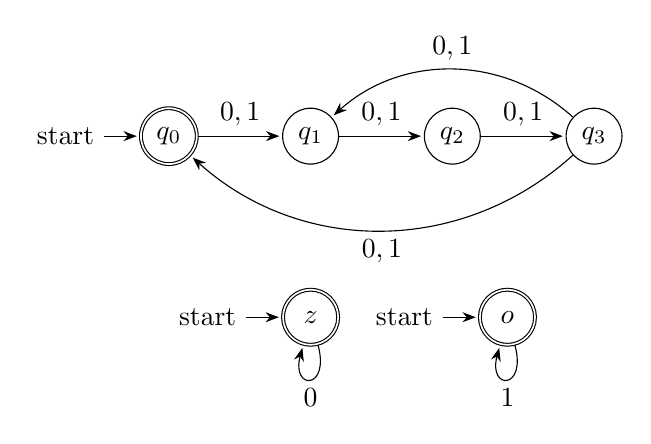
\begin{tikzpicture}[>=Stealth,shorten >=1pt,node distance=18mm,on grid,auto,
 every state/.style={minimum size=7mm},every edge/.style={draw,->}]
\node[state,initial,accepting] (q0) {$q_0$};
\node[state,right=of q0] (q1) {$q_1$};
\node[state,right=of q1] (q2) {$q_2$};
\node[state,right=of q2] (q3) {$q_3$};
\path (q0) edge node {$0,1$} (q1)
(q1) edge node {$0,1$} (q2)
(q2) edge node {$0,1$} (q3)
(q3) edge[bend left=42] node[below] {$0,1$} (q0)
(q3) edge[bend right=42] node[above] {$0,1$} (q1);
\node[state,initial,accepting,below=23mm of q1] (z) {$z$};
\node[state,initial,accepting,right=25mm of z] (o) {$o$};
\path (z) edge[loop below] node {$0$} (z)
(o) edge[loop below] node {$1$} (o);
\end{tikzpicture}
\end{center}

At length nine the only seeds are $0^9$ and $1^9$. The alternating word
$010101010$ has rank nine, forcing four parallel generations or eight
frozen-source generations. Every word of length at least ten is already a
seed. The complete length-nine counts are:
\begin{center}
\begin{tabular}{lrrrrrrrrr}
\toprule
Generation $k$ &0&1&2&3&4&5&6&7&8\\
\midrule
Parallel &2&18&186&510&512&512&512&512&512\\
Frozen-source &2&18&74&186&326&438&494&510&512\\
\bottomrule
\end{tabular}
\end{center}
The gap between $510$ and $512$ in the penultimate applicable generation
consists of the two fully alternating words.

\section{The inherited upper bound and its consequences}\label{ccc:qr:sec:upper}

Part~II of the pinned report proves that an $s$-state NFA with finite maximal
rank satisfies
\begin{equation}\label{ccc:qr:eq:upper}
R(L)\le B_s=(2s+5)^2.
\end{equation}
The source uses exact-length forward and backward reachability sets and
obtains a common eventual-periodicity threshold
\[
T_s=2(s+2)^2+2(s+2).
\]
Its periodic-interior criterion gives $R(L)\le2T_s+1=B_s$. The quadratic
unary threshold comes from To's corrected arithmetic-progression theorem
\cite[Section~3]{To}, after adding a source and a sink to normalize the unary
NFA. The source's relevant statements are its main theorem in Part~II, the
lemma headed \emph{A common quadratic transient}, the theorem headed
\emph{Interior universality criterion}, and the corollary headed
\emph{Uniform finite horizon}. This note imports that upper-bound result
rather than presenting its proof as a new contribution.

\wsevone\ These are Theorem~\ref{ccc:ps:thm:main},
Lemma~\ref{ccc:ps:lem:quadratic-period}, Theorem~\ref{ccc:ps:thm:criterion}
and Corollary~\ref{ccc:ps:cor:cutoff}; the constants are those of
\eqref{ccc:ps:eq:universal-constants}, where Part~II's $m=s+2$ is not
Part~IV's gate size.

For fixed $s$ there are only finitely many labelled NFAs up to the stated
state bound and convention. Hence the maximum defining $F(s)$ exists. Let
$D_\parallel(s)$ and $D_{\rm frozen}(s)$ be the largest finite stabilization
indices under the same convention. Proposition~\ref{ccc:qr:prop:clocks} gives
\[
D_\parallel(s)=\clog{F(s)},\qquad D_{\rm frozen}(s)=F(s)-1.
\]
Therefore Theorem~\ref{ccc:qr:thm:main} sharpens the quantitative description
to
\[
D_\parallel(s)=2\log_2 s+O(1),
\qquad
D_{\rm frozen}(s)=\Theta(s^2).
\]
The leading coefficient two in the logarithmic formula follows from the
two-sided quadratic rank bounds, including the ceiling error of less than
one.

\wsevone\ This sharpens Part~II's comment after
Theorem~\ref{ccc:ps:thm:lower-family}, which gave the order $\Theta(\log s)$
for $D_\parallel(s)$.

\paragraph{One initial state.}
If the NFA convention requires a single initial state, add a fresh accepting
source $u$ to the constructed automaton. For $a\in\Sigma$, define its
$a$-successors to be the union of the $a$-successors of the three former
initial states; make only $u$ initial and leave all old transitions and final
states unchanged. Every nonempty word is accepted exactly when it was before,
and accepting $u$ preserves the empty word. This $\eps$-free conversion adds
one state. Thus the one-initial-state version satisfies
\[
(s-4)^2\le F_{\rm one}(s)\le(2s+5)^2\qquad(s\ge5),
\]
and also has quadratic order.

\section{Attribution and remaining questions}\label{ccc:qr:sec:scope}

This result resolves an explicit asymptotic question in the inspected
repository. It does not identify an exact extremal formula. In particular,
the gap between leading constants one and four remains: the result gives
$\liminf F(s)/s^2\ge1$ and $\limsup F(s)/s^2\le4$, without proving either a
limit or a sharp constant.
\waddsevthree{Part~V proves $\limsup F(s)/s^2\le2$
(Corollary~\ref{ccc:rs:cor:upper}).}

The equal-length fragment framework and its crossover interpretation are not
claimed as new. They are developed in the ProveIt report. Closely related
represented-interval and one-point-crossover closure machinery appears
earlier in Manzoni, Vanneschi, and Mauri \cite[Definition~5.2, Theorem~5.3,
and Section~5.1]{Manzoni}; that paper treats finite populations and
logarithmic generation growth. The two-cycle graph is classical
\cite{Wielandt,Neufeld}. The specific contribution here is the
automaton-state lower-bound construction: its two monochromatic components
turn the gate's last absent length into exact maximal fragment rank. No
exhaustive priority search has been completed.

Several concrete questions remain.
\wsevone\ The manuscript lists them as an unnumbered enumeration; they are
printed as numbered questions, in the same order and words; their bracketed
titles were added.

\begin{question}[Leading constant]\label{ccc:qr:q:constant}
What is the best leading constant, or the exact function $F(s)$?
\end{question}
\waddsevthree{Part~V narrows the leading constant to $[1,2]$:
$(s-3)^2\le F(s)\le2(s-1)^2+3$ for $s\ge4$
(Corollary~\ref{ccc:rs:cor:upper}).}

\begin{question}[Order for DFAs]\label{ccc:qr:q:dfa}
What is the optimal finite-rank order for binary DFAs? The construction here
is genuinely nondeterministic: the gate has two outgoing destinations on
either letter, and the language uses a union of components. No equally small
DFA is established by this argument.
\end{question}
\wsevone\ For complete binary DFAs with at most $s$ states the bounds in this
report are $\lfloor(s-3)/2\rfloor$ (Part~II's
Theorem~\ref{ccc:ps:thm:lower-family}, whose language $L_m$ has rank $m$ and
a complete DFA with at most $2m+3$ states, $m$ being that family's index)
and $(2s+5)^2$ (every DFA is an NFA).
\waddsevthree{Part~V lowers that upper bound to $2(s-1)^2+3$, for every NFA
and so for every DFA (Corollary~\ref{ccc:rs:cor:upper}).}

\begin{question}[Tightness of the transfer principle]\label{ccc:qr:q:transfer}
How tightly can a general cofinite unary automaton's last missing length
control finite crossover rank through the transfer principle in
Remark~\ref{ccc:qr:rem:transfer}?
\end{question}

\begin{question}[Formalization]\label{ccc:qr:q:formal}
Can the lower construction and the report's upper-bound prerequisites be
formalized in a proof assistant? This note includes no Lean theorem or
machine-checked universal proof.
\end{question}
\wsevone\ This extends Part~II's Question~\ref{ccc:ps:q:formal} to Part~IV's
construction; no statement of this report is formalized.

The report's separate question about the exact decision complexity for DFA
input also remains unaffected.
\wsevone\ That is Part~II's Question~\ref{ccc:ps:q:dfa}.

\section{Reproducible finite checks}\label{ccc:qr:sec:checks}

The accompanying \texttt{check.py} uses only the Python standard library. It
constructs the transition relation, directly simulates the gate,
independently enumerates small seed slices, and compares literal fragment
partitions with the exact-length path criterion. The saved
\texttt{verification.json} records a successful run with:
\begin{itemize}
\item $147{,}677$ gate-length comparisons for $2\le m\le60$ and $0\le n\le2m^2$;
\item $8{,}184$ literal rank computations on every binary word with $2\le m\le9$ and $0\le n\le9$;
\item $8{,}222$ independent path-based rank computations, including alternating witnesses at the last missing length and the next length for $2\le m\le20$.
\end{itemize}
For the last family, the maximum tested witness rank is $361$. The path
criterion tests a fragment $w[i:j]$ by reaching its start in exactly $i$
steps, following its fixed labels, and reaching a final state in exactly
$n-j$ additional steps. It therefore enforces both alignment and total-length
matching.

These checks are finite implementation and consistency tests. They do not
establish the all-$m$ theorem, exhaust all $s$-state NFAs, prove the
inherited upper bound, determine exact $F(s)$, or verify global novelty. The
mathematical proof is in
Sections~\ref{ccc:qr:sec:gate}--\ref{ccc:qr:sec:construction}. Run
\texttt{python3 check.py} with assertions enabled; do not use Python's
\texttt{-O} option. The source file compiles with \texttt{pdflatex}; two
passes resolve internal references.

\wsevone\ \emph{Shipped layout.} The paragraphs above describe the delivered
package. In this report its files are shipped, byte-identical, as follows;
the manuscript and its PDF are printed or replaced by this report, the
delivery README by the report's README, and the checksum list
\texttt{SHA256SUMS} was verified and retired.
\begin{center}\footnotesize
\begin{tabular}{@{}P{.62\textwidth}P{.32\textwidth}@{}}
\toprule
\textbf{Shipped path} & \textbf{Delivered as}\\
\midrule
\nolinkurl{code/04-quadratic-finite-rank-check.py} & \texttt{check.py}\\
\nolinkurl{data/04-quadratic-finite-rank-verification.json} & \texttt{verification.json}\\
\nolinkurl{code/04-quadratic-finite-rank-build.sh} & \texttt{build.sh}\\
\bottomrule
\end{tabular}
\end{center}
The checker prints its record to standard output and writes no file, so it
may be run from anywhere, provided its output is not redirected onto the
shipped record:
\begin{lstlisting}
py code/04-quadratic-finite-rank-check.py > <scratch>/verification-new.json
\end{lstlisting}
(\texttt{python3} elsewhere; never with \texttt{-O}). When this Part was
written the rerun, with Python 3.14.4, took about three seconds and printed
exactly the bytes of the shipped record; a shell that writes CRLF line
endings on Windows makes the comparison hold only after normalizing them. The
build script changes to its own directory and runs \texttt{pdflatex} twice on
\texttt{quadratic-finite-rank.tex}, the delivered standalone manuscript,
which is printed here as Part~IV and is not shipped; it must not be run in
\texttt{code/}. The ``source file'' of the last paragraph above is that
manuscript; this report is built as its README describes.

%% =====================================================================
%% [write] Batch-73 addition 05: manuscript 33 of batch 73 (cluster C1),
%% "Rational Rank Slopes for Constrained Crossover". Every label of this
%% Part carries the prefix ccc:rs: (rank slopes).
%% =====================================================================
\clearpage
\phantomsection\part*{Part V.\quad Rational rank slopes for constrained crossover}
\addcontentsline{toc}{part}{Part V.\texorpdfstring{\quad}{ } Rational rank slopes for constrained crossover}

\noindent\emph{\wsevthree\ Part~V was added on 1 October 2026 in batch~73 of
ProveIt's incoming-report intake, from one manuscript written against
Parts~I--III as printed above; it knew Part~IV only as a separate
manuscript. It answers Part~II's Question~\ref{ccc:ps:q:slope} in all three
of its parts: on every live residue $r$ the largest rank $M_L(n)$ of a
length-$n$ hull word is $\sigma_rn+O(1)$, with a rational, effectively
computable slope $\sigma_r$ and without refining the period. It also proves
that longest-prefix greedy factorization into aligned fragments is optimal,
which turns the rank of one word into a linear pass, and lowers Part~II's
finite-rank bound $(2s+5)^2$ to $2(s-1)^2+3$, so that
$(s-3)^2\le F(s)\le2(s-1)^2+3$ with Part~IV's lower bound.
Section~\ref{ccc:rs:sec:provenance} records the provenance and fixes the
notation of the addition.}

\section{\texorpdfstring{\wsevthree\ }{}Provenance and notation of Part~V}
\label{ccc:rs:sec:provenance}

\subsection{One manuscript, one addition}\label{ccc:rs:sec:source}

Part~V is batch-73 manuscript~33, \emph{Rational Rank Slopes for Constrained
Crossover}, dated 1 October 2026 (11 US-letter pages as delivered). It is an
AI-assisted research note: its title page and PDF metadata read ``Research
note prepared with OpenAI for Vladimir Reshetnikov'', quoted here and in the
report's README only. It arrived as the archive
\texttt{rational-rank-slopes-package.zip} (inner directory
\texttt{rational-rank-slopes}) in ProveIt commit \texttt{f8c3a392a} and was
placed in commit \texttt{5e4f1263c}. It was written against ProveIt commit
\texttt{1bd730779} (in full
\nolinkurl{1bd730779e8bc44c8976dcd9f38cad86a0d21c26}), the pin of Part~IV's
manuscript as well; at the pin this report's \texttt{article.tex} had the
Git blob \texttt{ff492c83}, which holds Parts~I--III as printed above, so
``the pinned report'' and its ``Part~II'' in the manuscript are this report
and its Part~II. The manuscript cites its pin through a link to lines
3109--3120 of that \texttt{article.tex}, which are exactly
Question~\ref{ccc:ps:q:slope} and the comment after it. It cites the
manuscript of Part~IV, \emph{Quadratic Finite Rank for Constrained Crossover},
as a companion note; that note is Part~IV here.

Its two checkers, their recorded outputs and its build script are shipped
beside the files of Parts~I--IV with the prefix
\nolinkurl{05-rational-slopes-}; its manuscript, delivery README and PDF are
not shipped and survive in the arrival commit, and its checksum list
\texttt{SHA256SUMS} (8 files, all verified at placement) was retired by the
repository's policy. Section~\ref{ccc:rs:sec:verification} and the report's
README list the shipped names. The package contained no audit or provenance
notes; the delivery README's pin, attribution and non-claims are recorded in
this section.

Every result, proof, example, table, limitation and question of the
manuscript is printed here, in its order, with one exception: the proof of
Lemma~\ref{ccc:rs:lem:path}, which repeats Part~II's proof of the same
lemma, is replaced by a pointer (the definitions of
Section~\ref{ccc:rs:sec:periodic}, which restate Part~II's, are kept with a
pointer). Its title page
and abstract became this section; its Sections~1--10 are
Sections~\ref{ccc:rs:sec:setting}--\ref{ccc:rs:sec:verification}
(manuscript Section~$n$ is Section~$n+55$; its main theorem is
Theorem~\ref{ccc:rs:thm:slope}); it has no appendix. Its closing sentence of
next questions became
Questions~\ref{ccc:rs:q:complexity}--\ref{ccc:rs:q:error}. Text marked
\wsevthree{} was added when the manuscript was written into this report. No
theorem was strengthened or weakened.

\paragraph{What Part~V adds, and what it repeats.}
\begin{itemize}[leftmargin=1.4em,itemsep=1pt]
\item \emph{Answered:} Part~II's Question~\ref{ccc:ps:q:slope} (``On a bad
 residue, does $M_L(n)/n$ always have a limit, perhaps after refining the
 period? Must a resulting slope be rational, and can it be computed
 effectively?''), in all three parts, by Theorem~\ref{ccc:rs:thm:slope}: the
 limit exists on every live residue of every valid period, with no
 refinement; it is rational with denominator at most $p(2^s-1)$; it is the
 largest reachable cycle mean of an explicit finite graph, hence effective;
 and it is positive exactly on the residues with an interior obstruction.
\item \emph{Sharpened:} Part~II's residue-wise bounded/linear dichotomy
 (Corollary~\ref{ccc:ps:cor:residue}) becomes an exact rational slope;
 Part~II's finite-rank bound $(2s+5)^2$ (Theorem~\ref{ccc:ps:thm:main})
 becomes $2(s-1)^2+3$ (Corollary~\ref{ccc:rs:cor:upper}), by applying
 Schwarz's relation-power theorem to Part~II's bound $2t+1$, so that the
 leading constant of $F(s)$ lies in $[1,2]$ rather than Part~IV's $[1,4]$;
 Part~II's interval dynamic program for the rank of one word
 \eqref{ccc:ps:eq:rank-dp} is replaced by a linear pass
 (Corollary~\ref{ccc:rs:cor:algorithm}).
\item \emph{New:} optimality of longest-prefix greedy factorization for
 aligned fragments, for every seed language (Lemma~\ref{ccc:rs:lem:greedy},
 a positional form of a classical principle, credited as such); the
 subset-reset parser and its weighted graph
 (Proposition~\ref{ccc:rs:prop:reset}); the reciprocal slopes $1/k$; the two
 three-state examples showing that neither $t+1$ nor $\kappa+1$ replaces
 $2t+1$.
\item \emph{Restated:} Lemma~\ref{ccc:rs:lem:path} is Part~II's
 Lemma~\ref{ccc:ps:lem:fragment} with
 Corollary~\ref{ccc:ps:cor:coordinate-alphabet} (pointer; the repeated proof
 is not reprinted); Section~\ref{ccc:rs:sec:periodic} restates Part~II's
 periodic system; the parity language of Section~\ref{ccc:rs:sec:examples}
 is Part~II's Example~\ref{ccc:ps:ex:parity} with the parities exchanged;
 the bound $2t+1$ used in Corollary~\ref{ccc:rs:cor:upper} is Part~II's
 \eqref{ccc:ps:eq:transient-bound}.
\item \emph{Imported and credited:} Schwarz's theorem
 (Theorem~\ref{ccc:rs:thm:schwarz}); maximum cycle means and Karp's
 algorithm~\cite{KarpCycle}; greedy parsing (Crochemore--Langiu--Mignosi,
 De~Luca--Fici); represented-interval machinery (Manzoni--Vanneschi--Mauri);
 Part~IV's lower family.
\item \emph{Not affected:} the leading constant and the exact $F(s)$
 (Question~\ref{ccc:qr:q:constant}) remain open, now within $[1,2]$; Part~II's
 Question~\ref{ccc:ps:q:dfa} and Part~IV's Question~\ref{ccc:qr:q:dfa} on
 DFAs, Part~II's Questions~\ref{ccc:ps:q:length} and~\ref{ccc:ps:q:period}
 (to which Part~V's denominator bound and Question~\ref{ccc:rs:q:period} are
 related), and the questions of Parts~I and~III are untouched.
\end{itemize}

\subsection{The manuscript's summary and status}\label{ccc:rs:sec:abstract}

\emph{Abstract, as delivered (``the pinned ProveIt report'' is this report,
its Question~24.3 is Part~II's Question~\ref{ccc:ps:q:slope}, the companion
note is Part~IV, and the slope written $\lambda_r$ is printed $\sigma_r$).}
For a regular seed language $L$, let $M_L(n)$ be the maximum aligned-fragment
rank among length-$n$ words in its coordinate hull. On every live residue $r$
of any common eventual period of the forward and backward reachability sets,
we prove
\[
M_L(n)=\sigma_r n+O_L(1),\qquad n\equiv r\pmod p,
\]
where $\sigma_r\in[0,1]$ is rational and effectively computable. The slope is
the maximum reachable cycle mean of a finite deterministic subset-reset graph
with edge weights zero and one. The key point is that longest-prefix greedy
factorization exactly minimizes the number of aligned admissible fragments, so
the original maximum-over-words, minimum-over-partitions quantity becomes an
ordinary maximum path weight. All terminal subsets are permitted; no period
refinement is needed. This resolves the three parts of Question~24.3 in the
pinned ProveIt report. The note also gives a linear-pass fixed-word rank
algorithm after viable-layer preprocessing, examples with distinct residue
slopes and slope $1/k$, and reproducible finite checks. Separately, Schwarz's
classical relation-power bound sharpens the finite-rank estimate to
$R(L)\le2(s-1)^2+3$. Greedy parsing and cycle-mean methods are classical; no
literature-wide priority or proof-assistant verification is claimed.

\wsevthree\ The delivered abstract writes $O(1)$ where
Theorem~\ref{ccc:rs:thm:slope} writes $O_L(1)$; the constant depends on $L$
in both.

\emph{Status, as delivered.} The manuscript has no separate status box; its
abstract ends with the disclaimer above, and
Section~\ref{ccc:rs:sec:verification} states the scope of its finite checks.
Its delivery README adds: the finite checks do not prove the universal slope
theorem or Schwarz's classical theorem; the parser test covers hull targets
only and is not an exhaustive check of infinite-rank inputs or of the
empty-word branch; greedy parsing is credited to Crochemore, Langiu and
Mignosi (2014), with related discussion by De~Luca and Fici (2025), cycle
means are classical (Karp 1978), and the quadratic lower bound to the
companion note; and no global first-discovery claim, formal Lean
verification, tight slope-computation complexity, exact eventual affine
periodicity or sharp extremal constant is asserted. It also says that the
delivered PDF was compiled and every page visually inspected.

\subsection{Notation beside Parts~I--IV}\label{ccc:rs:sec:notation}

Part~V uses Part~II's notation throughout: the exact-length sets $P_i$,
$R_j$ \eqref{ccc:ps:eq:PR}, the viable layers $S_{n,i}$ and letters
$A_{n,i}$, a transient and period $t,p$, the stable sets $P^\infty_a$,
$R^\infty_a$, $S_{r,a}$, $C_{r,a}$, live residues, phase-admissible and
liftable words, interior obstructions, $M_L(n)$, $R(L)$ and $F(s)$. NFAs are
$\eps$-free, may have several initial states and need not be complete;
positions are zero based. One symbol was renamed when the manuscript was
written in: its slope $\lambda_r$, and the maximum cycle mean $\lambda$ of
Lemma~\ref{ccc:rs:lem:cycle}, are printed $\sigma_r$ and $\sigma$, because
Part~III's $\lambda_v$ is the velocity of a ray site, also a rational number
in $[0,1]$ (Section~\ref{ccc:cl:sec:notation}). No normalization changed.

\begin{center}\small
\begin{tabular}{@{}>{\raggedright\arraybackslash}p{.17\textwidth}>{\raggedright\arraybackslash}p{.39\textwidth}>{\raggedright\arraybackslash}p{.36\textwidth}@{}}
\toprule
\textbf{In Part~V} & \textbf{Meaning in Part~V} & \textbf{Not to be confused with}\\
\midrule
$\sigma_r$, $\sigma$ & rank slope on the live residue $r$; largest cycle mean (manuscript $\lambda_r$, $\lambda$) & Part~III's velocity $\lambda_v$ of a ray site\\[3pt]
bad, good & a live residue with, or without, an interior obstruction & the ``bad block'' of Part~I's Section~\ref{ccc:sec:amplification}\\[3pt]
$\rho(v)$ & least number of liftable pieces of a phase-admissible word $v$ & the rank $\rank_L(w)=\rho_L(w)$ of a hull word, which carries the language as a subscript; \eqref{ccc:rs:eq:sandwich} compares them\\[3pt]
$H_{r,a_0}(m)$, $W(m)$ & largest $\rho(v)$ over phase words of length $m$; largest path weight & Part~IV's set of gate lengths $H_m$\\[3pt]
$G_{r,a_0}$, $T_{a,c}(Z)$, $N$ & the reset graph, its transition, its vertex bound $p(2^s-1)$ & Part~III's graph $\Gamma_R$; the operator $T(L)$ and Part~II's constant $T_s$\\[3pt]
$L_n$, e.g.\ $L_3$, $L_4$ & the length-$n$ slice $L\cap\Sigma^n$ & Part~II's one-$1$ family $L_m$; Part~IV's $\Lgate m$\\[3pt]
$\kappa$, $p$ in Theorem~\ref{ccc:rs:thm:schwarz} & index and period of the powers of a relation $E$ & Part~II's period $p$ of $(P_i,R_i)$, which these imply\\
\bottomrule
\end{tabular}
\end{center}

The manuscript's macros for $\N$, $\eps$, $\rank$ and $\rec$ are the
report's; its macros \verb|\im| and \verb|\runs| are not used in its text and were
not carried over (the report's \verb|\runs| is Part~IV's). Its
\texttt{lmodern} and \texttt{amssymb} packages are not loaded (the report
keeps Part~I's newtx fonts).

\section{The question and the setting}\label{ccc:rs:sec:setting}

\wsevthree\ ``The pinned ProveIt report'' and ``the report'' of this Part are
this report as it stood at the pin, that is, Parts~I--III; ``Question~24.3''
is Part~II's Question~\ref{ccc:ps:q:slope}, and ``the companion note'' is the
manuscript of Part~IV. The manuscript's citations of both are replaced by
internal references.

Question~24.3 of the pinned ProveIt report asks whether the maximum finite rank per length has a limiting ratio on each bad residue, whether a limit must be rational, and whether it is effectively computable (Part~II, Question~\ref{ccc:ps:q:slope}). The report establishes a bounded-versus-linear dichotomy. It also identifies the central difficulty: rank is a minimum partition cost, while $M_L(n)$ maximizes that cost over targets. A cycle-mean argument requires a justified way to handle this order of quantifiers.

We consider an $\eps$-free NFA
\[
\mathcal A=(Q,\Sigma,(\Delta_c)_{c\in\Sigma},I,F),\qquad |Q|=s\ge1,
\]
over a finite nonempty alphabet, with an arbitrary set $I$ of initial states. Missing transitions are allowed. For $Z\subseteq Q$, $\Delta_c(Z)$ is the set of $c$-successors of states of $Z$; extend this notation to words by composition. Let $L$ be the accepted language and $L_n=L\cap\Sigma^n$.

For a nonempty target $w\in\Sigma^n$, an interval $[i,j)$ is \emph{admissible} if some $v\in L_n$ satisfies $v[i:j]=w[i:j]$. The aligned-fragment rank $\rank_L(w)$ is the least number of nonempty admissible intervals partitioning $[0,n)$, or infinity if none exists. Set $\rank_L(\eps)=1$ when $\eps\in L$ and infinity otherwise. The equal total length and the equal coordinates in the witnessing seed are part of this definition.

The coordinate hull is
\[
\rec(L)_n=\prod_{i=0}^{n-1}A_{n,i},\quad
A_{n,i}=\{c\in\Sigma:\exists v\in L_n,\ v_i=c\}\quad(n>0),
\]
with $\rec(L)_0=L_0$. Thus its nonempty words are exactly the words of finite rank. For $n>0$, define
\[
M_L(n)=\max\{\rank_L(w):w\in\rec(L)_n\},
\]
where the maximum is zero when the hull slice is empty. A nonempty slice gives $1\le M_L(n)\le n$.

The rank definition, coordinate hull, and relation between rank and crossover generation are existing background from the report.
\wsevthree\ They are Part~I's Definitions~\ref{ccc:def:rank} and~\ref{ccc:def:hull}
and Theorem~\ref{ccc:thm:generation}, in the zero-based form of Part~II's
Definition~\ref{ccc:ps:def:rank} and~\eqref{ccc:ps:eq:hull}; $M_L(n)$ is
Part~II's (Corollary~\ref{ccc:ps:cor:residue}). Earlier represented-interval machinery for one-point crossover appears in Manzoni, Vanneschi, and Mauri \cite{Manzoni}. The contribution pursued here is the explicit rational slope formula for regular seed languages.

\section{Why longest aligned fragments are optimal}\label{ccc:rs:sec:greedy}

\begin{lemma}[Greedy factorization of hereditary intervals]\label{ccc:rs:lem:greedy}
Fix a word on $[0,n)$. Suppose its family of admissible nonempty intervals contains every singleton and is closed under restriction to nonempty subintervals. Repeatedly taking the longest admissible interval beginning at the current boundary gives a partition with the fewest possible pieces.
\end{lemma}
\begin{proof}
Let $0=q_0<q_1<\cdots<q_k=n$ be any admissible partition, and let $g_j$ be the greedy boundaries, with $g_j=n$ after greedy has finished. Inductively, $g_j\ge q_j$. Suppose $g_{j-1}\ge q_{j-1}$. If $g_{j-1}\ge q_j$, the next greedy boundary is also at least $q_j$. Otherwise,
\[
[g_{j-1},q_j)\subseteq[q_{j-1},q_j)
\]
is a nonempty subinterval of an admissible interval and is therefore admissible. The longest extension from $g_{j-1}$ reaches at least $q_j$. This proves the induction. In particular $g_k=n$, so greedy uses at most $k$ pieces.
\end{proof}

Aligned seed fragments satisfy the hereditary hypothesis: restriction of a witnessing seed gives a witness on every smaller interval. Singletons are admissible precisely for targets in the hull. Therefore the lemma applies to every finite-rank target, for arbitrary seed languages, not only regular ones. It also applies to labelled paths through any specified sequence of viable state layers.

This is a positional form of the classical greedy-parsing principle. Crochemore, Langiu, and Mignosi study optimal greedy parsing under suffix-closure conditions for dynamic dictionaries \cite{CLM}. Their exact dynamic-dictionary convention has additional conditions, so Lemma~\ref{ccc:rs:lem:greedy} supplies the needed interval-hereditary argument directly. Factorial-language greedy optimality is also stated by De Luca and Fici \cite{DeLucaFici}. We do not claim greedy optimality itself as a new phenomenon.

\section{Viable layers and a fixed word algorithm}\label{ccc:rs:sec:parser}

Let $E$ be the unlabelled transition relation, the union of all $\Delta_c$. Write
\[
P_i=E^i(I),\qquad
R_j=\{q\in Q:\exists f\in F,\ (q,f)\in E^j\}.
\]
For a fixed total length $n$, define the viable states at boundary $i$ by
\[
S_{n,i}=P_i\cap R_{n-i}\qquad(0\le i\le n).
\]
These are exactly the states visited after $i$ letters in some accepting length-$n$ run.

\begin{lemma}[The aligned path criterion; Part~II, restated]\label{ccc:rs:lem:path}
For $0\le i<j\le n$, a word $x\in\Sigma^{j-i}$ is an admissible fragment on $[i,j)$ if and only if
\[
\Delta_x(P_i)\cap R_{n-j}\ne\varnothing.
\]
Equivalently, $x$ labels a path through the successive viable layers $S_{n,i},\ldots,S_{n,j}$. In particular,
\[
A_{n,i}=\{c\in\Sigma:\Delta_c(S_{n,i})\cap S_{n,i+1}\ne\varnothing\}.
\]
\end{lemma}
\noindent\wsevthree\ This is Part~II's Lemma~\ref{ccc:ps:lem:fragment} with its
Corollary~\ref{ccc:ps:cor:coordinate-alphabet}, and $P_i$, $R_j$, $S_{n,i}$,
$A_{n,i}$ are Part~II's \eqref{ccc:ps:eq:PR}, \eqref{ccc:ps:eq:viable-layer}
and~\eqref{ccc:ps:eq:coordinate-letters}. The manuscript credits it as
background and proves it again by the same argument (extend a path through
the viable layers backwards to an initial and forwards to a final state);
that proof is not reprinted.

For $w\in\Sigma^n$, $n>0$, precompute $S_{n,0},\ldots,S_{n,n}$. Start with $Z=S_{n,0}$ and a piece counter $b=1$. At position $i$ with letter $c=w_i$, compute
\[
U=\Delta_c(Z)\cap S_{n,i+1}.
\]
If $U\ne\varnothing$, replace $Z$ by $U$. If $U=\varnothing$, compute
\[
U'=\Delta_c(S_{n,i})\cap S_{n,i+1}.
\]
When $U'=\varnothing$, the singleton is unavailable and the rank is infinite. Otherwise increment $b$ and set $Z=U'$. At the end, return $b$.

The subset $Z$ records all possible ending states of the current greedy fragment. Failed extension closes that fragment immediately before the current letter; the letter is then consumed as the first letter of the next fragment. Because admissibility is hereditary, failure cannot be repaired by extending farther. The parser therefore realizes Lemma~\ref{ccc:rs:lem:greedy}, and its answer is the exact rank. This is a left-to-right parser with a one-letter lookahead at a boundary, after the length-dependent layers have been computed.
\wsevthree\ It replaces, for this purpose, the interval dynamic
program~\eqref{ccc:ps:eq:rank-dp} of Part~II, which tests a quadratic number of
intervals; the comparison is the write's, not the manuscript's.

\begin{corollary}[Fixed word rank complexity]\label{ccc:rs:cor:algorithm}
For an $s$-state NFA represented by Boolean transition matrices and a word of length $n>0$, exact rank is computable in
\[
O\bigl((|\Sigma|+n)s^2\bigr)
\]
time and $O(ns+s^2)$ auxiliary Boolean storage, excluding the input transition representation. If $E$ is already available, the time is $O(ns^2)$ and the auxiliary storage is $O(ns)$. For $n=0$, rank is one exactly when $I\cap F\ne\varnothing$, and infinity otherwise.
\end{corollary}
\begin{proof}
Forming $E$ costs $O(|\Sigma|s^2)$. The forward and backward recurrences and their intersections cost $O(ns^2)$. Each letter requires at most two subset images under a transition matrix, each costing $O(s^2)$. Store $O(n)$ subsets of $Q$ and, when needed, the $s\times s$ union matrix $E$. The empty-word test follows directly from $\eps$-freeness.
\end{proof}

\section{The periodic interior}\label{ccc:rs:sec:periodic}

\wsevthree\ This section restates Part~II's Section~\ref{ccc:ps:sec:dichotomy}:
\eqref{ccc:rs:eq:period} is~\eqref{ccc:ps:eq:periodicity},
\eqref{ccc:rs:eq:stable-states} and~\eqref{ccc:rs:eq:stable-alphabet} are
\eqref{ccc:ps:eq:stable-states} and~\eqref{ccc:ps:eq:stable-letters}, the
nonemptiness and agreement statement is Lemma~\ref{ccc:ps:lem:agreement}
(its two-sentence justification below repeats that proof), and
phase-admissible, liftable and interior obstruction are
Definition~\ref{ccc:ps:def:liftable}. Only the words \emph{bad} and
\emph{good} for a live residue with and without an obstruction are new;
Part~II's Question~\ref{ccc:ps:q:slope} uses ``bad residue'' in this sense.

The recurrence on pairs $(P_i,R_i)$ is deterministic and has at most $4^s$ possible values. Thus one can compute $t\ge0$ and $p\ge1$ such that
\begin{equation}\label{ccc:rs:eq:period}
P_{i+p}=P_i,\qquad R_{i+p}=R_i\qquad(i\ge t).
\end{equation}
No minimal period or sharp transient is required for the slope theorem. All phase subscripts below are interpreted modulo $p$. Set
\[
P^\infty_a=P_i\ (i\ge t,\ i\equiv a\pmod p),\qquad
R^\infty_a=R_i\ (i\ge t,\ i\equiv a\pmod p).
\]
A total-length residue $r$ is \emph{live} if $P^\infty_r\cap F\ne\varnothing$. Equivalently, every sufficiently large length in this residue has a nonempty seed slice. A nonlive residue eventually has $M_L(n)=0$.

Fix a live residue $r$ and define its stable viable states and coordinate alphabets by
\begin{align}
S_{r,a}&=P^\infty_a\cap R^\infty_{r-a},\label{ccc:rs:eq:stable-states}\\
C_{r,a}&=\{c\in\Sigma:\Delta_c(S_{r,a})\cap S_{r,a+1}\ne\varnothing\}.
\label{ccc:rs:eq:stable-alphabet}
\end{align}
All these sets are nonempty. Indeed, choose an arbitrarily long accepted length in residue $r$ and a sufficiently interior boundary in phase $a$. An accepting run supplies a state there and a letter at the next position. Moreover, for $n\equiv r\pmod p$,
\[
S_{n,i}=S_{r,i\bmod p}\quad(t\le i\le n-t),
\]
and $A_{n,i}=C_{r,i\bmod p}$ whenever both endpoints of that letter lie in this interior.

A word $v=v_0\cdots v_{m-1}$ is \emph{phase-admissible} from phase $a$ if $v_j\in C_{r,a+j}$ for every $j$. It is \emph{liftable} if it labels a path through
\[
S_{r,a},S_{r,a+1},\ldots,S_{r,a+m},
\]
starting at any state of the first layer. A phase-admissible word that is not liftable is an \emph{interior obstruction}. A live residue is \emph{bad} if such an obstruction exists at some phase, and \emph{good} otherwise. These are the periodic-interior notions used in the source report.

\section{The finite weighted reset graph}\label{ccc:rs:sec:graph}

Fix $r$ and a starting phase $a_0$. For $\varnothing\ne Z\subseteq S_{r,a}$ and $c\in C_{r,a}$, put
\[
T_{a,c}(Z)=\Delta_c(Z)\cap S_{r,a+1}.
\]
Build a letter-labelled weighted graph whose vertices are pairs $(a,Z)$ with $\varnothing\ne Z\subseteq S_{r,a}$. Its initial vertex is $(a_0,S_{r,a_0})$. For each permitted letter $c\in C_{r,a}$, the unique outgoing edge with that letter is
\begin{equation}\label{ccc:rs:eq:reset}
(a,Z)\longrightarrow
\begin{cases}
(a+1,T_{a,c}(Z)),&T_{a,c}(Z)\ne\varnothing,\quad\text{weight }0,\\
(a+1,T_{a,c}(S_{r,a})),&T_{a,c}(Z)=\varnothing,\quad\text{weight }1.
\end{cases}
\end{equation}
The reset target in the second line is nonempty by the definition of $C_{r,a}$. Retain only vertices reachable from the initial vertex and call the resulting graph $G_{r,a_0}$. There are at most
\[
N=p(2^s-1)
\]
vertices, and every retained vertex has an outgoing edge. All retained vertices are allowed as terminal vertices.

For a nonempty phase-admissible word $v$, let $\rho(v)$ be the minimum number of consecutive liftable pieces in a partition of $v$. Liftable intervals are hereditary and all singletons are liftable. Thus the greedy lemma applies.

\begin{proposition}[Rank equals one plus reset count]\label{ccc:rs:prop:reset}
Every phase-admissible word $v$ from $a_0$ labels a unique path from the initial vertex of $G_{r,a_0}$, and every such graph path is labelled by a phase-admissible word. If $|v|>0$, then
\[
\rho(v)=1+\text{the weight of its path}.
\]
Consequently, if $H_{r,a_0}(m)=\max_{|v|=m}\rho(v)$ and $W(m)$ is the maximum weight of a length-$m$ path from the initial vertex, then
\begin{equation}\label{ccc:rs:eq:H-W}
H_{r,a_0}(m)=1+W(m)\qquad(m\ge1).
\end{equation}
\end{proposition}
\begin{proof}
The transition rule is deterministic for each permitted letter and permits every phase-admissible letter sequence. Its current subset is precisely the possible endpoints of the current greedy piece. A zero-weight edge extends that piece. A weight-one edge records failure of extension, closes the previous piece, and starts the next piece with the current letter from the entire current viable layer. The first letter never causes a reset because the starting subset is that entire layer. Therefore the number of pieces is one plus the reset count, and greedy optimality makes this the minimum partition cost. Maximizing the equality over words proves \eqref{ccc:rs:eq:H-W}.
\end{proof}

This identity resolves the order-of-quantifiers issue in the source question. The minimum partition cost is computed deterministically for each target before any maximization occurs. No unjustified interchange of a maximum and a minimum is used.

\section{Cycle means with unrestricted endpoints}\label{ccc:rs:sec:cycle}

\begin{lemma}[Maximum path weight growth]\label{ccc:rs:lem:cycle}
Let $G$ be a finite directed graph with zero-one edge weights, a fixed initial vertex, and no reachable sinks. Let $W(m)$ be the maximum weight of a length-$m$ path from that vertex, with unrestricted endpoint. If $\sigma$ is the maximum mean weight of a reachable directed cycle, then
\[
W(m)=\sigma m+O(1).
\]
The maximum can be taken over simple cycles. In particular, $\sigma\in[0,1]$ is rational and effectively computable, and its reduced denominator is at most the number of reachable vertices.
\end{lemma}
\begin{proof}
Let $N$ be the number of reachable vertices. At least one reachable cycle exists, because an infinite walk can be continued without reaching a sink. Delete cycles successively from any length-$m$ path. The remaining simple path has at most $N-1$ edges. Each deleted cycle has weight at most its length times $\sigma$, and the remaining path has weight at most $N-1$. Hence
\[
W(m)\le\sigma m+N-1.
\]
For the reverse bound, choose a path of length $h$ to a cycle of length $\ell$ and mean $\sigma$. For $m\ge h$, follow that path, take $\lfloor(m-h)/\ell\rfloor$ full turns around the cycle, and take the necessary prefix of the next turn. Nonnegative edge weights give
\[
W(m)\ge\sigma(m-h-\ell+1).
\]
The finitely many smaller $m$ can be absorbed into the constant. The final partial turn is allowed because endpoints are unrestricted; there is no divisibility condition on $m$.

Every closed walk decomposes into simple cycles, and its mean is a length-weighted average of their means. Thus a maximum-mean simple cycle exists. Its mean is an integer divided by its length, at most $N$, proving rationality and the denominator bound. Finite enumeration of simple cycles proves effectivity; classical cycle-mean algorithms, such as Karp's method with signs reversed, are more efficient on an explicitly given graph \cite{KarpCycle}.
\end{proof}

The unrestricted endpoint condition is essential to this short proof. Imposing a final state could exclude some lengths and force separate congruence classes. The rank parser imposes no such condition: every subset reached after the last letter is a valid endpoint.

\section{Exact rational slopes on the original residues}\label{ccc:rs:sec:theorem}

\begin{theorem}[Residue-wise rank slope]\label{ccc:rs:thm:slope}
Let $L$ be accepted by an $s$-state $\eps$-free NFA and let $t,p$ satisfy \eqref{ccc:rs:eq:period}. For every live total-length residue $r$ there is an effectively computable rational number $\sigma_r\in[0,1]$ such that
\begin{equation}\label{ccc:rs:eq:main}
M_L(n)=\sigma_r n+O_L(1)
\qquad(n\to\infty,\ n\equiv r\pmod p).
\end{equation}
One may take $\sigma_r$ to be the maximum reachable cycle mean of $G_{r,t\bmod p}$. Its reduced denominator is at most $p(2^s-1)$. The slope is positive precisely on the bad residues, and zero on the good residues. No refinement of $p$ is needed.
\end{theorem}
\begin{proof}
Fix a sufficiently large $n>2t$ with $n\equiv r\pmod p$, and put $m=n-2t$ and $a_0=t\bmod p$. The interval $[t,n-t)$ has the stable viable-layer system beginning at phase $a_0$.

Restrict an optimal partition of a full hull word $w$ to this central interval, discard empty intersections, and apply Lemma~\ref{ccc:rs:lem:path}. The resulting pieces are liftable. Conversely, a liftable partition of the central word is a partition into admissible aligned seed fragments and can be extended by at most $2t$ singleton pieces. Therefore
\[
\rho(w[t:n-t])\le\rank_L(w)\le\rho(w[t:n-t])+2t.
\]
Every phase-admissible word of length $m$ extends to a full hull word: independently select any available letter at each boundary coordinate. These alphabets are nonempty because the seed slice is nonempty. Maximizing now gives
\begin{equation}\label{ccc:rs:eq:sandwich}
H_{r,a_0}(m)\le M_L(n)\le H_{r,a_0}(m)+2t.
\end{equation}
Proposition~\ref{ccc:rs:prop:reset} and Lemma~\ref{ccc:rs:lem:cycle} imply
$H_{r,a_0}(m)=\sigma_r m+O(1)$. Since $m=n-2t$, this proves \eqref{ccc:rs:eq:main}, rationality, the denominator bound, and effectivity.

If the residue is good, every phase-admissible word from $a_0$ is liftable, so no reset occurs and $W(m)=0$ for every $m$. Hence $\sigma_r=0$.

If the residue is bad, choose an obstruction $v$ beginning at a phase $a$. Append phase-admissible letters until it forms a block $B$ of length divisible by $p$. From any nonempty subset of $S_{r,a}$, processing the initial $v$ without a reset would give a lift of $v$ from that subset, hence from $S_{r,a}$, which is impossible. Thus each copy of $B$ forces at least one reset. From the initial vertex, a phase-admissible prefix reaches phase $a$. Repeating $B$ after this prefix gives paths with at least one reset per $|B|$ letters, so the already proved growth formula implies $\sigma_r\ge1/|B|>0$.
\end{proof}

For fixed $L,t,p$, the bounded constants may initially depend on $r$; because there are finitely many residues, one can take their maximum. Likewise, different valid transient choices produce the same slope, since \eqref{ccc:rs:eq:main} identifies it as the limit of the same ratio $M_L(n)/n$ along the residue.

\paragraph{An effective procedure.}
Compute a repeated pair in the finite process $(P_i,R_i)$, extract $t,p$, compute the stable layers and alphabets for each live $r$, explore the reachable reset graph, and compute its maximum cycle mean. This is a terminating finite procedure. It is not a claim of a tight input-complexity bound: both the period and the subset graph can be large.

\section{Examples and interpretation}\label{ccc:rs:sec:examples}

\subsection{Every reciprocal integer occurs}
Fix $k\ge2$ and let $L$ be the binary language avoiding the factor $1^{k+1}$. It is regular and its hull is universal: any prescribed singleton can be surrounded by zeroes. More generally, every block of length at most $k$ is an admissible aligned fragment at every position where it fits, since zero padding creates a seed of the required total length. Thus
\[
M_L(n)\le\left\lceil\frac nk\right\rceil.
\]
For the target $1^n$, no admissible fragment has length exceeding $k$, and partitioning into blocks of length at most $k$ attains the bound. Consequently,
\[
M_L(n)=\left\lceil\frac nk\right\rceil\quad(n\ge1),
\qquad \sigma=\frac1k.
\]
For $k=3$, a longest-prefix parser groups $1^{10}$ as $111\mid111\mid111\mid1$, giving rank four. This supplies genuinely nonintegral slopes and shows that slope denominators are unbounded over all finite automata.

\subsection{Different residues can have different slopes}
Let
\[
L=\{w\in\{0,1\}^*:|w|\text{ is odd}\}\cup0^*\cup1^*.
\]
Its hull is universal. Odd slices are already full, so $M_L(n)=1$ for odd $n$. At a positive even length, the only seeds are $0^n$ and $1^n$, so admissible fragments are exactly constant intervals. An alternating target needs $n$ fragments. Hence
\[
M_L(n)=
\begin{cases}
1,&n\text{ odd},\\
n,&n>0\text{ even},
\end{cases}
\]
and the two slopes for the natural period two are zero and one. Thus a single global limit need not exist; the residue-wise formulation is necessary.

\wsevthree\ This is Part~II's Example~\ref{ccc:ps:ex:parity} with the two
parities exchanged (there the even slices are full and the odd ones have
linear rank); the manuscript does not cite it. It is printed because it reads
the example as a statement about slopes.

\subsection{What the bounded error does and does not say}
The theorem strengthens a mere two-sided linear estimate to an exact rational leading coefficient. It does not, by itself, prove eventual equality to an affine function, exact periodicity of the bounded error, or a smallest possible error bound. In the reciprocal example, the ceiling already produces a bounded periodic fluctuation. The theorem needs no refinement of the original period to make the ratio converge.


\section{A sharper finite rank bound}\label{ccc:rs:sec:upper}

The same periodic-interior framework gives an improved quantitative bound for the finite-rank case. Define
\[
R(L)=\sup\bigl(\{1\}\cup\{\rank_L(w):w\in\rec(L)\}\bigr).
\]
The pinned report proves $R(L)\le(2s+5)^2$ when $R(L)<\infty$. Its boundary argument actually gives $2t+1$ for any valid common transient $t$.
\wsevthree\ These are Part~II's Theorem~\ref{ccc:ps:thm:main}(2) and the
bound~\eqref{ccc:ps:eq:transient-bound} of Theorem~\ref{ccc:ps:thm:criterion},
which Part~II states for any $t,p$ satisfying~\eqref{ccc:ps:eq:periodicity};
$R(L)$ is Part~II's (Corollary~\ref{ccc:ps:cor:bounded}). Applying a stronger classical relation-power theorem directly on the original state set improves the leading constant from four to two.

\begin{theorem}[Schwarz's relation-power bound, imported]\label{ccc:rs:thm:schwarz}
For every binary relation $E$ on an $s$-element set, there exist integers $\kappa,p\ge1$ such that
\[
\kappa\le(s-1)^2+1,\qquad E^{i+p}=E^i\quad(i\ge\kappa).
\]
No irreducibility assumption is required.
\end{theorem}

This is Theorem~4.3 on printed page~653 of Schwarz \cite{Schwarz}. The index is defined on printed page~634 as the least positive exponent whose relation power repeats at a later exponent; multiplying a repeated equality by further powers gives periodicity from that exponent inclusively. The theorem applies to all relations, including reducible ones. The primitive-graph exponent bound alone would not justify this application.

\begin{corollary}[Leading constant two]\label{ccc:rs:cor:upper}
For every $s$-state $\eps$-free NFA over a finite alphabet,
\[
R(L)<\infty\quad\Longrightarrow\quad R(L)\le2(s-1)^2+3.
\]
For the binary extremal function $F(s)$ under the multiple-initial-state convention, the quadratic lower family from the companion note (Part~IV, Theorem~\ref{ccc:qr:thm:main}) yields
\[
(s-3)^2\le F(s)\le2(s-1)^2+3\qquad(s\ge4).
\]
Thus the unresolved leading-constant interval narrows from $[1,4]$ to $[1,2]$.
\end{corollary}
\begin{proof}
Apply Theorem~\ref{ccc:rs:thm:schwarz} to the unlabelled relation $E$ on the original $s$ states. With $t=(s-1)^2+1$, its power identities imply both $P_{i+p}=P_i$ and $R_{i+p}=R_i$ for $i\ge t$. No source, sink, or initial-state normalization is needed.

If $R(L)<\infty$, Theorem~\ref{ccc:rs:thm:slope} shows that no live residue can be bad. For a nonempty hull word of length $n\le2t$, singleton fragments give rank at most $2t$. For $n>2t$, the central interval $[t,n-t)$ is phase-admissible in a good residue, hence liftable and, by Lemma~\ref{ccc:rs:lem:path}, one admissible seed fragment. Its two boundaries contribute at most $2t$ singleton pieces. The empty-word convention and the adjoined value one cause no exception. Therefore $R(L)\le2t+1=2(s-1)^2+3$.

The companion note (Part~IV, Theorem~\ref{ccc:qr:thm:main}) constructs an $s$-state binary NFA with exact finite rank $(s-3)^2$: an $(s-2)$-state two-cycle length gate plus two monochromatic components. Combining its lower bound with the present estimate proves the claim for $F(s)$.
\end{proof}

The statement about constants means
\[
1\le\liminf_{s\to\infty}\frac{F(s)}{s^2}
\le\limsup_{s\to\infty}\frac{F(s)}{s^2}\le2.
\]
Neither equality of these limits nor a sharp leading constant has been established.
\wsevthree\ This improves the bracket $[1,4]$ of Part~IV
(Section~\ref{ccc:qr:sec:scope}) to $[1,2]$, for NFAs. The bound
$2(s-1)^2+3$ is smaller than Part~II's $(2s+5)^2$ for every $s\ge1$.

\subsection{Why a simple one-boundary improvement fails}
The coefficient two in the boundary estimate cannot be removed merely by asserting $R(L)\le t+1$. Here is an explicit three-state example. Use states $0,1,2$, initial set $\{0,1\}$, final set $\{0\}$, and transitions
\begin{center}
\begin{tabular}{ccl}
\toprule
State & $0$-successors & $1$-successors\\
\midrule
$0$ & $\{0,2\}$ & $\varnothing$\\
$1$ & $\{0,1\}$ & $\{0\}$\\
$2$ & $\{0,1,2\}$ & $\{2\}$\\
\bottomrule
\end{tabular}
\end{center}
Here $P_i=R_i=Q$ for all $i\ge1$, so the minimal common pair transient is $t=1$ and the period is one. State $2$ has both loops, so all stable interior words lift and $R(L)\le3$. The exact length-three seed slice is
\[
L_3=\{000,001,010,100\}.
\]
The word $111$ lies in the hull, but neither of its length-two intervals is admissible. Hence its rank is three and $R(L)=3=2t+1>t+1$.

Even the full relation-power transient $\kappa$ cannot replace the two-boundary estimate by $\kappa+1$. For a second example, use initial set $\{2\}$, final set $\{0,2\}$, and transitions
\begin{center}
\begin{tabular}{ccl}
\toprule
State & $0$-successors & $1$-successors\\
\midrule
$0$ & $\{1\}$ & $\varnothing$\\
$1$ & $\{0,1\}$ & $\{1\}$\\
$2$ & $\{0\}$ & $\{2\}$\\
\bottomrule
\end{tabular}
\end{center}
Its relation powers satisfy $E^3=E^2\ne E$, so $\kappa=2$ and the period is one. Both reachability sets are $Q$ from exponent two onward; state $1$ has both loops, giving finite rank at most five. The exact length-four seed slice is
\[
L_4=\{0000,0010,1000,1110,1111\}.
\]
The hull word $0101$ has no admissible length-two interval, so its rank is four, greater than $\kappa+1=3$.
\wsevthree\ The manuscript claims only $4\le R(L)\le5$ for this automaton. A
literal computation made when the batch was placed (it is not shipped) finds
$R(L)=4$ exactly; nothing in the manuscript depends on the value. These examples do not disprove a state-count leading constant of one; they rule out two direct transient-only shortcuts to it.


\section{Reproducibility and remaining questions}\label{ccc:rs:sec:verification}

The accompanying \texttt{verify\_greedy.py} constructs accepted seed words literally, collects their actual aligned substrings, and computes the minimum partition count by interval dynamic programming. It compares this independent oracle with the viable-layer subset-reset parser. The recorded run covers every binary two-state NFA with nonempty initial and final sets through target length six, followed by $300$ seeded random NFAs on three to five states through target length eight. The seed is $20261001$.

The successful run contains $2{,}604$ automata, $14{,}407$ nonempty length slices, and $309{,}574$ rank comparisons. Only target words in nonempty coordinate hulls are compared, so these counts do not include a systematic test of infinite-rank inputs or the empty-word convention. The delivered checker prints a JSON receipt and uses only Python's standard library. Run it without the \texttt{-O} flag, since its assertions perform the comparisons.

The second checker, \texttt{check\_boundaries.py}, computes the relation-power and reachability-pair orbits, literally enumerates both displayed seed slices, and verifies the witnesses in Section~\ref{ccc:rs:sec:upper}. Its output is saved as \texttt{boundary-verification.json}.

These finite checks corroborate the parser and the faithful handling of alignment and total length. They do not prove the asymptotic theorem, exhaust all NFAs, or verify a formal proof assistant development. The universal claims are supported by the proofs above. The report's periodic-interior framework, classical greedy principles, and cycle-mean theory are credited background; the present note claims a resolution of the pinned repository question, with no assertion of global first discovery.

Natural next questions include the following.
\wsevthree\ The manuscript lists them in one sentence; they are printed as
numbered questions, in the same order and words; their bracketed titles were
added.

\begin{question}[Complexity of the slope]\label{ccc:rs:q:complexity}
What is the exact complexity of computing $\sigma_r$ from an NFA?
\end{question}

\begin{question}[Denominators]\label{ccc:rs:q:denominator}
Are there sharper denominator bounds in terms of the input structure?
\end{question}

\begin{question}[Distinguishing period]\label{ccc:rs:q:period}
What is the smallest common period needed to distinguish slopes?
\end{question}

\begin{question}[The bounded error]\label{ccc:rs:q:error}
Is the bounded error in \eqref{ccc:rs:eq:main} eventually periodic?
\end{question}

The explicit reset representation provides a finite object for studying these refinements.
\wsevthree\ Question~\ref{ccc:rs:q:period} bears on Part~II's
Question~\ref{ccc:ps:q:period}, and the denominator bound $p(2^s-1)$ of
Theorem~\ref{ccc:rs:thm:slope} on Part~II's Question~\ref{ccc:ps:q:length};
neither of those is answered. No statement of this Part is formalized; Part~II's
Question~\ref{ccc:ps:q:formal} applies to it as well.

\wsevthree\ \emph{Shipped layout.} The paragraphs above describe the delivered
package. In this report its files are shipped, byte-identical, as follows;
the manuscript and its PDF are printed or replaced by this report, the
delivery README by the report's README, and the checksum list
\texttt{SHA256SUMS} was verified and retired.
\begin{center}\footnotesize
\begin{tabular}{@{}P{.62\textwidth}P{.32\textwidth}@{}}
\toprule
\textbf{Shipped path} & \textbf{Delivered as}\\
\midrule
\nolinkurl{code/05-rational-slopes-verify_greedy.py} & \texttt{verify\_greedy.py}\\
\nolinkurl{data/05-rational-slopes-verification.json} & \texttt{verification.json}\\
\nolinkurl{code/05-rational-slopes-check_boundaries.py} & \texttt{check\_boundaries.py}\\
\nolinkurl{data/05-rational-slopes-boundary-verification.json} & \texttt{boundary-verification.json}\\
\nolinkurl{code/05-rational-slopes-build.sh} & \texttt{build.sh}\\
\bottomrule
\end{tabular}
\end{center}
Both checkers print their record to standard output and write no file, so
they may be run from anywhere, provided the output is not redirected onto a
shipped record (the report's README gives the commands). When the batch was
placed both were rerun on a copy with Python~3.14.4: the boundary checker in
about a second and the greedy checker in about seventy seconds, each printing
the bytes of its shipped record apart from CRLF line endings. The build
script changes to its own directory and runs \texttt{pdflatex} twice on
\texttt{rational-rank-slopes.tex}, the delivered manuscript, which is printed
here as Part~V and is not shipped; it must not be run in \texttt{code/}.



% [write, batch 66] the appendices belong to Part I.
\clearpage
\phantomsection\addcontentsline{toc}{part}{Appendices to Part I}
\appendix
\section{The classical universality input}\label{ccc:app:universality}

\wadd{Appendices~\ref{ccc:app:universality}--\ref{ccc:app:provenance}
belong to Part~I and are printed after Parts~II and~III so that no letter or
number of Part~I moved.}
\waddsevone{Part~IV is printed before them too.}
\waddsevthree{So is Part~V.}

For completeness, here is the standard route to the co-r.e.-completeness used
in Section~\ref{ccc:sec:undecidable}. The foundational undecidable problem is Post
correspondence~\cite{Post}. Take two morphisms $h,g:I^*\to A^*$ and ask whether
some $x\in I^+$ satisfies $h(x)=g(x)$. The set of positive instances is
recursively enumerable, and the usual effective computation-history reduction
gives r.e.-completeness.

Use disjoint alphabets $I,A$ and a separator $\$$. Among encodings
$x\$y^{\mathrm R}$, where $x\in I^+$ and $y\in A^*$, the language
\[
 \{x\$y^{\mathrm R}:y\ne h(x)\}
\]
is context-free. A pushdown automaton pushes the successive output blocks of
$h$ while reading $x$, then compares the reversed candidate output against the
stack. It accepts a symbol mismatch, a short candidate, or a long candidate;
the regular encoding conditions can be imposed separately. The analogous
language for $g$ is also context-free. Their union, together with all malformed
encodings, is universal exactly when the correspondence instance has no
solution. This proves co-r.e.-hardness of grammar universality. Its complement
is r.e. because grammar membership is decidable and nonmembers can be searched
for by length.

To obtain a binary alphabet, map each letter of the finite encoding alphabet
to a distinct binary block of one common length $\ell$. For a language $H$
over that alphabet, set
\[
 H'=c(H)\cup\bigl(\{0,1\}^*\setminus c(A_0^*)\bigr),
\]
where $A_0$ denotes the entire encoding alphabet. The image $c(H)$ is
context-free and $c(A_0^*)$ is regular. The injective fixed-length code gives
$H'=\{0,1\}^*$ exactly when $H=A_0^*$. This is a reduction for universality;
as Section~\ref{ccc:sec:questions} emphasizes, it is \emph{not} automatically a
reduction preserving crossover.

\section{Why the positional counts are eventually affine}
\label{ccc:app:counting}

The special case of Presburger counting needed here also has a direct
one-dimensional explanation. After quantifier elimination, a predicate in
variables $(n,i)$ is a Boolean combination of linear inequalities and fixed
modular congruences. We also impose $0\leq i<n$.

Refine the residue class of $n$ modulo all congruence moduli, and refine the
residue class of $i$ similarly. On these classes, congruences have constant
truth values. Each nontrivial inequality in $i$ changes truth value at a
rational-affine threshold in $n$. The order of finitely many such thresholds
is fixed once $n$ is sufficiently large: two affine functions either agree
identically or their order changes at most once.

Thus the allowed positions eventually form a fixed finite union of intervals
between affine thresholds, possibly with selected endpoint positions, in each
fixed residue class of $i$. Counting that class inside such an interval is a
difference of floor or ceiling functions of rational-affine expressions.
Refine the period of $n$ to absorb the finitely many denominators. Each such
count then is affine on a progression. Finite union and disjoint refinement
preserve that property.

This argument explains both effectivity and the degree-one conclusion of
Lemma~\ref{ccc:lem:affinecounts}; the general counting theorem of Woods supplies a
systematic framework. Since counts are nonnegative for all sufficiently large
parameters and integer-valued, their progression increments are nonnegative
integers. That final observation is what makes the geometric factors in
Theorem~\ref{ccc:thm:rational} polynomials rather than Laurent expressions.

\section{A compact proof-dependency map}\label{ccc:app:dependencies}

\begin{center}\small
\begin{tabular}{@{}p{.37\textwidth}p{.56\textwidth}@{}}
\toprule
\textbf{Result} & \textbf{Essential inputs}\\
\midrule
Exact contraction and generation &
Definition of aligned crossover; restriction and pairing of consecutive
intervals. No grammar theorem.\\[3pt]
One-step CFG undecidability &
One-cut guard repair; classical fixed-binary CFG universality.\\[3pt]
Eventual CFG undecidability &
Exact generation; disjoint boundary intervals for forbidden blocks;
effective CFL union, concatenation, and star.\\[3pt]
Regular-input stabilization &
Exact generation; explicitly constructed distance automaton; classical
limitedness decidability.\\[3pt]
Rational weighted hull series &
Effective Parikh semilinearity; one-parameter Presburger counting;
coordinate-product enumeration.\\[3pt]
Non-CFL linear-seed example &
Explicit grammar; elementary position inequalities; CFL pumping lemma and
intersection with a regular language.\\[3pt]
Minimal finite-stage recurrence &
Exact binomial count; degree of a polynomial; reduced rational denominators.\\
\bottomrule
\end{tabular}
\end{center}

\section{\texorpdfstring{\wtag\ }{}Provenance of this report}\label{ccc:app:provenance}

\paragraph{One manuscript.} This report is built from a single manuscript,
manuscript~02 of batch~44 of ProveIt's incoming-report intake:
\emph{Aligned Fragments and Constrained Crossover}, dated 29 September 2026,
delivered as the archive \texttt{ProveIt\_Constrained\_Crossover.zip}, which
arrived in commit \texttt{ae28ea2db} and was placed in commit
\texttt{203016015}. Its pin is ProveIt commit
\texttt{9b24a3a8d545af9624f6ac455f5b548be62818b6} (Section~\ref{ccc:sec:intro}).
The manuscript contributed everything outside the text marked \wtag: every
result, proof, example, remark, question, limitation and the Lean plan, all
printed. The package's audit notes and verifier are shipped unchanged beside
this article (Section~10.2 lists the paths). Its 23-page US-letter PDF and its
README are not shipped; they survive in the arrival commit.
\wadd{this describes Part~I; Parts~II and~III come from two further
manuscripts (last paragraph of this appendix).}

\paragraph{What the write added.} Everything marked \wtag: the title-page
note; in Section~\ref{ccc:sec:intro}, where Hughes poses the question, the state
of the sibling source, and Sections~\ref{ccc:sec:sibling}
and~\ref{ccc:sec:notation}; the note after Remark~2.3; the notes on the
shipped layout and on formal status in Section~\ref{ccc:sec:verification}; the
note on Hughes's Sections~13--14 after the research questions; and this
appendix. The locations in Hughes's preprint were checked against its
arXiv~v1 PDF when the report was written.

\paragraph{Choices.} There was no merge, so no result had to be chosen over
another. Every label received the prefix \texttt{ccc:}, and every reference
was updated with it. Labels were added only on new text and on
Question~\ref{ccc:q:arithmetical} and Section~\ref{ccc:sec:lean}; no theorem,
section or equation number of the manuscript changed. The page size stays US
letter, as delivered. No symbol was renamed; the \texttt{shuffle} package was
added for the symbol $\sh$ of the sibling report.

\paragraph{\wadd{Two further manuscripts.}} This appendix describes the
report as written in batch~44, which is Part~I. On 30 September 2026 two
manuscripts of batch~66, both written against Part~I at ProveIt commit
\texttt{b8b0fa218} (where Part~I's text was the one printed here), were added
as Parts~II and~III: manuscript~01, \emph{Finite Crossover Stabilization Is
PSPACE-Complete} (archive \texttt{ProveIt\_Crossover\_Stabilization.zip}),
and manuscript~03, \emph{Decidable Regularity and Exact Stabilization of
Crossover Closures} (archive \texttt{ProveIt\_Crossover\_Classification.zip}).
Both arrived in commit \texttt{9ad899cbe} and were placed in commit
\texttt{4fee1cd07}. The report is therefore built from three manuscripts.
Sections~\ref{ccc:ps:sec:source} and~\ref{ccc:cl:sec:source} give each one's
provenance and what it contributed. The choices made were these. The two
were kept as separate Parts, not merged, because they share no main theorem;
the only overlap is a reproof of Part~I's coordinate hull, printed once
(Theorem~\ref{ccc:thm:generation}) with the two reproofs kept as marked second
and third routes (Proposition~\ref{ccc:ps:prop:rank-clock},
Lemma~\ref{ccc:cl:lem:hull}). Part~III's Lemma~\ref{ccc:cl:lem:presburger},
which restates Part~I's Lemma~\ref{ccc:lem:positions} without citing it, now
credits it, and its proof is kept as a second route. Every label of the two
manuscripts received the prefix \texttt{ccc:ps:} or \texttt{ccc:cl:}; their
appendices became sections, because the appendices belong to Part~I; ten
symbols were renamed where they clash (Sections~\ref{ccc:ps:sec:notation}
and~\ref{ccc:cl:sec:notation}); the bibliographies were merged (each
manuscript's entry for Part~I replaced by internal references, its
Hughes entry identified with Part~I's, and Part~III's Esparza et~al.\ entry
with \cite{EGKL}). Four labels were added to existing text of Part~I
(\texttt{ccc:q:regular}, \texttt{ccc:q:grammar}, \texttt{ccc:q:series},
\texttt{ccc:q:restricted} on its questions) and dated notes were added after
Corollary~\ref{ccc:cor:regularstability}, after four of its questions, in its
Sections~\ref{ccc:sec:verification}--\ref{ccc:sec:questions}, in its
conclusion, on the title page, and here; no existing label, theorem, section,
equation or question number of Part~I changed.

\paragraph{\waddsevone{A fourth manuscript.}} On 1 October 2026 batch-71
manuscript~01, \emph{Quadratic Finite Rank for Constrained Crossover}
(archive \texttt{quadratic-finite-rank-package.zip}), written against
Parts~I--III at ProveIt commit \texttt{1bd730779}, which arrived in commit
\texttt{aee32ad45} and was placed in commit \texttt{427bca743}, became
Part~IV. The report is now built from four manuscripts;
Section~\ref{ccc:qr:sec:source} gives this one's provenance and what it
contributed. The choices made were these. Part~IV answers Part~II's
Question~\ref{ccc:ps:q:rank} and imports Part~II's upper bound; it was kept
as a Part of its own, not merged into Part~II, because its construction is
new and shares no proof with Part~II. Its restatement of the rank calculus
is printed as a marked restatement with its proof as one more route
(Proposition~\ref{ccc:qr:prop:clocks}); its last-gap lemma received a
credit to Sylvester's two-generator Frobenius formula; its gate language was
renamed $\Lgate m$, because Part~II's $L_m$ is another family; its four
unnumbered questions received numbers and labels; every label received the
prefix \texttt{ccc:qr:}; its bibliography entry for the pinned report was
replaced by internal references, its To entry identified with \cite{To},
and two entries (Sylvester, Ram\'irez Alfons\'in) were added for the credit.
Dated notes were added in Part~I's
Section~\ref{ccc:sec:verification}, its conclusion and
Appendix~\ref{ccc:app:universality}, in Part~II's delivered status, after
Theorem~\ref{ccc:ps:thm:lower-family}, after
Questions~\ref{ccc:ps:q:rank} and~\ref{ccc:ps:q:formal}, in Part~II's
conclusion, and here (the title page, already full, received none); no
existing label, theorem, section, equation or
question number changed.

\paragraph{\waddsevthree{A fifth manuscript.}} On 1 October 2026 batch-73
manuscript~33, \emph{Rational Rank Slopes for Constrained Crossover}
(archive \texttt{rational-rank-slopes-package.zip}), written against
Parts~I--III at ProveIt commit \texttt{1bd730779}, which arrived in commit
\texttt{f8c3a392a} and was placed in commit \texttt{5e4f1263c}, became
Part~V. The report is now built from five manuscripts;
Section~\ref{ccc:rs:sec:source} gives this one's provenance and what it
contributed. The choices made were these. Part~V answers Part~II's
Question~\ref{ccc:ps:q:slope} and was kept as a Part of its own, because its
theorem and its proof (greedy optimality, the subset-reset graph, cycle
means) are new; its restatement of Part~II's aligned fragment criterion
became a pointer without the repeated proof, its periodic definitions and
its parity example are kept with pointers to Part~II; its slope $\lambda_r$
was renamed $\sigma_r$, because Part~III's $\lambda_v$ is another rational
quantity; its sentence of next questions became four numbered questions;
every label received the prefix \texttt{ccc:rs:}; its bibliography entries
for the pinned report and for Part~IV's manuscript were replaced by internal
references, its Manzoni entry identified with \cite{Manzoni}, and its
Karp~(1978) entry printed as \cite{KarpCycle}, because \cite{Karp} is another
paper. Dated notes were added after Questions~\ref{ccc:ps:q:rank},
\ref{ccc:ps:q:slope}, \ref{ccc:qr:q:constant} and~\ref{ccc:qr:q:dfa}, after Part~II's fixed-word
algorithm and Corollary~\ref{ccc:ps:cor:residue}, in Part~II's conclusion,
in Part~I's conclusion, in Part~IV's Section~\ref{ccc:qr:sec:scope}, in
Appendix~\ref{ccc:app:universality} and here; no existing label, theorem,
section, equation or question number changed.

\begin{thebibliography}{99}
\small\raggedright\setlength{\itemsep}{1pt}\setlength{\parsep}{0pt}\setlength{\parskip}{0pt}
\bibitem{Hughes}
Charles E. Hughes.
\emph{Undecidability of Adjacent Equality for Insertion, Shuffle, and Crossover
Language Operations}.
arXiv:2608.27755v1, 27 August 2026.
Definition on printed p.~2; the constrained one-step question on printed p.~3.
\wtag\ Section~2 (definition), Section~4 (the question, pp.~3--4),
Section~14 (open directions, p.~12).
\url{https://arxiv.org/abs/2608.27755v1}.

\bibitem{Repo}
Vladimir Reshetnikov and ProveIt contributors.
\emph{ProveIt: Gaps in Bounded-Shuffle Hierarchies}, Parts~I--II.
Inspected 29 September 2026 at the revision and path specified in
Section~\ref{ccc:sec:intro}. AI-assisted research drafts.
\wtag\ The sibling report \texttt{insertion-degree-spectra} of this
collection (Section~\ref{ccc:sec:sibling}).
\url{https://github.com/VladimirReshetnikov/ProveIt}.

\bibitem{EGKL}
Javier Esparza, Pierre Ganty, Stefan Kiefer, and Michael Luttenberger.
Parikh's theorem: A simple and direct automaton construction.
\emph{Information Processing Letters} \textbf{111}(12) (2011), 614--619.
\url{https://arxiv.org/abs/1006.3825}.
\href{https://doi.org/10.1016/j.ipl.2011.03.019}{doi:10.1016/j.ipl.2011.03.019}.

\bibitem{Woods}
Kevin Woods.
Presburger arithmetic, rational generating functions, and quasi-polynomials.
\emph{Journal of Symbolic Logic} \textbf{80} (2015), 433--449.
\url{https://arxiv.org/abs/1211.0020}.
\href{https://doi.org/10.1017/jsl.2015.4}{doi:10.1017/jsl.2015.4}.

\bibitem{Kirsten}
Daniel Kirsten.
Distance desert automata and the star height problem.
\emph{RAIRO---Theoretical Informatics and Applications}
\textbf{39}(3) (2005), 455--509.
\url{https://www.numdam.org/item/ITA_2005__39_3_455_0/}.
\href{https://doi.org/10.1051/ita:2005027}{doi:10.1051/ita:2005027}.

\bibitem{KMT}
Markus Kr\"otzsch, Tom\'a\v{s} Masopust, and Micha\"el Thomazo.
Complexity of universality and related problems for partially ordered
NFAs. \emph{Information and Computation} \textbf{255}, Part 1 (2017), 177--192.
Preprint arXiv:1609.03460v2.
\url{https://arxiv.org/abs/1609.03460}.

\bibitem{Post}
Emil L. Post.
A variant of a recursively unsolvable problem.
\emph{Bulletin of the American Mathematical Society}
\textbf{52} (1946), 264--268.

% [write, batch 66] entries cited by Parts II and III. Their entries for
% Part I itself were replaced by internal references; their Hughes entries are
% \cite{Hughes} above; Part III's Esparza et al. entry is \cite{EGKL} above.
\bibitem{To}
Anthony Widjaja To.
\emph{Unary finite automata vs. arithmetic progressions}.
\emph{Information Processing Letters} 109(17) (2009), 1010--1014.
Corrected proof in Section~3 of arXiv:0812.1291v1.
\url{https://arxiv.org/abs/0812.1291}.
DOI: \nolinkurl{10.1016/j.ipl.2009.06.005}.

\bibitem{KRS}
Jui-Yi Kao, Narad Rampersad, and Jeffrey Shallit.
\emph{On NFAs Where All States are Final, Initial, or Both}.
\emph{Theoretical Computer Science} 410(47--49) (2009), 5010--5021.
Lemma~6 in arXiv:0808.2417v2, revised 3 July 2009.
\url{https://arxiv.org/abs/0808.2417}.
DOI: \nolinkurl{10.1016/j.tcs.2009.07.049}.

\bibitem{Savitch}
Walter J. Savitch.
\emph{Relationships between nondeterministic and deterministic tape
complexities}.
\emph{Journal of Computer and System Sciences} 4(2) (1970), 177--192.
DOI: \nolinkurl{10.1016/S0022-0000(70)80006-X}.

\bibitem{Parikh}
Rohit J. Parikh.
On context-free languages.
\emph{Journal of the ACM} \textbf{13}(4) (1966), 570--581.
\href{https://doi.org/10.1145/321356.321364}{doi:10.1145/321356.321364}.

\bibitem{GinsburgSpanier}
Seymour Ginsburg and Edwin H. Spanier.
Semigroups, Presburger formulas, and languages.
\emph{Pacific Journal of Mathematics} \textbf{16}(2) (1966), 285--296.
\href{https://doi.org/10.2140/pjm.1966.16.285}{doi:10.2140/pjm.1966.16.285}.

\bibitem{Barcelo}
Pablo Barcel\'o, Chih-Duo Hong, Xuan-Bach Le, Anthony W. Lin, and Reino Niskanen.
Monadic decomposability of regular relations.
In \emph{ICALP 2019}, LIPIcs \textbf{132}, article 103.
\href{https://doi.org/10.4230/LIPIcs.ICALP.2019.103}{doi:10.4230/LIPIcs.ICALP.2019.103}.

\bibitem{Hague}
Matthew Hague, Anthony W. Lin, Philipp R\"ummer, and Zhilin Wu.
Monadic decomposition in integer linear arithmetic.
In \emph{IJCAR 2020, Part I}, LNCS \textbf{12166}, 122--140.
\href{https://doi.org/10.1007/978-3-030-51074-9_8}{doi:10.1007/978-3-030-51074-9\_8}.
Extended version: \url{https://arxiv.org/abs/2004.12371}.

\bibitem{Ganardi}
Moses Ganardi and Marin Ricros.
Constructing small monadic decompositions in Presburger arithmetic.
In \emph{LICS 2026}, LIPIcs \textbf{380}, 47:1--47:22.
Published 9 July 2026.
\href{https://doi.org/10.4230/LIPIcs.LICS.2026.47}{doi:10.4230/LIPIcs.LICS.2026.47}.

\bibitem{Raz}
Danny Raz.
Length considerations in context-free languages.
\emph{Theoretical Computer Science} \textbf{183}(1) (1997), 21--32.
\href{https://doi.org/10.1016/S0304-3975(96)00308-8}{doi:10.1016/S0304-3975(96)00308-8}.

\bibitem{Karp}
Richard M. Karp.
Reducibility among combinatorial problems.
In R. E. Miller and J. W. Thatcher (eds.),
\emph{Complexity of Computer Computations}, Plenum, 1972, 85--103.
\href{https://doi.org/10.1007/978-1-4684-2001-2_9}{doi:10.1007/978-1-4684-2001-2\_9}.

\bibitem{Rosser}
J. Barkley Rosser and Lowell Schoenfeld.
Approximate formulas for some functions of prime numbers.
\emph{Illinois Journal of Mathematics} \textbf{6}(1) (1962), 64--94.
\href{https://doi.org/10.1215/ijm/1255631807}{doi:10.1215/ijm/1255631807}.

% [write, batch 71] entries cited by Part IV. Its entry for this report was
% replaced by internal references; its To entry is \cite{To} above; the
% last two entries support the write's credit after Lemma ccc:qr:lem:gap.
\bibitem{Manzoni}
Luca Manzoni, Leonardo Vanneschi, and Giancarlo Mauri.
\emph{A distance between populations for one-point crossover in genetic algorithms}.
\emph{Theoretical Computer Science} 429 (2012), 213--221.
DOI: \nolinkurl{10.1016/j.tcs.2011.12.041}.
Author-repository full text:
\url{https://run.unl.pt/server/api/core/bitstreams/1639e177-ebcc-4aa6-baf2-ab9778007dd2/content}.

\bibitem{Wielandt}
Helmut Wielandt.
\emph{Unzerlegbare, nicht negative Matrizen}.
\emph{Mathematische Zeitschrift} 52 (1950), 642--648.
DOI: \nolinkurl{10.1007/BF02230720}.

\bibitem{Neufeld}
Stewart W. Neufeld.
\emph{A diameter bound on the exponent of a primitive directed graph}.
\emph{Linear Algebra and its Applications} 245 (1996), 27--47.
DOI: \nolinkurl{10.1016/0024-3795(94)00203-7}.

\bibitem{Sylvester}
J. J. Sylvester.
\emph{Mathematical questions with their solutions}.
\emph{Educational Times} 41 (1884), 21.

\bibitem{RamirezAlfonsin}
Jorge L. Ram\'irez Alfons\'in.
\emph{The Diophantine Frobenius Problem}.
Oxford Lecture Series in Mathematics and its Applications 30,
Oxford University Press, 2005.

% [write, batch 73] entries cited by Part V. Its entries for this report and
% for Part IV's manuscript were replaced by internal references; its Manzoni
% entry is \cite{Manzoni} above; its Karp entry is KarpCycle, since Karp
% above is another paper.
\bibitem{CLM}
Maxime Crochemore, Alessio Langiu, and Filippo Mignosi.
Note on the greedy parsing optimality for dictionary-based text compression.
\emph{Theoretical Computer Science} \textbf{525} (2014), 55--59.
\href{https://doi.org/10.1016/j.tcs.2014.01.013}{doi:10.1016/j.tcs.2014.01.013}.
\href{https://arxiv.org/abs/1211.5350}{arXiv:1211.5350}.

\bibitem{DeLucaFici}
Alessandro De Luca and Gabriele Fici.
Dorst--Smeulders coding for arbitrary binary words.
\href{https://arxiv.org/abs/2509.08684v1}{arXiv:2509.08684v1} (10 September 2025).

\bibitem{KarpCycle}
Richard M. Karp.
A characterization of the minimum cycle mean in a digraph.
\emph{Discrete Mathematics} \textbf{23}(3) (1978), 309--311.
\href{https://doi.org/10.1016/0012-365X(78)90011-0}{doi:10.1016/0012-365X(78)90011-0}.

\bibitem{Schwarz}
\v{S}tefan Schwarz.
On the semigroup of binary relations on a finite set.
\emph{Czechoslovak Mathematical Journal} \textbf{20}(95) (1970), no.~4, 632--679.
Theorem~4.3, p.~653; index definition, p.~634.
\href{https://doi.org/10.21136/CMJ.1970.100989}{doi:10.21136/CMJ.1970.100989}.
\href{https://dml.cz/bitstream/handle/10338.dmlcz/100989/CzechMathJ_20-1970-4_9.pdf\#page=23}{Primary full text, theorem page}.
\end{thebibliography}
\end{document}
